\chapter{Combining Basic Covariance Functions}
\label{chapCombiningBasicCovariances}

\begin{mdframed}[hidealllines=true,backgroundcolor=lightgray!20]
\section*{Résumé}
Souvent, le type d'information initiale que nous voulons intégrer n'est pas disponible sous la forme de fonctions de covariance basiques. Heureusement, plusieurs nouveaux noyaux peuvent être créés en fusionnant les noyaux de base que nous avons vus dans le chapitre précédent. Ce chapitre est inspiré par les travaux de  \cite{bishop2006pattern, mackay2003information, durrande2001etude, durrande2013anova}.


La section \ref{secSingleDimension} décrit comment combiner les noyaux pour créer des noyaux unidimensionnels. Nous fournissons une explication intuitive de ce qui se produit lorsque nous ajoutons ou multiplions des noyaux, ces types de noyaux peuvent être utilisés pour détecter et séparer les modèles de données. La section \ref{subsubsecCh4ApplicationCP} décrit comment créer des noyaux pour des dimensions plus élevées. Ce type de noyaux peut être utilisé pour effectuer une analyse de sensibilité ou projeter les données en dimension plus faibles.


Dans ce chapitre, nous utilisons une combinaison de noyaux de base pour identifier l'apparition de non linéarités dans les systèmes physiques. Par exemple, nous identifions l'initiation de la séparation de l'écoulement pour le profil d'aile NACA 0012 et l'initiation de la plasticité pour l'alliage AL6061 en utilisant un critère statistique pour la détection automatique de la non-linéarité (section \ref{subsubsecCh4ApplicationCP}) \cite{chiplunkar:hal-01555401}. Nous construisons enfin un modèle de GP pour prédire la position du choc aérodynamique en régime transsonique (section \ref{subecInterpolationOfAerodynamicPressures}) \cite{oatao18004}.
\end{mdframed}


%\pagebreak

\section{Introduction}

What if the kind of patterns that we wish to encode are not possible by using the basic kernels described in chapter \ref{chapBasicCovarianceKernels}? What if we wish to encode several different patterns in our hypothesis space? Or what if we want to build models for data-sets with more than one input dimension? Thankfully, many new kernels can be constructed by merging a few basic kernels, this chapter answers the above questions. 

The original contribution of this chapter is applying the newly created covariance functions to create engineering design models. The set of equations below are a few simple methods to create valid covariance functions \cite{bishop2006pattern, mackay2003information, durrande2001etude, durrande2013anova}. 

\begin{align}
k(x_{1}, x_{2}) =  & k_{1}(x_{1}, x_{2}) + k_{2}(x_{1}, x_{2})  \label{eqCh5AddingCovariances} \\
k(x_{1}, x_{2}) =  & k_{1}(x_{1}, x_{2}) \times k_{2}(x_{1}, x_{2}) \label{eqCh5MultiplyingCovariances} \\
k(x_{1}, x_{2}) =  & q(x_{1})k_{1}(x_{1}, x_{2})q(x_{2}) \label{eqCh5MultiplyingWithFunction} \\
k(x_{1}, x_{2}) =  & k_{1}(h(x_{1}), h(x_{2})) \label{eqCh5ComposedCovariances} \\
k(x_{1}, x_{2}) =  & g(g(k_{1}(x_{1}, x_{2}), x_{1}), x_{2} ) \label{eqCh5LinearOperatorCovariances} \\
k(x_{1}, x_{2}) = & \int k_{1}(x_{1}, u)k_{2}(u, x_{2})du \label{eqConvolutionProcess}
\end{align}


Here, $k_{1}(x_{1}, x_{2})$ and $k_{2}(x_{1}, x_{2})$ are valid covariance function, while $q(x)$ and $h(x)$ are any continuous functions. Equation \ref{eqConvolutionProcess} defines a covariance function through convolution of two kernels, while equation \ref{eqCh5LinearOperatorCovariances} defines transformation through a linear operator $g\left ( . \right ) \in \mathcal{C}^{2}$, for more discussion on this equation refer to chapter \ref{chapAddingEquationsInGP}. 

Let us take the case of a 2-dimensional input vector\footnote{The superscript is used to denote the number of dimension and does not denote the power.} $\VEC{x}$ such that $\VEC{x} = \{x^{1}, x^{2}\}$ ($x^{1}$, $x^{2}$ are coordinates of $\VEC{x}$ in the first and second dimension respectively). Then the following covariance functions are also valid.

\begin{align}
k(\VEC{x_{1}}, \VEC{x_{2}}) = k_{1}(x_{1}^{1}, x_{2}^{1}) + k_{2}(x_{1}^{2}, x_{2}^{2}) \label{eqCh5AddingAcrossDimensionsCovariances} \\
k(\VEC{x_{1}}, \VEC{x_{2}}) = k_{1}(x_{1}^{1}, x_{2}^{1}) \times k_{2}(x_{1}^{2}, x_{2}^{2}) \label{eqCh5MultiplyingAcrossDimensionsCovariances} 
\end{align}

The current chapter is written to provide intuition on what happens when we combine covariance functions. This chapter unfolds as follows; section \ref{secSingleDimension} provides intuition on combining kernels for one-dimensional inputs, while section \ref{secMultiDimensionalKernels} details how to create covariance functions for higher-dimensions (equation \ref{eqCh5AddingAcrossDimensionsCovariances} and \ref{eqCh5MultiplyingAcrossDimensionsCovariances}) inputs. We then apply the newly constructed kernels, to first detect onset of non-linearity in experimental data, and later interpolate the shock pressures on a CRM wing in transonic regime.

\section{One dimensional inputs}\label{secSingleDimension}
Combining kernels can give rise to interesting features, in this section we provide intuition on combining kernels in one dimension. Section \ref{subsecStructureKernelsMultiplyingKernels} details effects of multiplying kernels (equation \ref{eqCh5MultiplyingCovariances}) while section \ref{subsecStructureKernelsAddingKernels} describes effects of adding kernels (equation \ref{eqCh5AddingCovariances}). Section \ref{subsubsecCh4ApplicationCP} describes the Change-Point (CP) kernel. We use the CP kernel to detect start of plasticity in elastic structures such as beams and start of flow separation on an airfoil \cite{chiplunkar:hal-01555401}. 


\subsection{Multiplying Kernels} \label{subsecStructureKernelsMultiplyingKernels}
Multiplying two covariance functions acts as an AND operator, the resulting kernel has high value only if we have high value on both the kernels. Multiplying a Linear kernel $L$ times, will result in a $L^{th}$ order polynomial regression (equation \ref{eqCh4PolynomialCovariance}). 

\begin{equation}\label{eqCh4PolynomialCovariance}
k_{Lin} = w_{0} + w_{1}x_{1}^T x_{2} \quad k_{Poly} = \prod_{i=1}^{L} \left (w_{0}^{i} + w_{1}^{i}x_{1}^T x_{2} \right)
\end{equation}

Equation \ref{eqMultiLinSECovariance} shows the prior obtained after multiplying a Linear and a SE kernel. This covariance function resembles a SE covariance function but with the amplitude hyper-parameter ($\theta_{amplitude} = \textcolor{red}{x_{1}x_{2}}$) proportional to the  distance. 

\begin{equation}\label{eqMultiLinSECovariance}
k_{Multi} = \textcolor{red}{x_{1}x_{2}} exp[- \frac{d^2}{2}]
\end{equation}

\marginnote{\textsl{Figure \ref{subFigPriorMultiLinSE}}}[1cm]
Figure \ref{subFigPriorMultiLinSE} shows random draws obtained using $k_{Multi}$ covariance,  the hyper-parameters of the linear kernel are $w_{0}=0$ and $w_{1}=1$, this means that there is no intercept and $k_{Lin}(x_{1}, x_{2}) = x_{1}x_{2}$. The hyper-parameters of the SE part are $\theta_{amplitude}=1$ and $\theta_{lengthScale}=1$, similar to figure \ref{subFigpriorDrawsSE}. Since multiplying two kernels is an AND operation, $k_{Multi}$ tends to zero at $x=0$ since $k_{Lin}$ is zero at $x=0$. 

\begin{figure}[!ht]
  \centering
    \subfigure[{Draws from a GP prior with mean zero and kernel obtained by \textbf{multiplying} a Linear kernel with SE kernel. The hyper-parameters of the linear kernel are $w_{0}=0$ and $w_{1}=1$ while the hyper-parameters of the SE part are $\theta_{amplitude}=1$ and $\theta_{lengthScale}=1$. We see that the variance at $x=0$ goes to zero, since multiplication is an AND operation}]
  {
        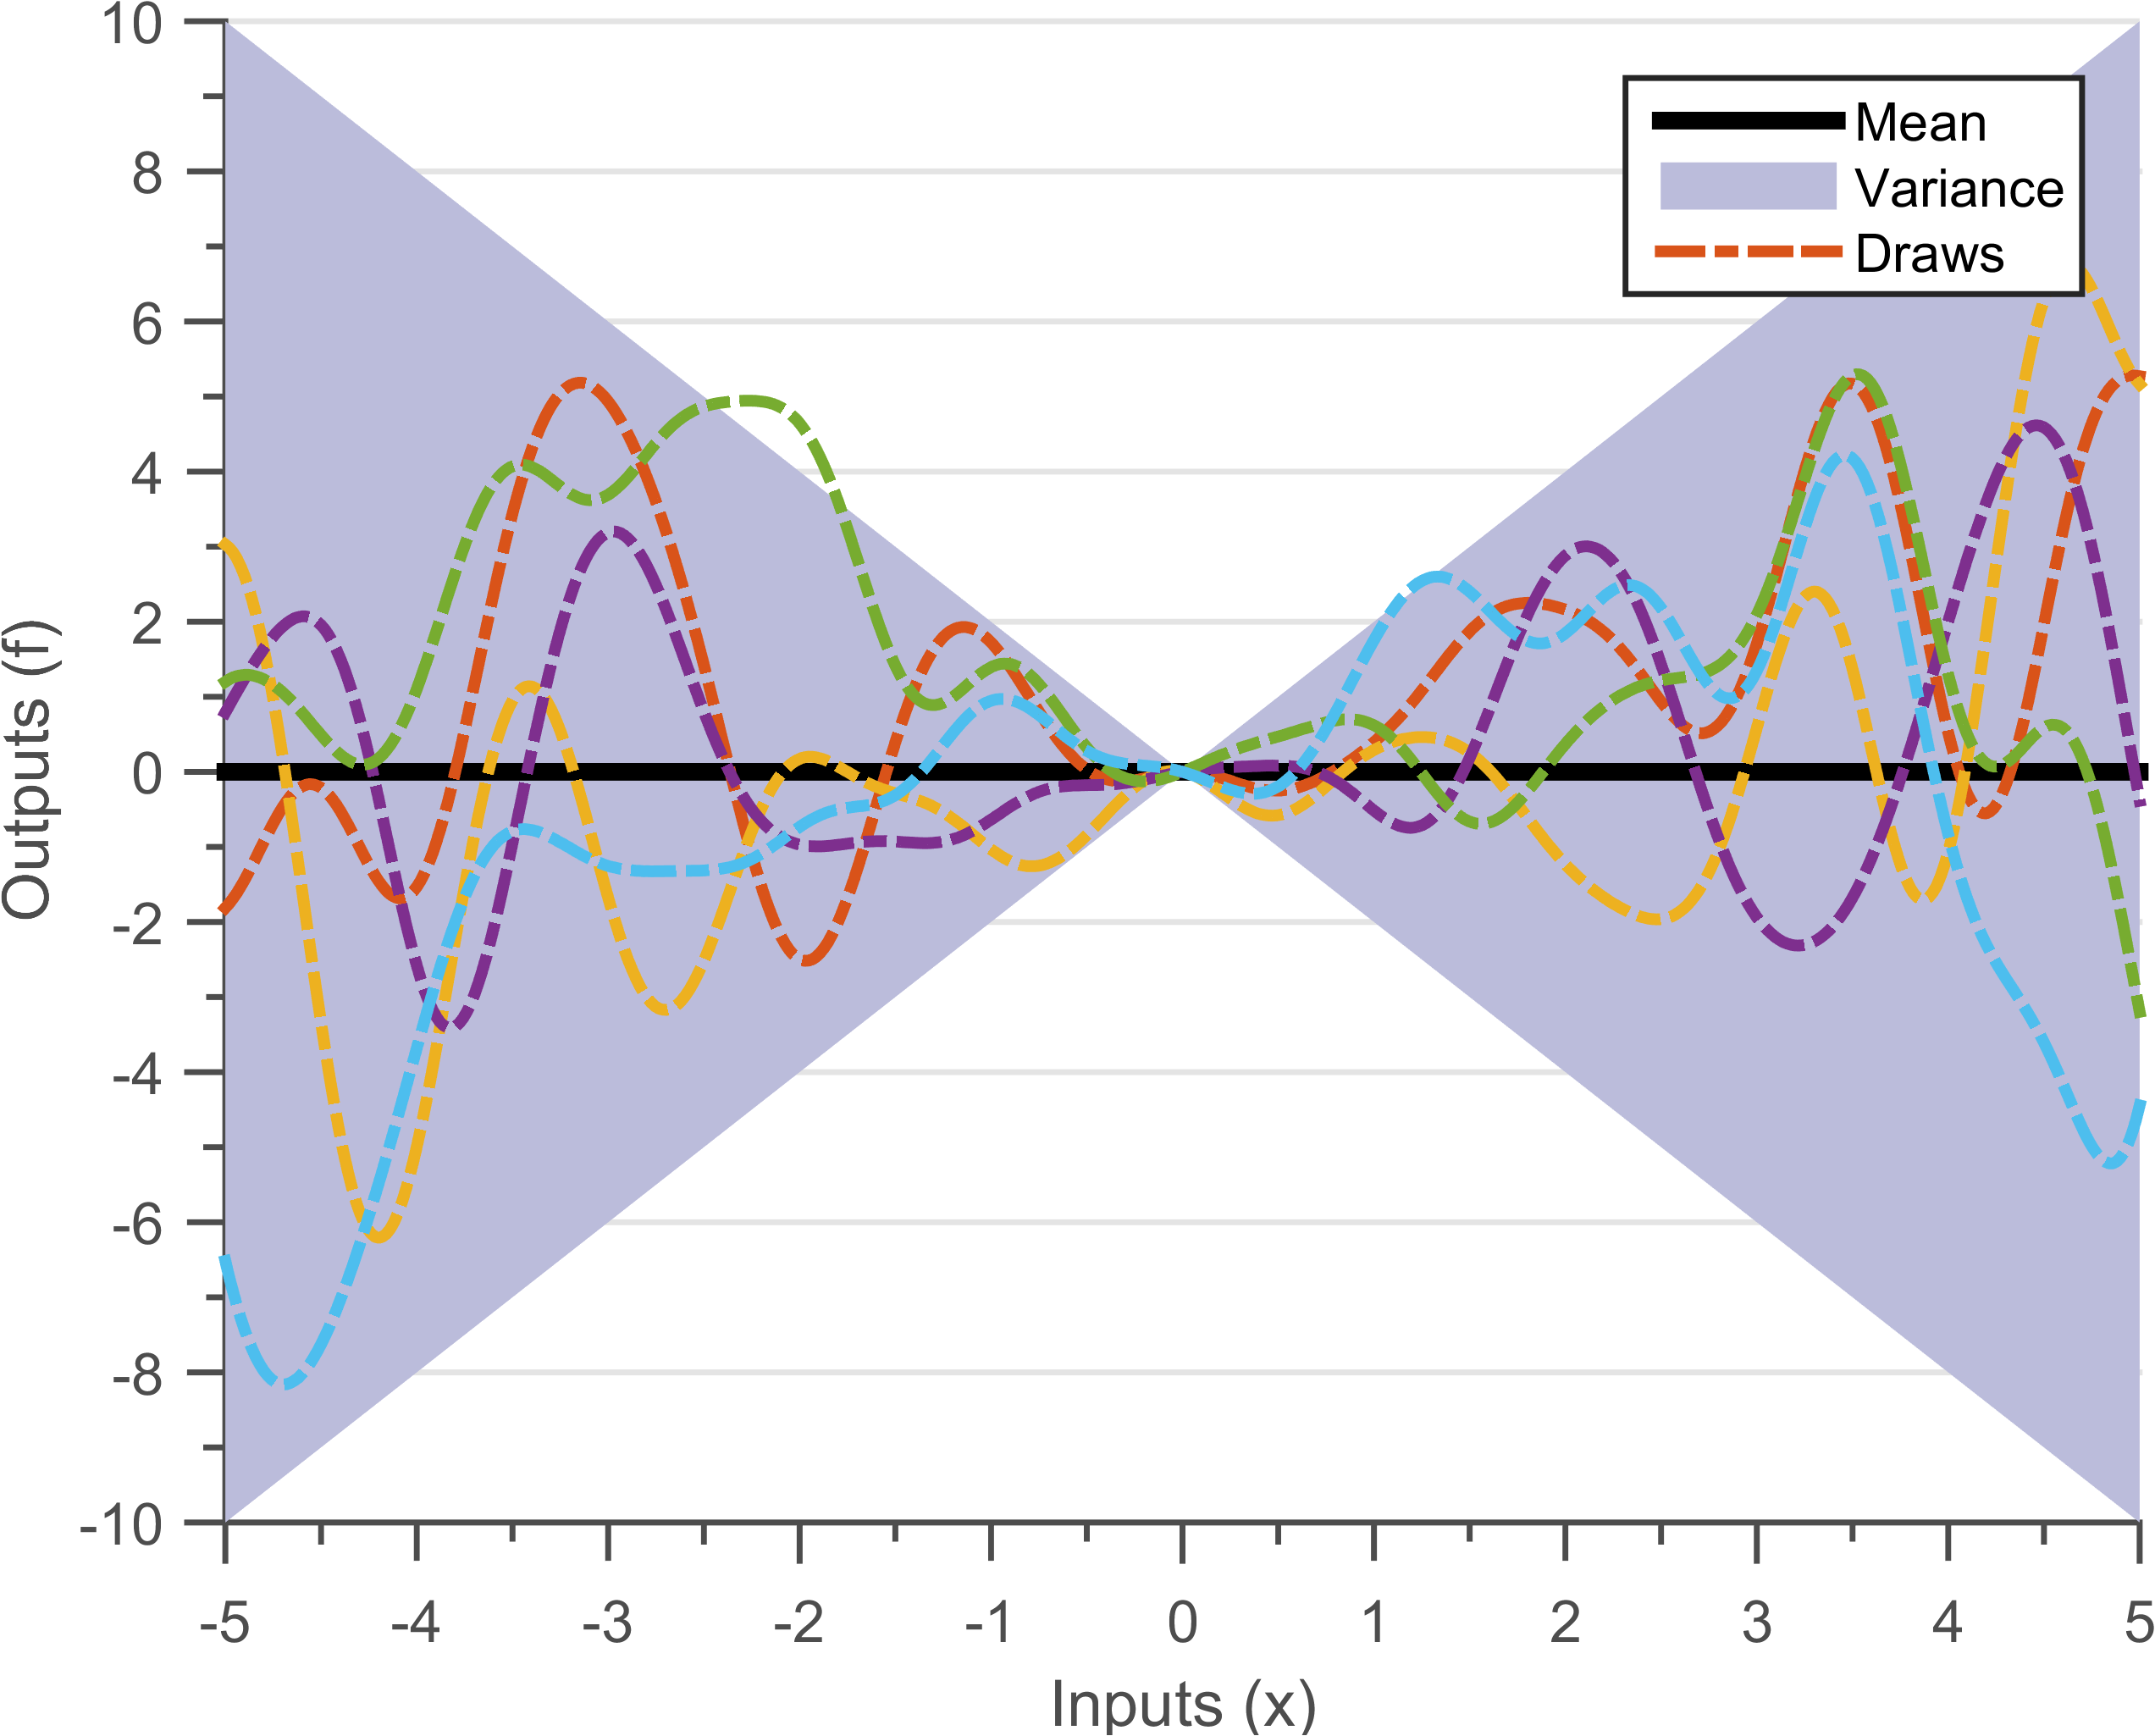
\includegraphics[width=0.45\textwidth]
        {images/part2/drawsMultiLinSE}
        \label{subFigPriorMultiLinSE}
  }\quad
\subfigure[{Draws from a GP prior with mean zero and kernel obtained by \textbf{adding} a Linear kernel with SE kernel. The hyper-parameters of the linear kernel are $w_{0}=0$ and $w_{1}=1$ while the hyper-parameters of the SE part are $\theta_{amplitude}=1$ and $\theta_{lengthScale}=1$. We see that the variance at $x=0$ goes to variance of SE kernel, since multiplication is an OR operation}]
  {
        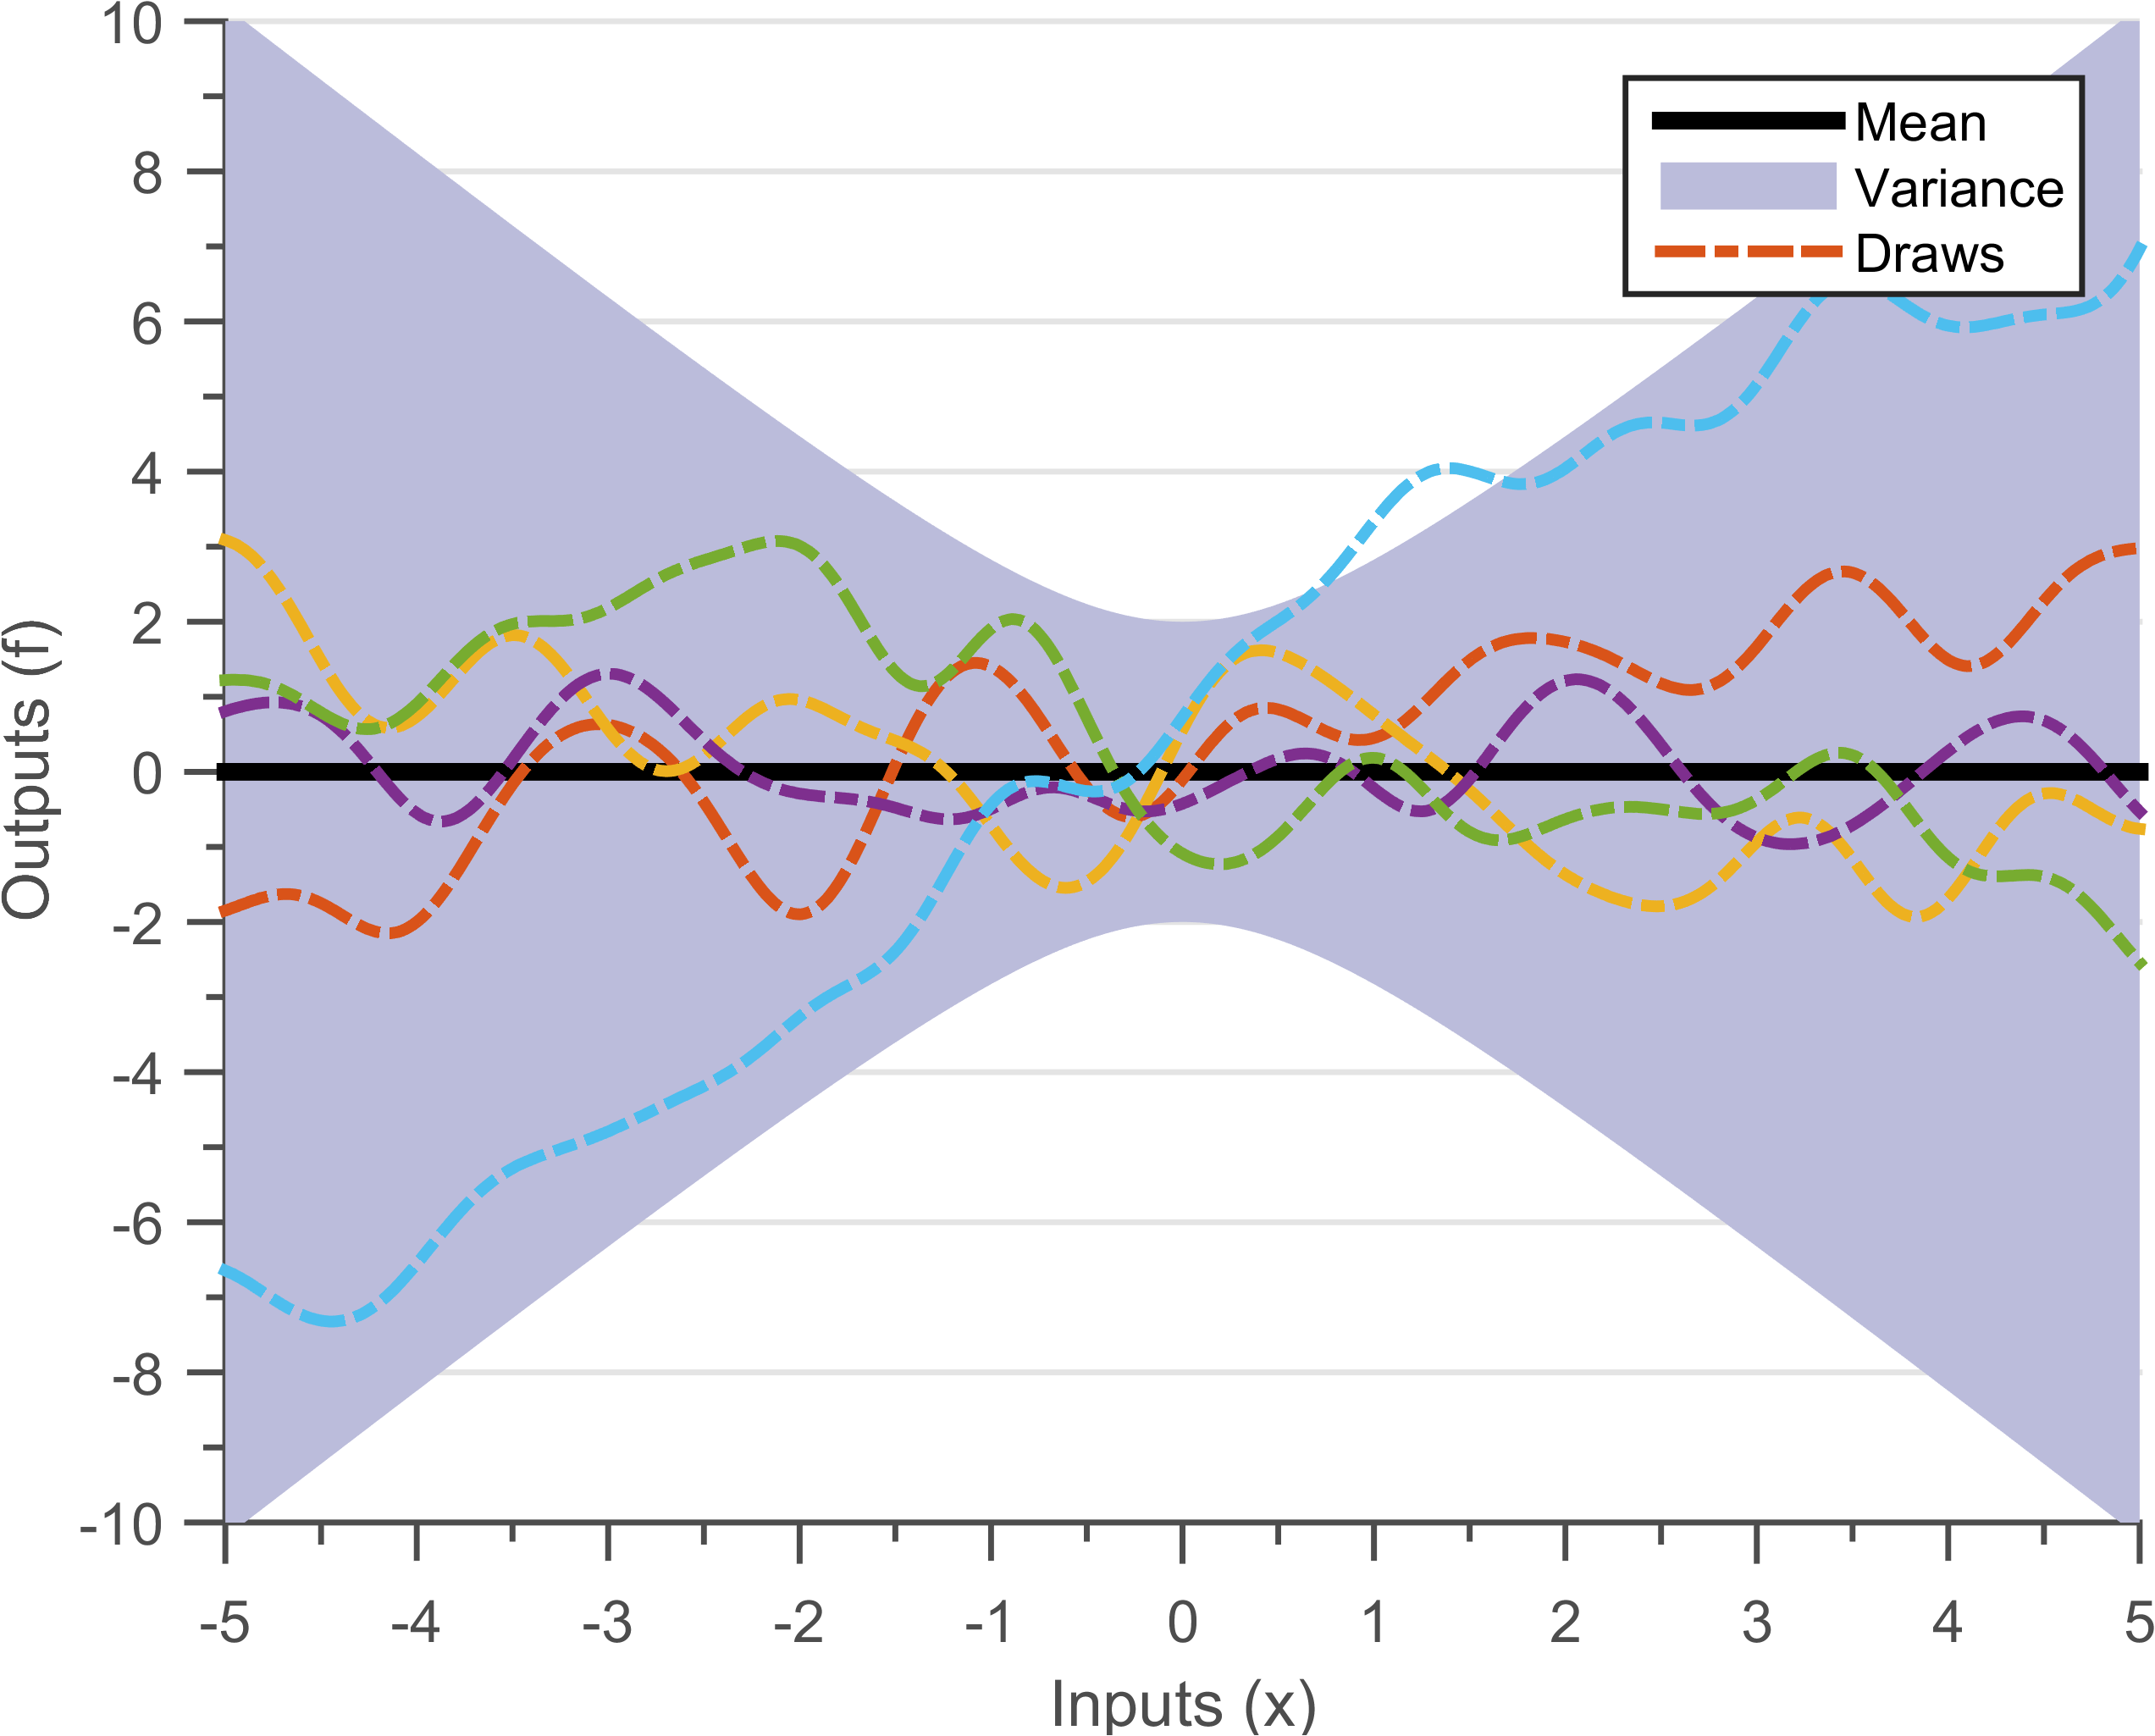
\includegraphics[width=0.45\textwidth]
        {images/part2/drawsSumLinSE}
        \label{subFigPriorAddLinSE}
  }\quad

       \caption{Random draws from combining a Linear and SE kernel. The solid black line defines the mean function, shaded blue region defines 95\% confidence interval (2$\sigma$) distance away from the mean. The dashed lines represent five functions drawn at random from a GP prior. Random functions drawn from a linear GP are linear.}
       \label{figPrior}
\end{figure}


\subsection{Adding Kernels} \label{subsecStructureKernelsAddingKernels}
Adding two kernels acts as an OR operator, this means that the resulting kernel will have high value if either of the two kernels have high value \cite{durrande2011additive}. 

Figure \ref{subFigPriorAddLinSE} shows the prior obtained after adding a Linear and a SE kernel. The hyper-parameters of the linear kernel are $w_{0}=0$ and $w_{1}=1$, this means that there is no intercept and $k_{Lin}(x_{1}, x_{2}) = x_{1}^Tx_{2}$. The hyper-parameters of the SE part are $\theta_{amplitude}=1$ and $\theta_{lengthScale}=1$, similar to figure \ref{subFigpriorDrawsSE}. 

\marginnote{\textsl{Adding Noise}}[1cm]
The Linear kernel discussed in section \ref{subSecCh4LinearKernel} is a sum of three covariance functions; a constant covariance ($\textcolor{red}{w_{0}}$), a linear covariance ($\textcolor{blue}{w_{1}x_{1}^T x_{2}}$) and a white noise covariance function ($\textcolor{green}{\sigma_{n}^2\delta_{xx'}}$) (equation \ref{eqDistributionOfLinearKernel}). Similarly, the noisy posterior case discussed in section \ref{figGPNoiseLessPosteriors} is a case of adding a SE kernel with a white noise kernel, a heteroscedastic\footnote{Noise depending on the inputs} noise model can be similarly created by adding several kernels together.

\begin{equation}\label{eqDistributionOfLinearKernel}
k(x_{1}, x_{2}) = \textcolor{red}{w_{0}} + \textcolor{blue}{w_{1} x_{1}^T x_{2}} + \textcolor{green}{\sigma_{n}^2\delta_{xx'}}
\end{equation}

An interesting consequence of adding kernels is that now we can decompose the result into additive parts. Suppose $k_{Sum}$ is a covariance function by adding $n$ covariance functions $k_{1}, k_{2}, \ldots, k_{n}$ (equation \ref{eqCh5AddingCovariances}), then the posterior mean and covariance can be written as equation \ref{eqCh5PosteriorSumMean} and \ref{eqCh5PosteriorSumVariance}. 

\begin{align}\label{eqCh5PosteriorSumMean}
\mathbf{E}[f(x) \mid \myMatrix{X}, \VEC{y}, k_{Sum}] = \sum_{i=1}^{n} \VEC{k_{i}(x_{*}X)}( \myMatrix{K_{Sum}(X, X)})^{-1} \VEC{y}
\end{align}

\begin{equation}\label{eqCh5PosteriorSumVariance}
Cov[f(x) \mid \myMatrix{X}, \VEC{y}, k_{Sum}] = \sum_{i=1}^{n} \left[ k_{i}(x_{*}x_{*}) - \VEC{k_{i}(x_{*}X)}( \myMatrix{K_{Sum}(X, X)} )^{-1} \VEC{k_{i}(Xx_{*})} \right ]
\end{equation}

Note that the precision matrix $( \myMatrix{K_{Sum}(X, X)} )^{-1}$ cannot be decomposed into its constituent covariance matrices. This is not an issue since this strategy is used to separate/discover individual effects in the data-set. For example, if we make a covariance function by adding a Linear kernel and an SE kernel, we can seperate the Linear part of the data-set from the non-linear part. 

\marginnote{\textsl{Discovering pattern}}[1cm]
This comes very handy while iteratively discovering structure in the data. One method to make an optimal covariance structure by hand is to iteratively add new kernels until the posterior error variance represents a white noise. \cite{Rasmussen2005} use a sum of several kernels to interpolate $CO_{2}$ content in the atmosphere through the years. \cite{durrande2013gaussian} use a sum of periodic kernels to detect which genes are responsible for the 24-hour cycle (\textit{circadian rhythm}) in \textit{arabidopsis} plant. \cite{duvenaud2013structure, lloyd2014automatic} propose to automatically detect pattern by adding new kernels, and using the BIC measure to find the optimal covariance structure. 

\subsection{Change-Point kernels}\label{subSecCh4CPKernel}
The CP kernel was introduced to recognize changes in regimes, and adapt the covariance function accordingly. They were initially introduced to identify change points in time-series modelling \cite{osborne2010bayesian, saatcci2010gaussian}. These kernels can be defined through addition and multiplication with sigmoidal functions (equation \ref{eqCh4SigmoidalFUnction}). 

\begin{align}
sigm(x, \theta) & = \frac{1}{\theta_{intensity} + e^{\theta_{changeLocation}-x}} \label{eqCh4SigmoidalFUnction} \\
k_{CP}(k_{1}, k_{2}, x_{1}, x_{2}) & = sigm(x_{1})k_{1}sigm(x_{2}) + (1-sigm(x_{1}))k_{2}(1-sigm(x_{2})) \label{eq:changePointKernel}
\end{align}

\marginnote{\textsl{Hyper-parameters}}[1cm]
The hyper-parameters of this kernel are the $\theta_{changeLocation}$ which determines the location of the change point, $\theta_{intensity}$ determine the intensity of change between the two patterns, and the hyper-parameters of covariance functions $k_{1}$ and $k_2$. Figure \ref{figdrawsCP} shows the randomly drawn functions from a CP kernel for varying values of $\theta_{intensity}$, where the regime changes from a Linear kernel to a SE kernel. The hyper-parameters of the linear kernel are $w_{0}=0$ and $w_{1}=1$, this means that there is no intercept and $k_{Lin}(x_{1}, x_{2}) = x_{1}^T x_{2}$. The hyper-parameters of the SE part are $\theta_{amplitude}=1$ and $\theta_{lengthScale}=1$, similar to figure \ref{subFigpriorDrawsSE}. We see that as the value of $\theta_{intensity}$ increases the regime change happens more rapidly, while if $\theta_{intensity}$ changes sign then the order of regime reverses.

\begin{figure*}[!ht]
  \centering
  \subfigure[{Draws from a GP prior with mean zero and CP kernel (equation \ref{eq:changePointKernel}) between a Linear and a SE kernel with $[\theta_{intensity}, \theta_{changeLocation}] = [1, 0]$.}]
  {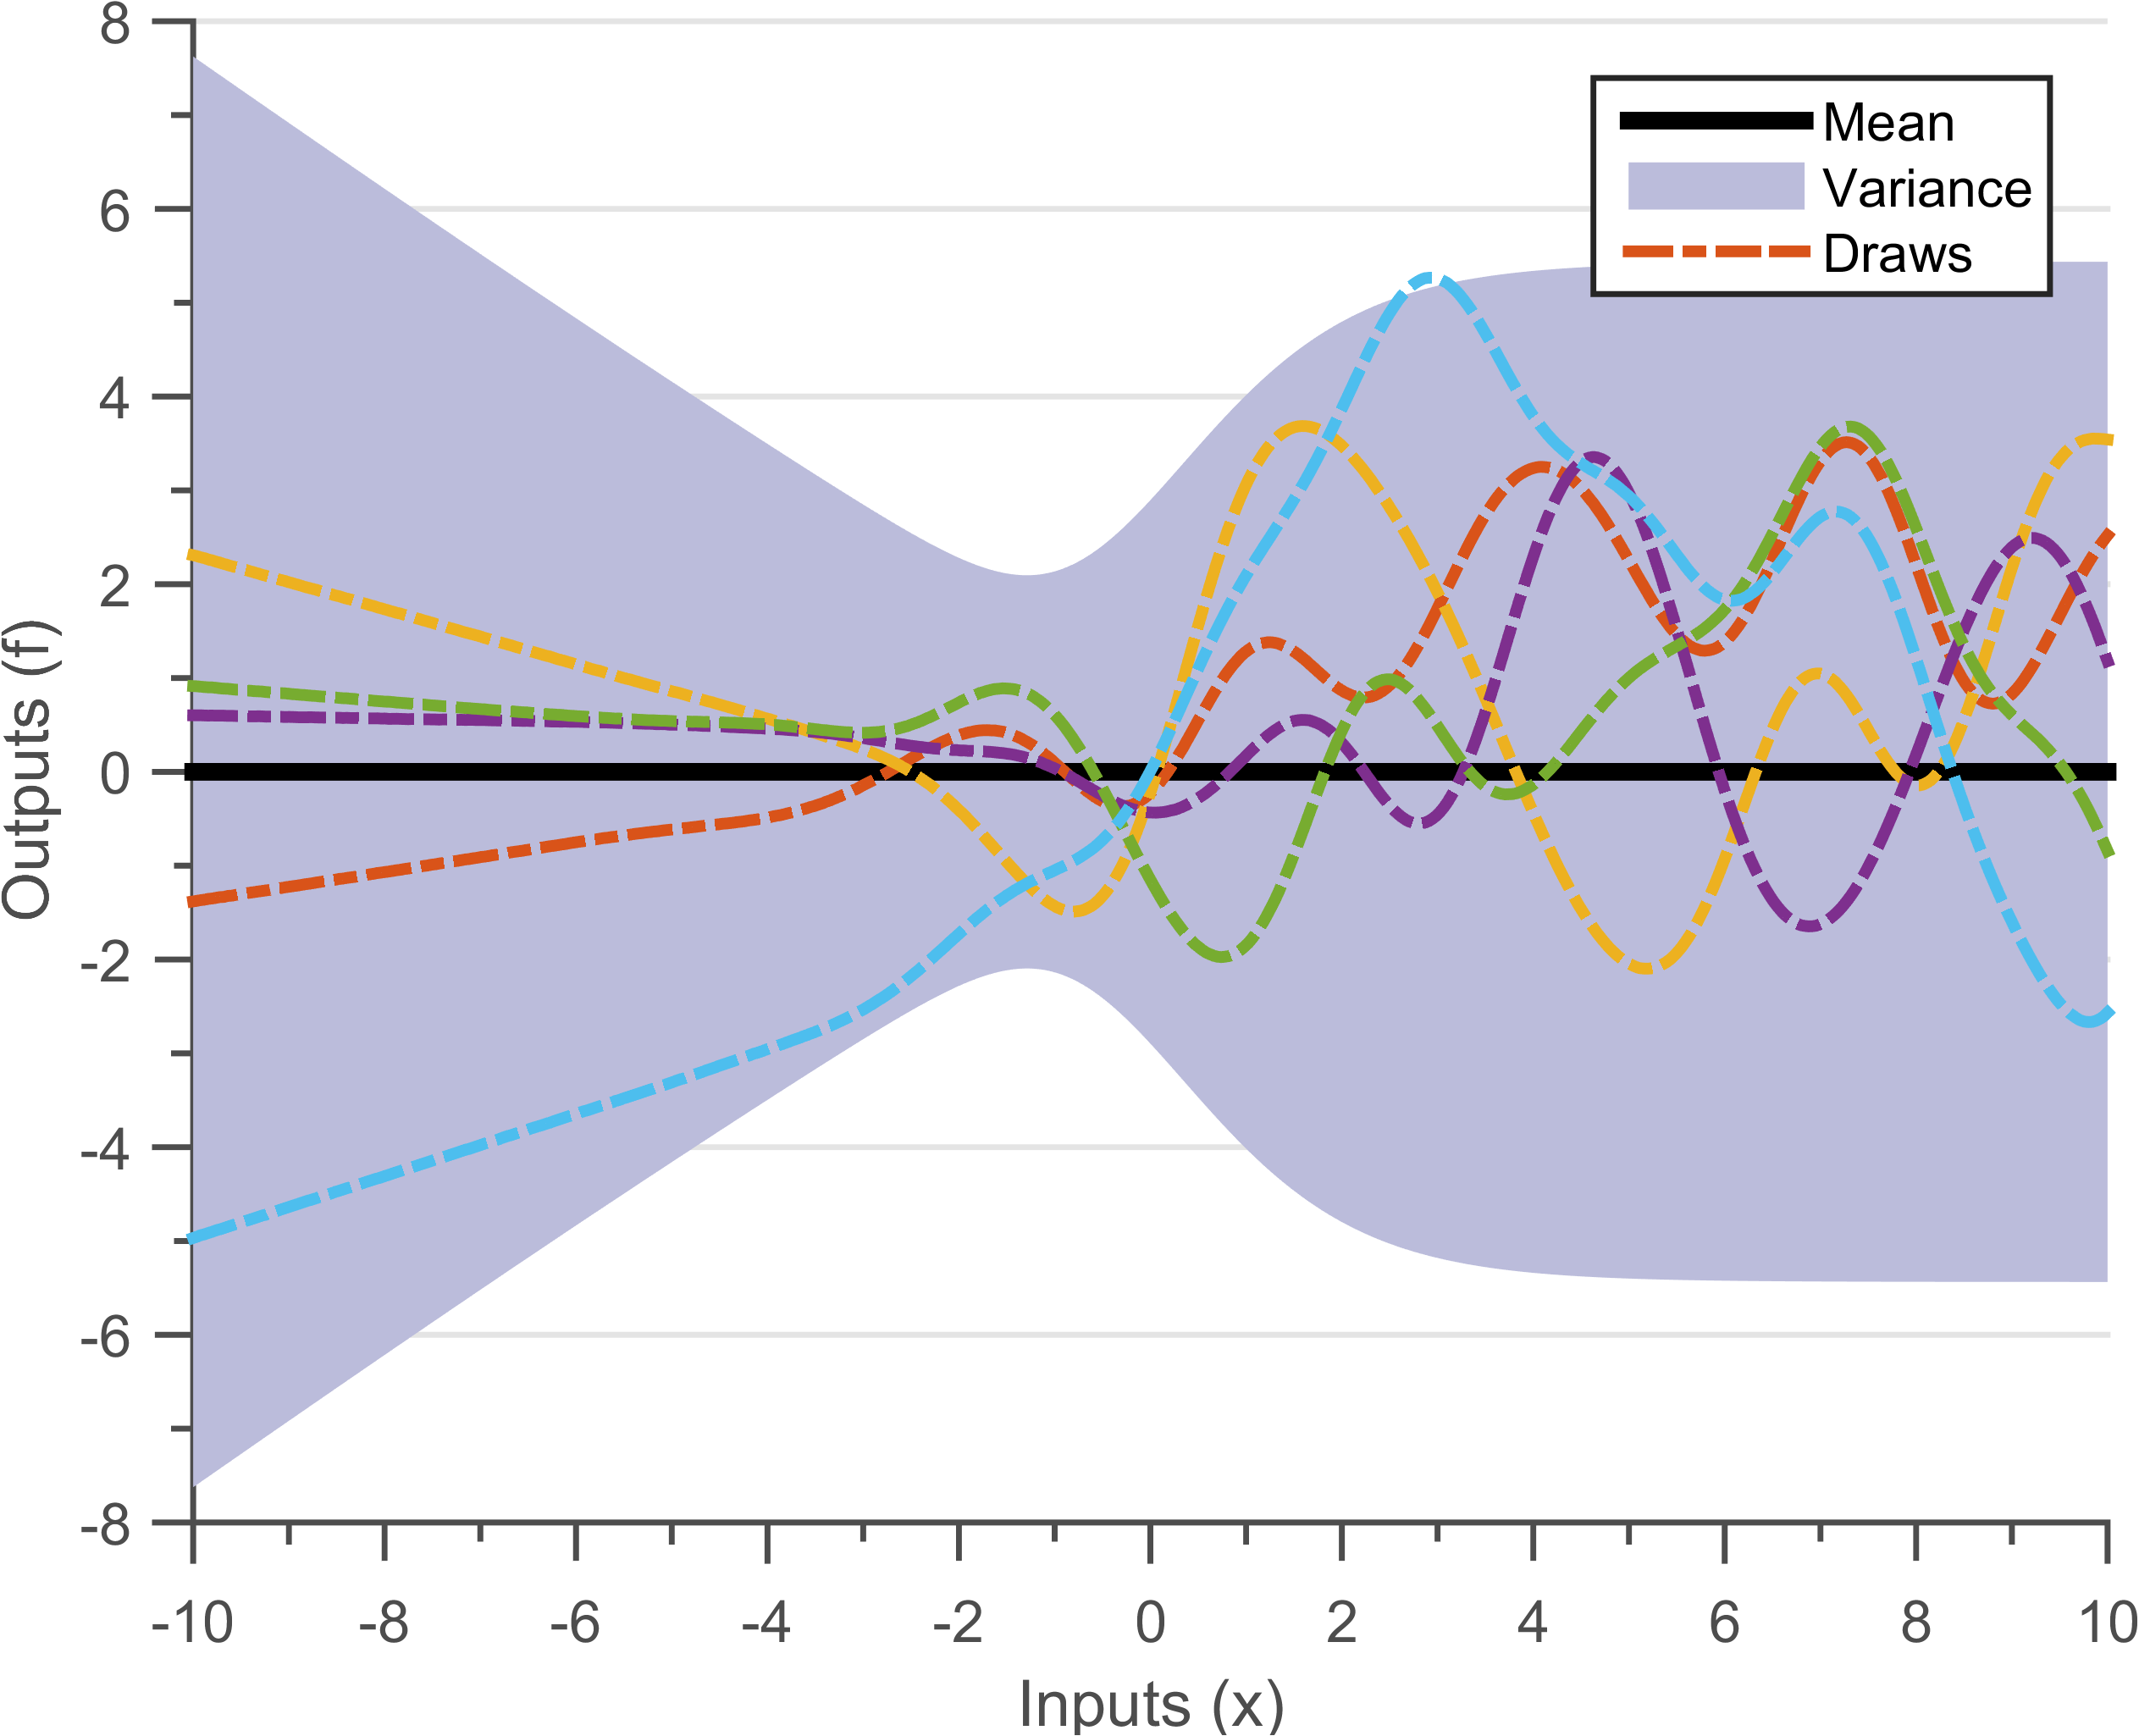
\includegraphics[width=0.29\textwidth]{images/part2/drawsCP1}\label{subfig:drawsCP1}}\quad
    \subfigure[{Draws from a GP prior with mean zero and CP kernel (equation \ref{eq:changePointKernel}) between a Linear and a SE kernel with $[\theta_{intensity}, \theta_{changeLocation}] = [10, 0]$. Notice if the value of $\theta_{intensity}$ increases then the change between two patterns becomes more significant.}]
  {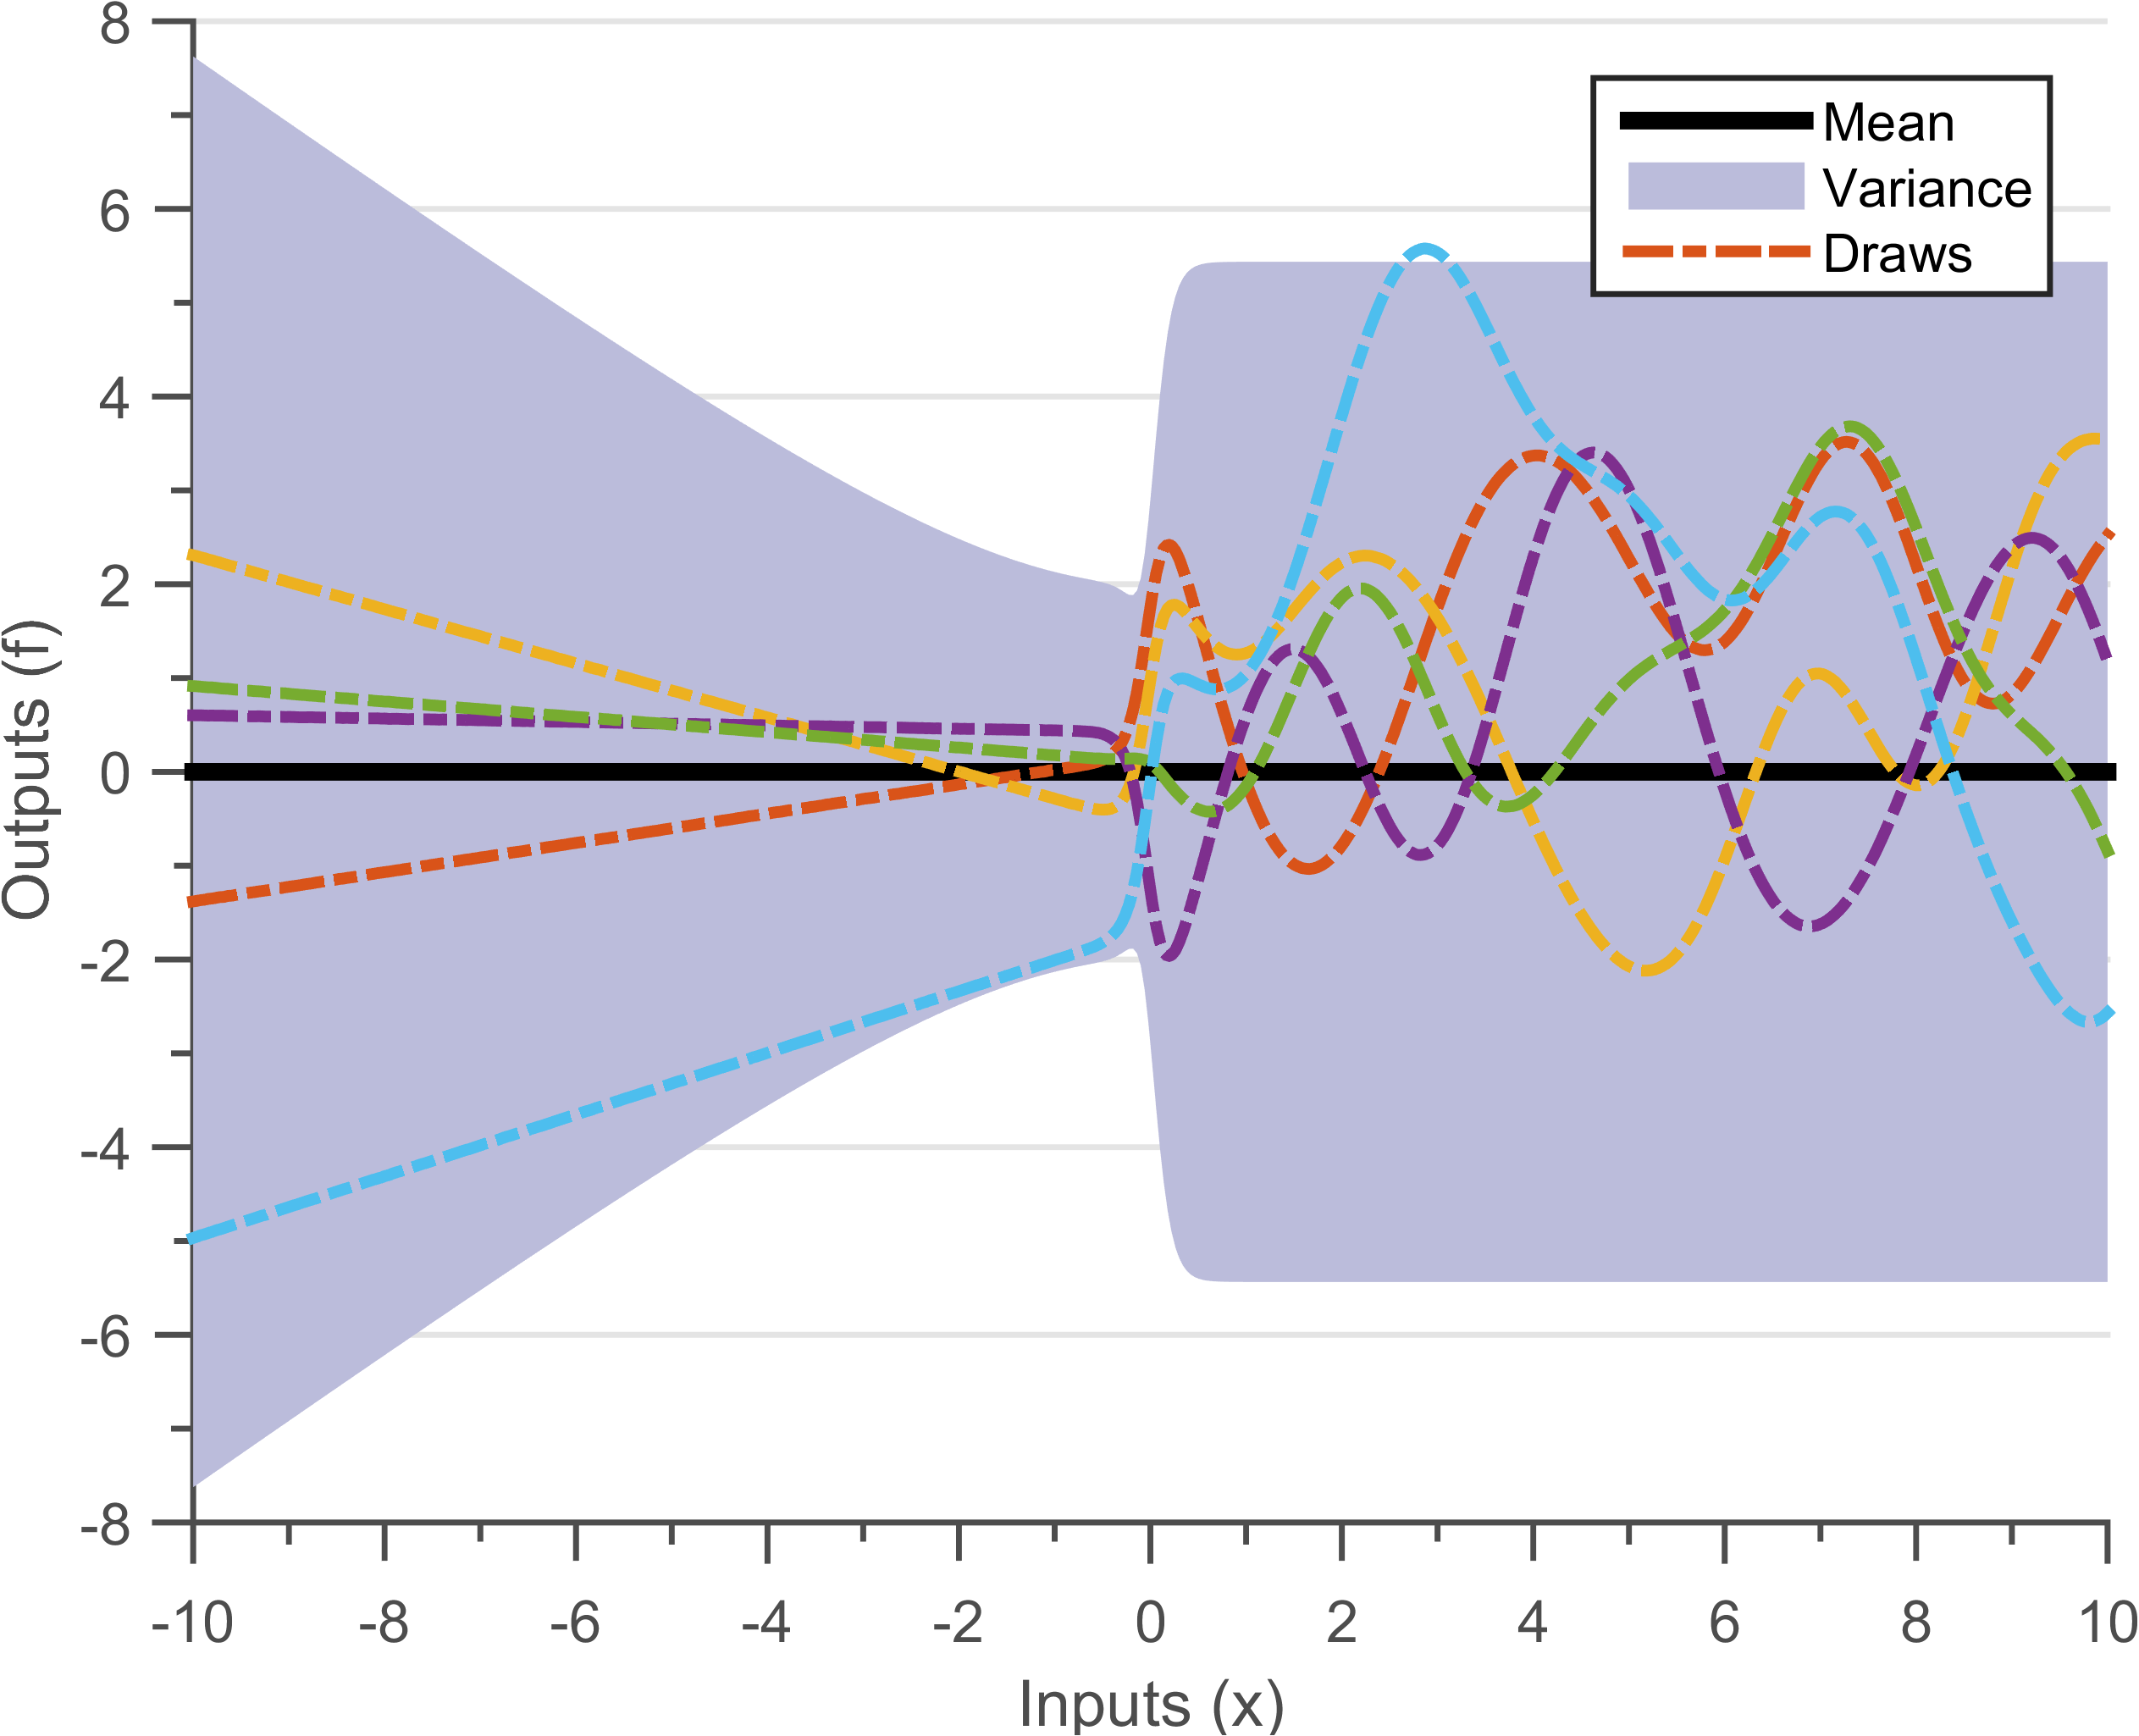
\includegraphics[width=0.29\textwidth]{images/part2/drawsCP10}\label{subfig:drawsCP10}}\quad
  \subfigure[{Draws from a GP prior with mean zero and CP kernel (equation \ref{eq:changePointKernel}) between a Linear and a SE kernel with $[\theta_{intensity}, \theta_{changeLocation}] = [-10, 0]$. Notice if the sign of $\theta_{intensity}$ changes then the order of kernels gets reversed.}]
  {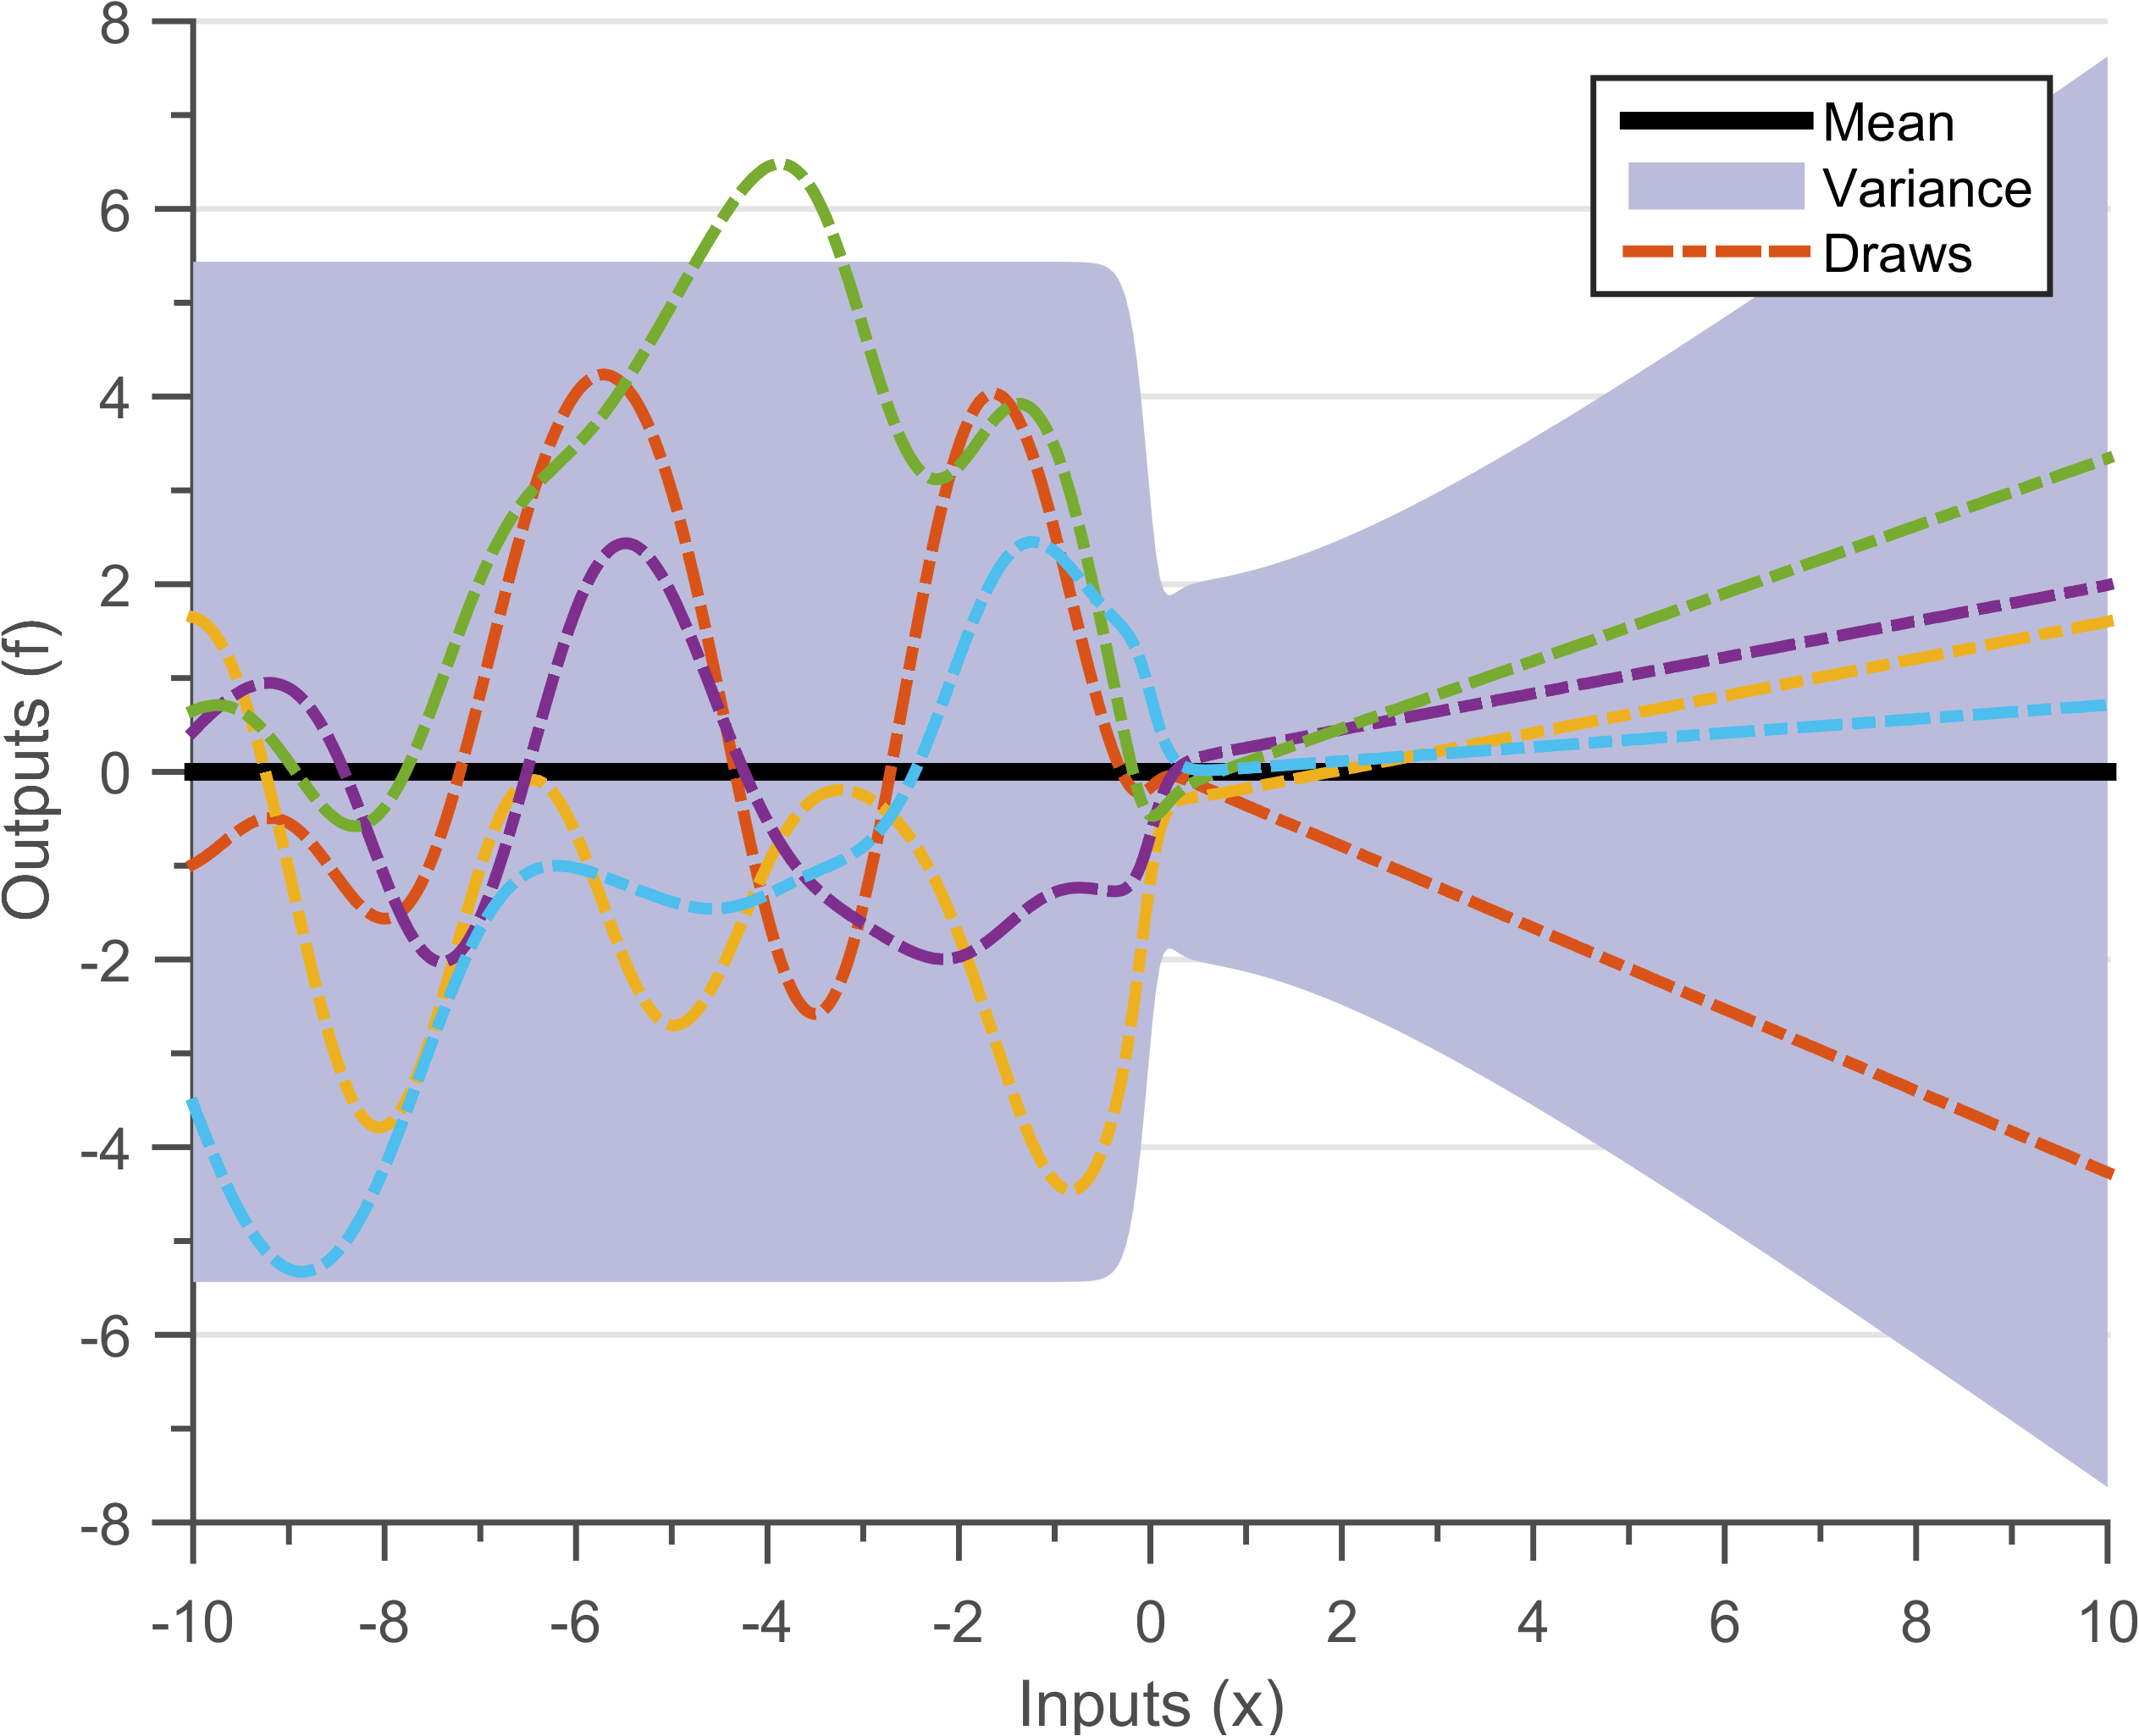
\includegraphics[width=0.29\textwidth]{images/part2/drawsCPMinus10}\label{subfig:drawsCPMinus10}}\quad
  \caption{Random draws by having a change-point between a Linear and SE kernel. The solid black line defines the mean function, shaded blue region defines 95\% confidence interval (2$\sigma$) distance away from the mean. The dashed lines represent five functions drawn at random from a GP prior. Random functions drawn from a linear GP are linear.}
  \label{figdrawsCP}
\end{figure*}

\subsection{Application: Identifying onset of non-linearity  using CP kernel}\label{subsubsecCh4ApplicationCP}
Several physical processes can be represented using a linear approximation in some part of their regime. This approximation is possible because the linear effects dominate in that part of the regime, but they eventually wear off and second and third order effects start becoming more powerful. 

\marginnote{\textsl{Linear assumption}}[1cm]
This basic assumption is used in making simple models in several domains; for example in a material during the elastic regime $Stress \propto Strain$ is a basic linear approximation. The proportionality constant between Stress and Strain is called Young's Modulus, which is unique for each material. When the elastic regime starts wearing off, non-linear behaviour called plasticity starts taking over and the approximation $Stress \propto Strain$ is not valid anymore. Similarly in aerodynamics, when characterizing a flow over an airfoil during the Linear regime  $ Lift \propto Angle Of Attack$, the airflow is attached on the airfoil during this regime. When the airflow starts separating from the airfoil the non-linear effects start dominating. 

\begin{mdframed}[hidealllines=true,backgroundcolor=blue!20]
\marginnote{\textsl{Contribution}}[1cm]
The value of these basic physical parameters such as slope (eg. Young's Modulus, coefficient of lift) and location of change in regime (eg. start of plasticity and separation of flow) are progressively fed into further simulations. Generally, the slope and location of change points are evaluated using engineering judgment, this is a slow and costly process. We propose to estimate the slope and location of change-point automatically using a GP with CP kernel. Using the CP kernel which transitions from linear domain (linear kernel) to non-linear domain (SE kernel), prior information of the transition is encoded in the kernel structure. 

% \textbf{Correct the units in aluminium}

We perform our experiments on openly available Stress and Strain data of Aluminum Alloy 6061 \cite{kaufman1999properties} and Lift and Angle data of NACA 0012 airfoil\footnote{Airfoil data from: \url{http://airfoiltools.com/airfoil/details?airfoil=n0012-il}}. To estimate the CP hyper-parameters, we again perform a 10-fold cross validation. The data-set will be randomly partitioned into 10 subsets containing an equal number of points. Of the 10 subsets, a single subset is retained as the test data-set, and the remaining 9 (10 - 1) subsets are used as training data. The cross-validation process is then repeated 10 folds, with each of the k subsets used exactly once as the validation data. The marginal-likelihood is optimized for each of the training data-set and location of change-point and slope of the linear regime is noted. We then compare their average with the values available in the literature. 
\end{mdframed}


Table \ref{tabComparisonOfYoungModulus6061Data} shows the results of physical parameters for AL 6061 when calculated using change-point kernel vs that available in the literature. We can observe that the change-point automatically predicts the correct values of Young's Modulus and start of non-linearity.


\begin{table}[!ht]
    \centering
\begin{tabular}{|l|l|l|}
  \hline
    & Change-point & Literature \\
  \hline 
  \hline
Young's Modulus (GPa) &  68.5 & 68.9\\
Start of plasticity  & 0.94\% & 0.95\%\\
   \hline
\end{tabular}
\caption{Comparison of Young's Modulus for Al 6061 data-set}
  \label{tabComparisonOfYoungModulus6061Data}
\end{table}

\marginnote{\textsl{Figure \ref{figPosteriorChangePointKernel}}}[1cm]
Figure \ref{figPosteriorChangePointKernel} shows the posterior predictions when using the CP kernel. Figure \ref{subfig:clAlphaCovCP} is the posterior distribution for the case of NACA 0012 airfoil, the Linear and SE regimes are plotted independently. Figure \ref{subfig:stressStraincovCPPlot} shows the posterior distribution for the case of AL 6061. We can observe that the algorithm predicts a CP for the data-set, this is the point where the non-linear effects start dominating. 

The marginal likelihood of a change-point kernel has many local minimas, there is a local minimum at every observation point. This is because the kernel puts a non-linear regime at every observation point, hence a global optimizer should be used for optimization. The results of this study were be presented in the SIAM Uncertainty Quantification 2016 Conference \cite{chiplunkar:hal-01555401}.
\marginnote{\textsl{Multi-modality}}[-1cm]

\begin{figure}[!ht]
  \centering
    \subfigure[{Posterior distribution for the case of NACA 0012 airfoil, the Linear and SE regimes are plotted independently.}]
	    {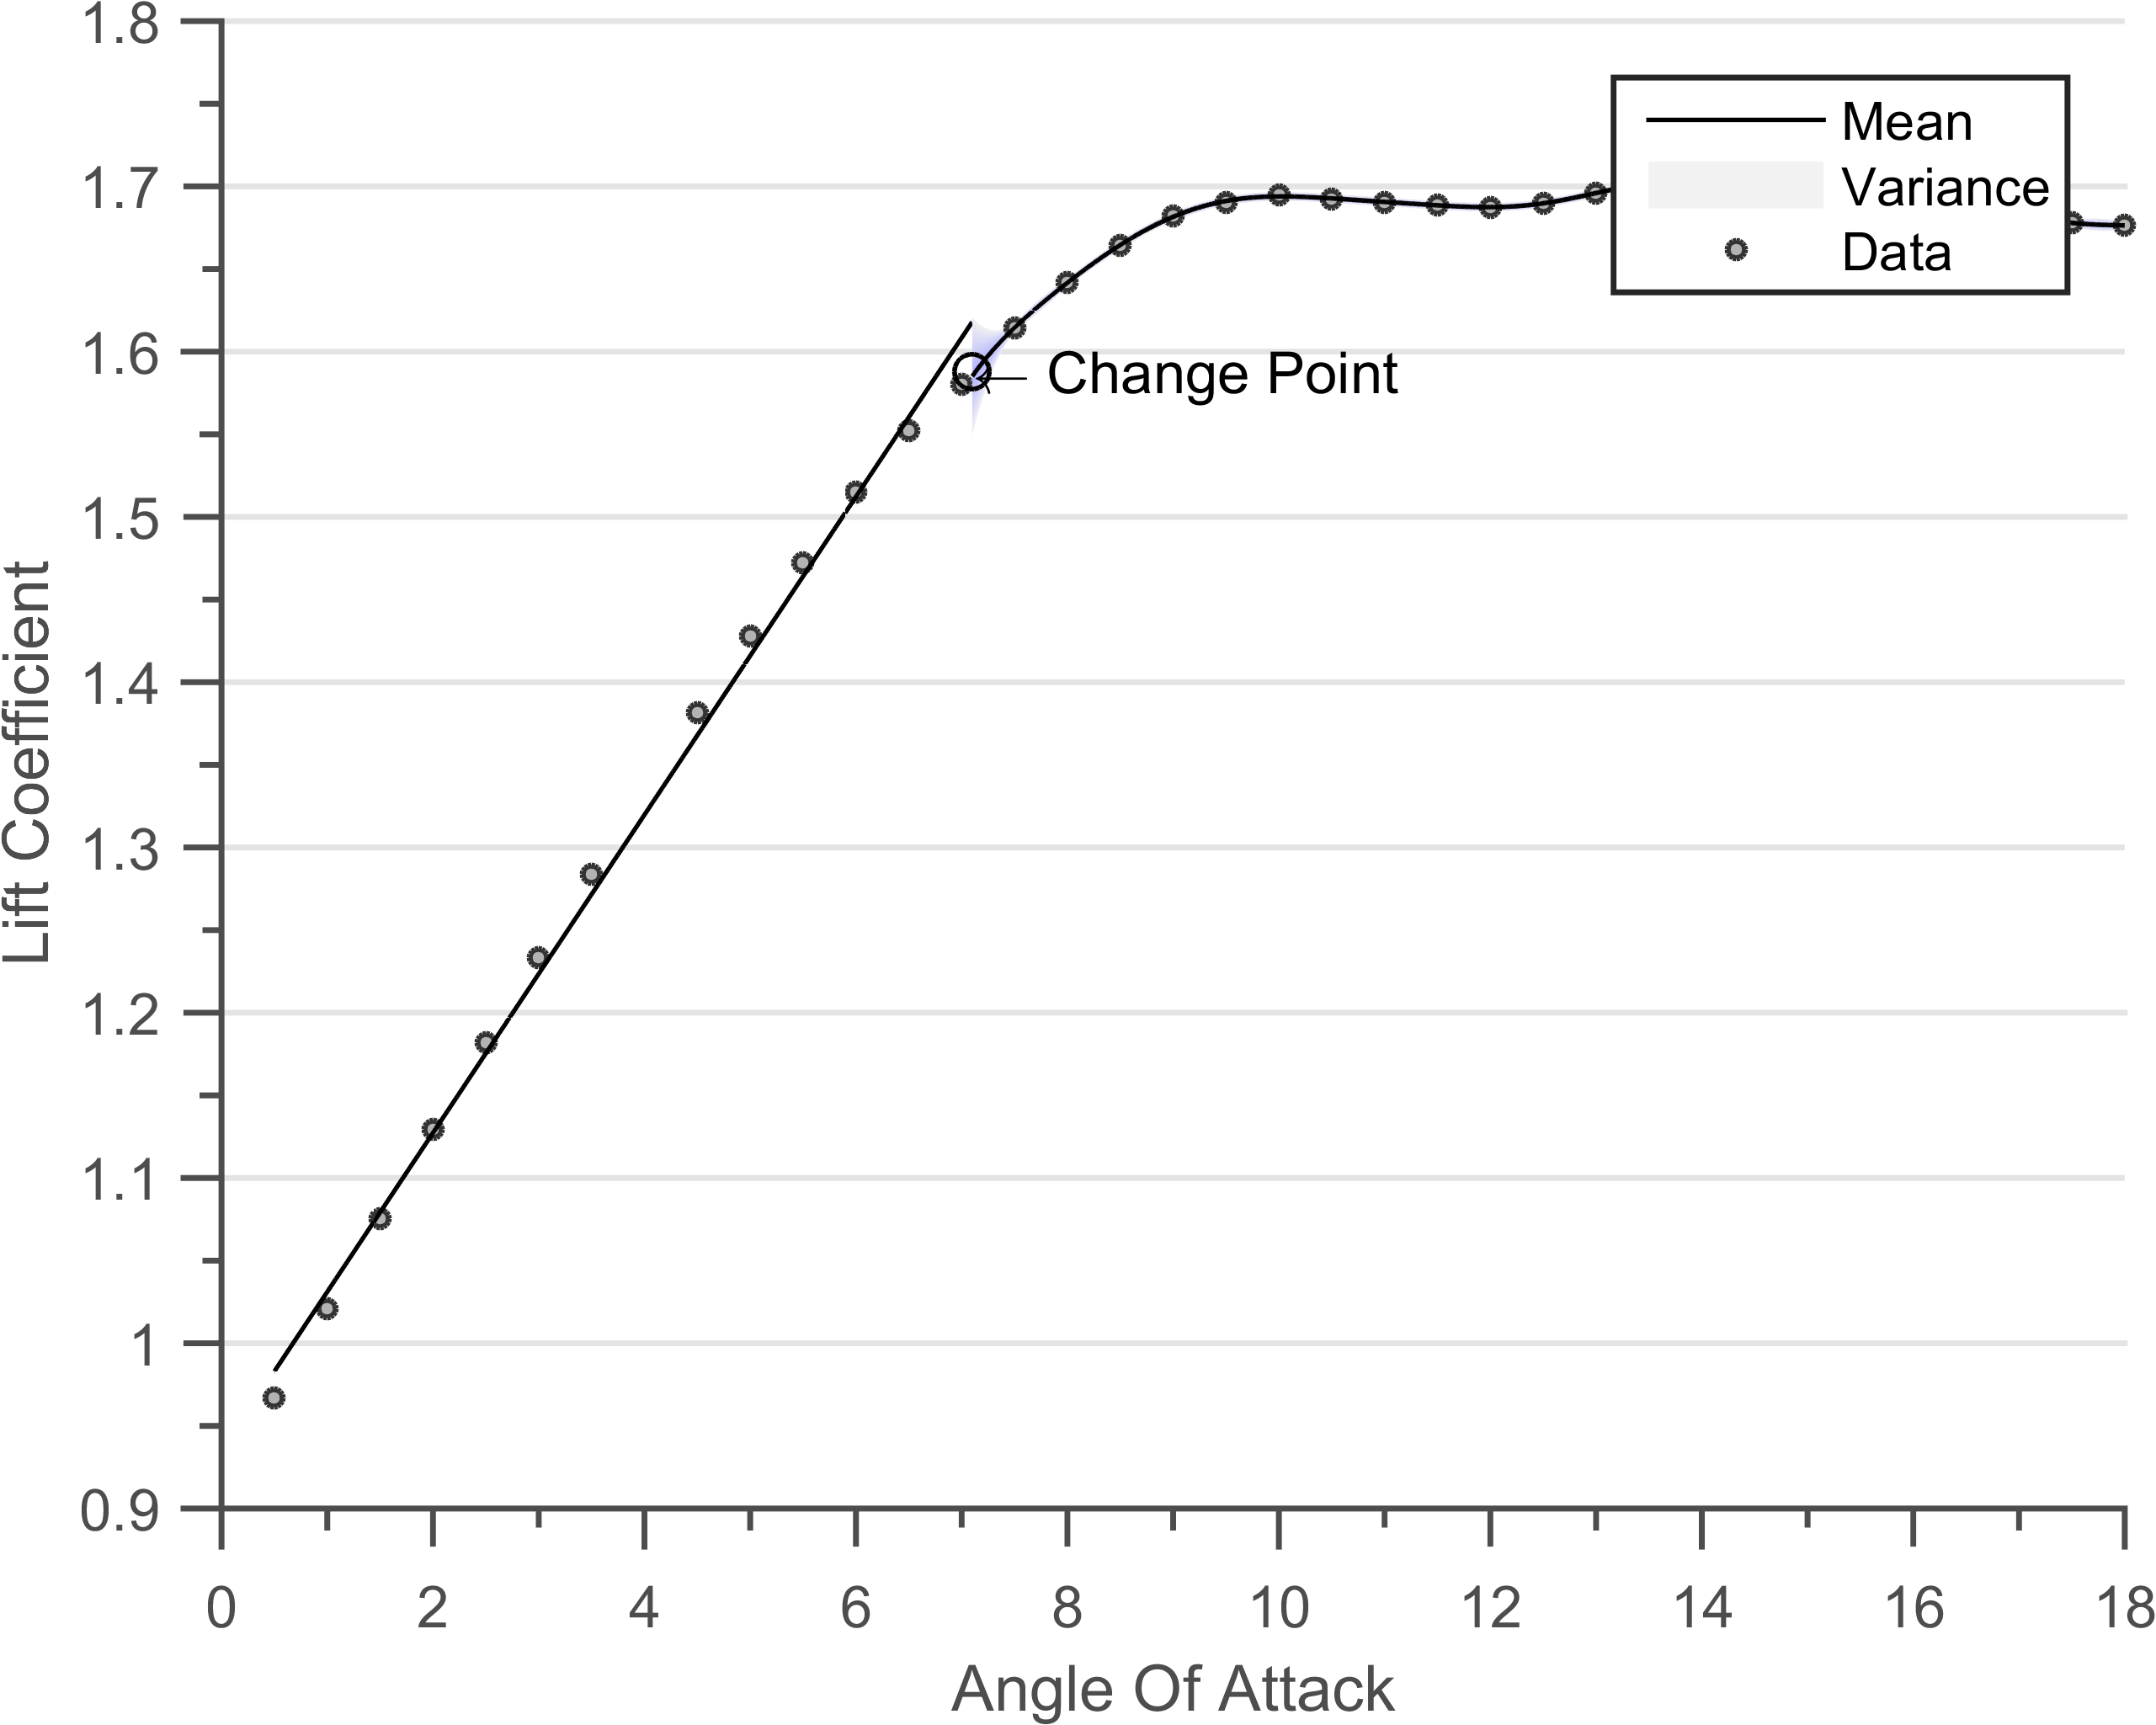
\includegraphics[width=0.45\textwidth]{images/part2/clAlphaCovCP}\label{subfig:clAlphaCovCP}}\quad
    \subfigure[{Posterior distribution for the case of AL 6061 alloy, the Linear and SE regimes are plotted independently.}]
	    {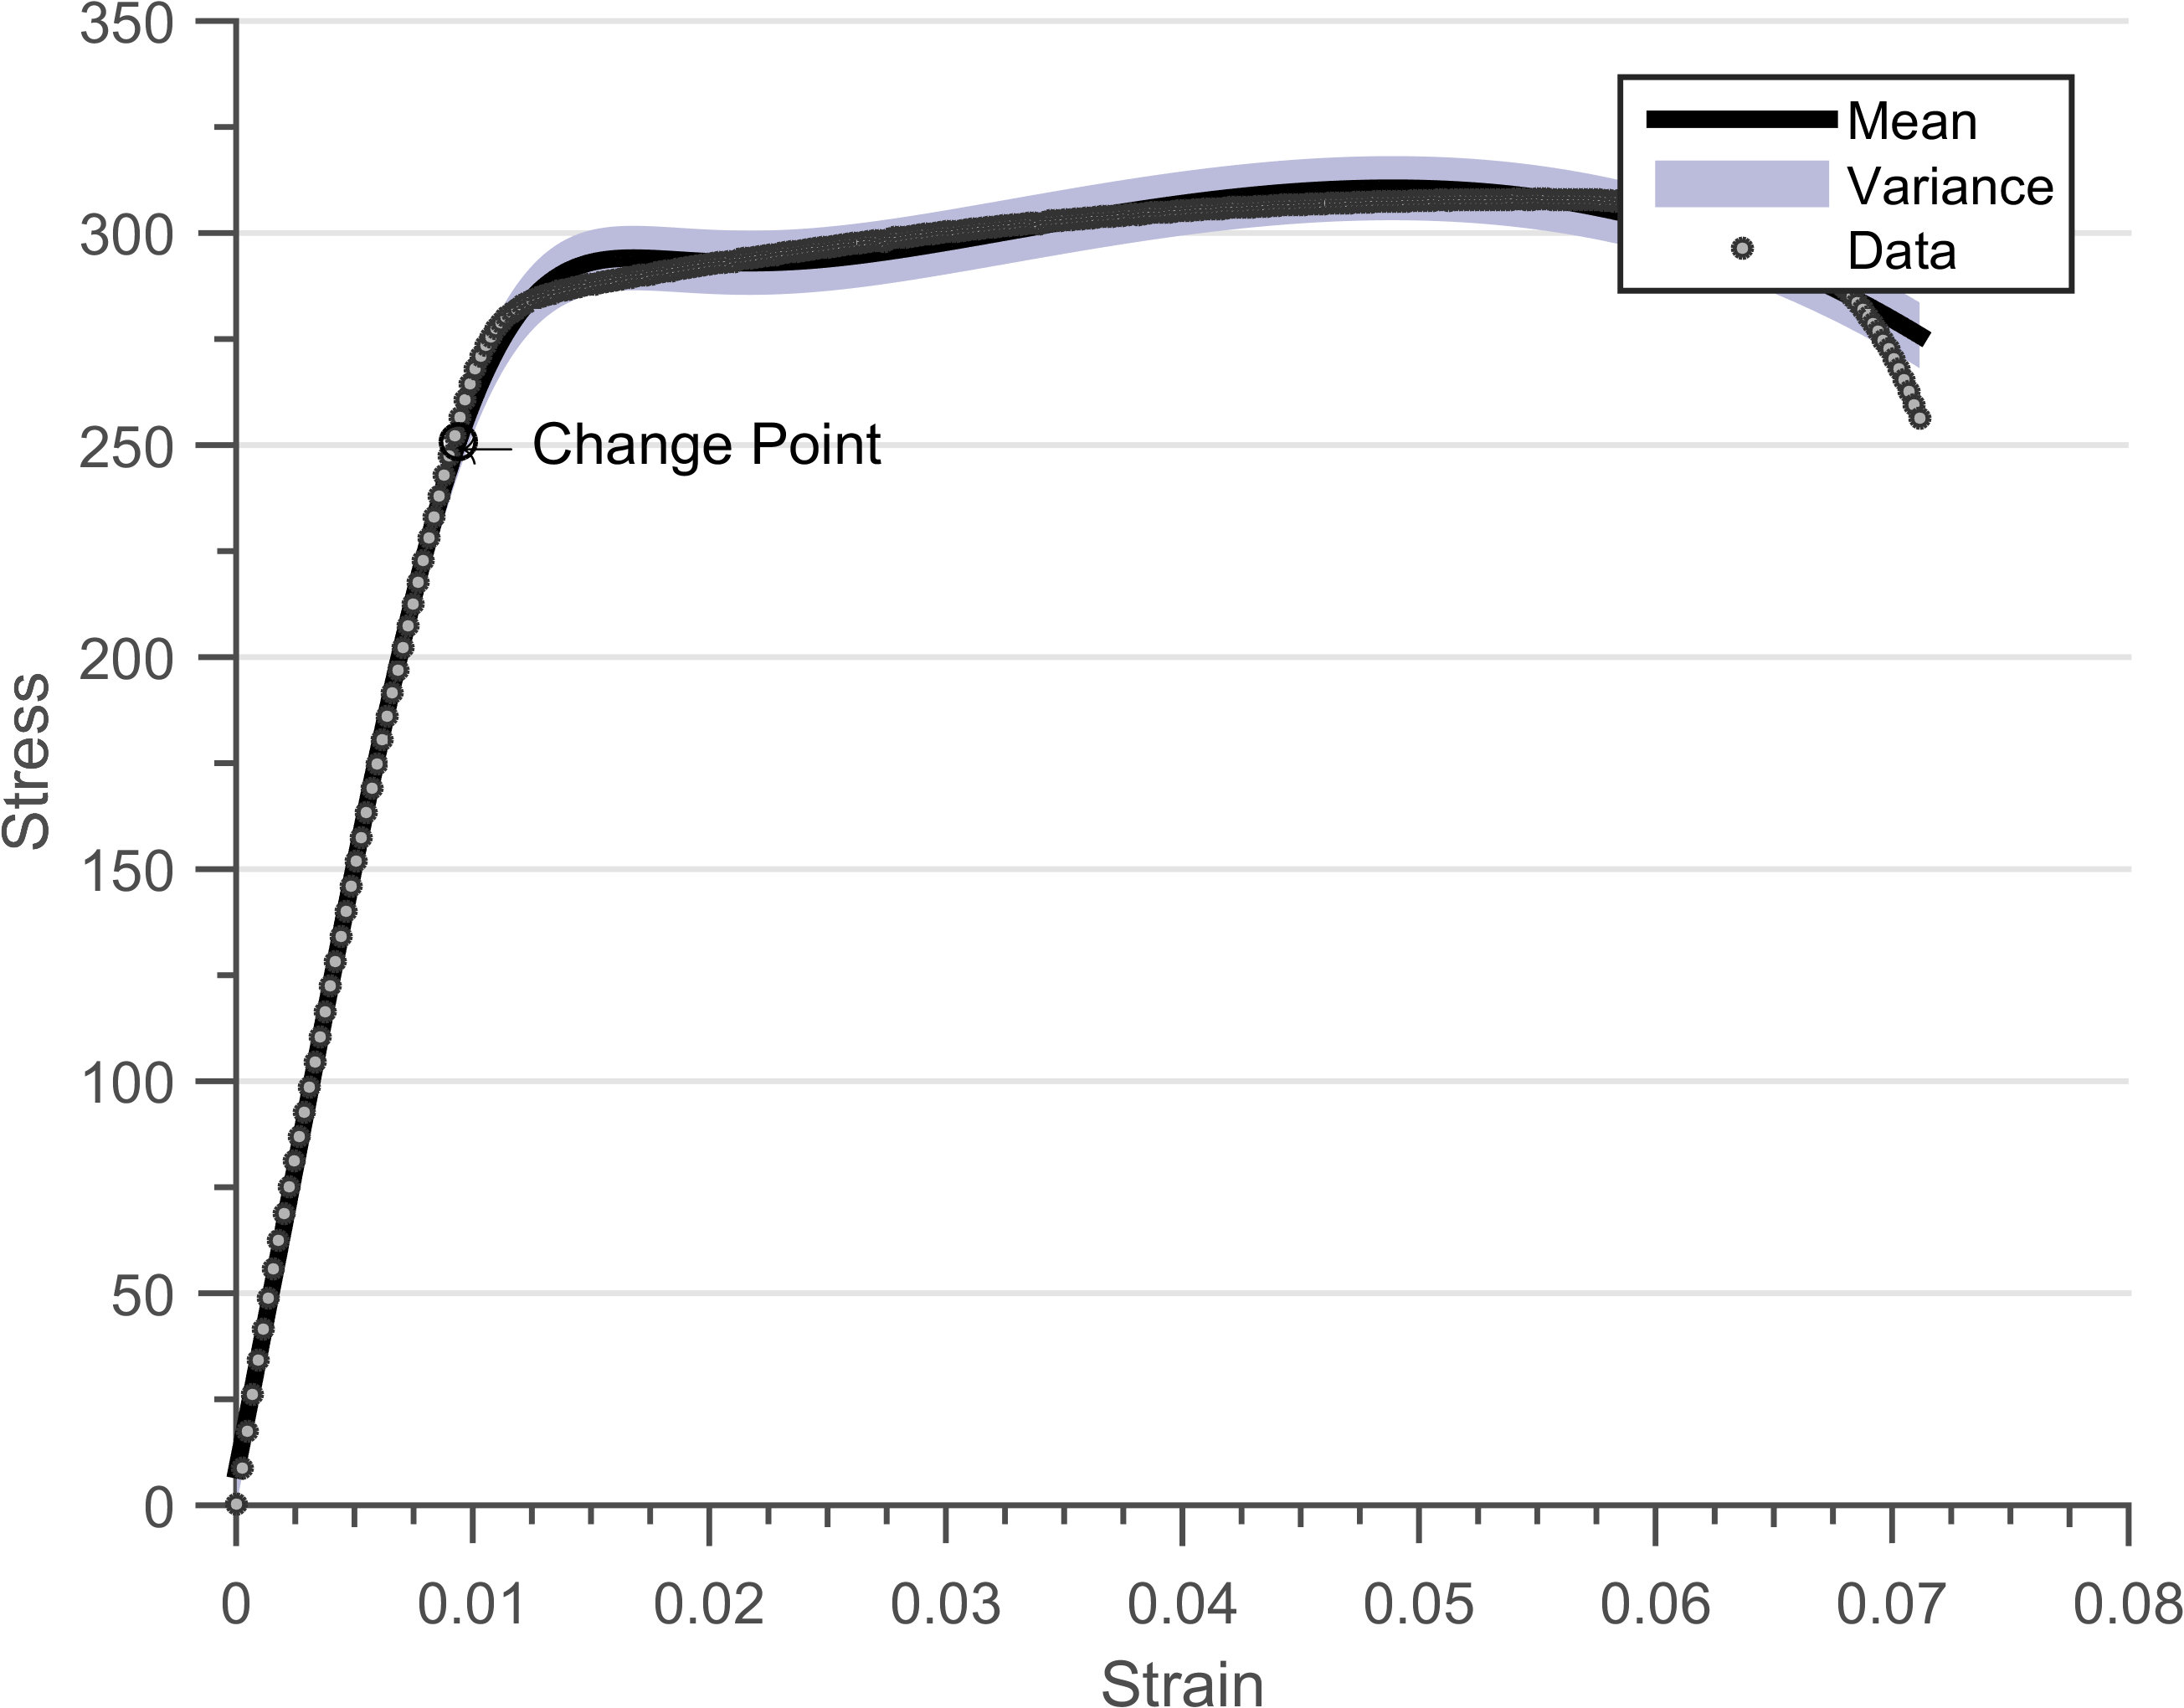
\includegraphics[width=0.45\textwidth]{images/part2/stressStraincovCPPlot}\label{subfig:stressStraincovCPPlot}}
        \caption{Estimation of linear regimes using a change-point kernels}
        \label{figPosteriorChangePointKernel}
\end{figure}


\section{Multi-dimensional kernels}\label{secMultiDimensionalKernels}
In this section we develop intuitions on how to build kernels for higher-dimensional inputs. This section demonstrates what happens when we add or multiply kernels across dimensions (equation \ref{eqCh5AddingAcrossDimensionsCovariances} and \ref{eqCh5MultiplyingAcrossDimensionsCovariances}), while also providing kernels on how to perform sensitivity analysis or to encode lower-dimensional structure (equation \ref{eqCh5ComposedCovariances}). We then apply the multi-dimensional covariance function to interpolate aerodynamic pressure (section \ref{subecInterpolationOfAerodynamicPressures}), comparing the accuracy of GP interpolation with common POD technique \cite{oatao18004}. 

\subsection{Adding across dimensions}
Consider an input data-set which is multi-dimensional $\VEC{x} \in \mathbb{R}^{D_{inputs}}$. A simple additive kernel can be constructed by adding the kernels for individual dimensions \cite{hastie1990generalized}. This operation encodes the information that added dimensions are independent of each other (equation \ref{eq:SESum}). 

\begin{equation}\label{eq:SESum}
k(\VEC{d}, \VEC{\theta}) = \sum_{i=1}^{D_{inputs}} (\theta_{amplitude}^{i})^2 exp\left [ -\frac{(d^{i})^2}{2(\theta_{lengthScale}^{i})^2} \right ]
\end{equation}

Here, $d^{i} = x^{i}_{1} - x^{i}_{2}$ is the distance between two input points at the $i^{th}$ dimension. Figure \ref{subFigdrawsSumMultiDimensional} is a randomly drawn function after adding two SE kernels, the hyper-parameters of both the SE kernels are $\theta_{amplitude}=1$ and $\theta_{lengthscale}=0.2$. 

\subsection{Multiplying across dimensions}
If we want to include interactions between two dimensions then their kernels can be multiplied together (equation \ref{eqCh5MultiplyingAcrossDimensionsCovariances}). A kernel which allows for interaction between all the possible $D_{inputs}$-dimensions can be constructed by multiplying all kernels for all the dimensions. The multi-dimensional Automatic Relevance Determination (ARD) kernel (equation \ref{eq:SEARD}) can be seen as a multiplication of several one-dimensional kernels with different length-scales \cite{Rasmussen2005}. It is called ARD because the value of length-scale determines which dimensions are more relevant.

\begin{equation}\label{eq:SEARD}
k(\VEC{d}, \VEC{\theta}) = (\theta_{amplitude})^2 \prod_{i=1}^{D_{inputs}}  exp\left [ -\frac{(d^{i})^2}{2(\theta_{lengthScale}^{i})^2} \right ]
\end{equation}

Figure \ref{subFigdrawsProdMultiDimensional} is obtained after multiplying 2 SE kernels, the hyper-parameters of both the SE kernels are $\theta_{amplitude}=1$ and $\theta_{lengthscale}=0.2$ 

\begin{figure}[!ht]
  \centering
    \subfigure[{Random draw from a 2 dimensional prior obtained after \textbf{multiplying} two SE kernels. The hyper-parameters of both the SE kernels are $\theta_{amplitude}=1$ and $\theta_{lengthscale}=0.2$}]
  {
        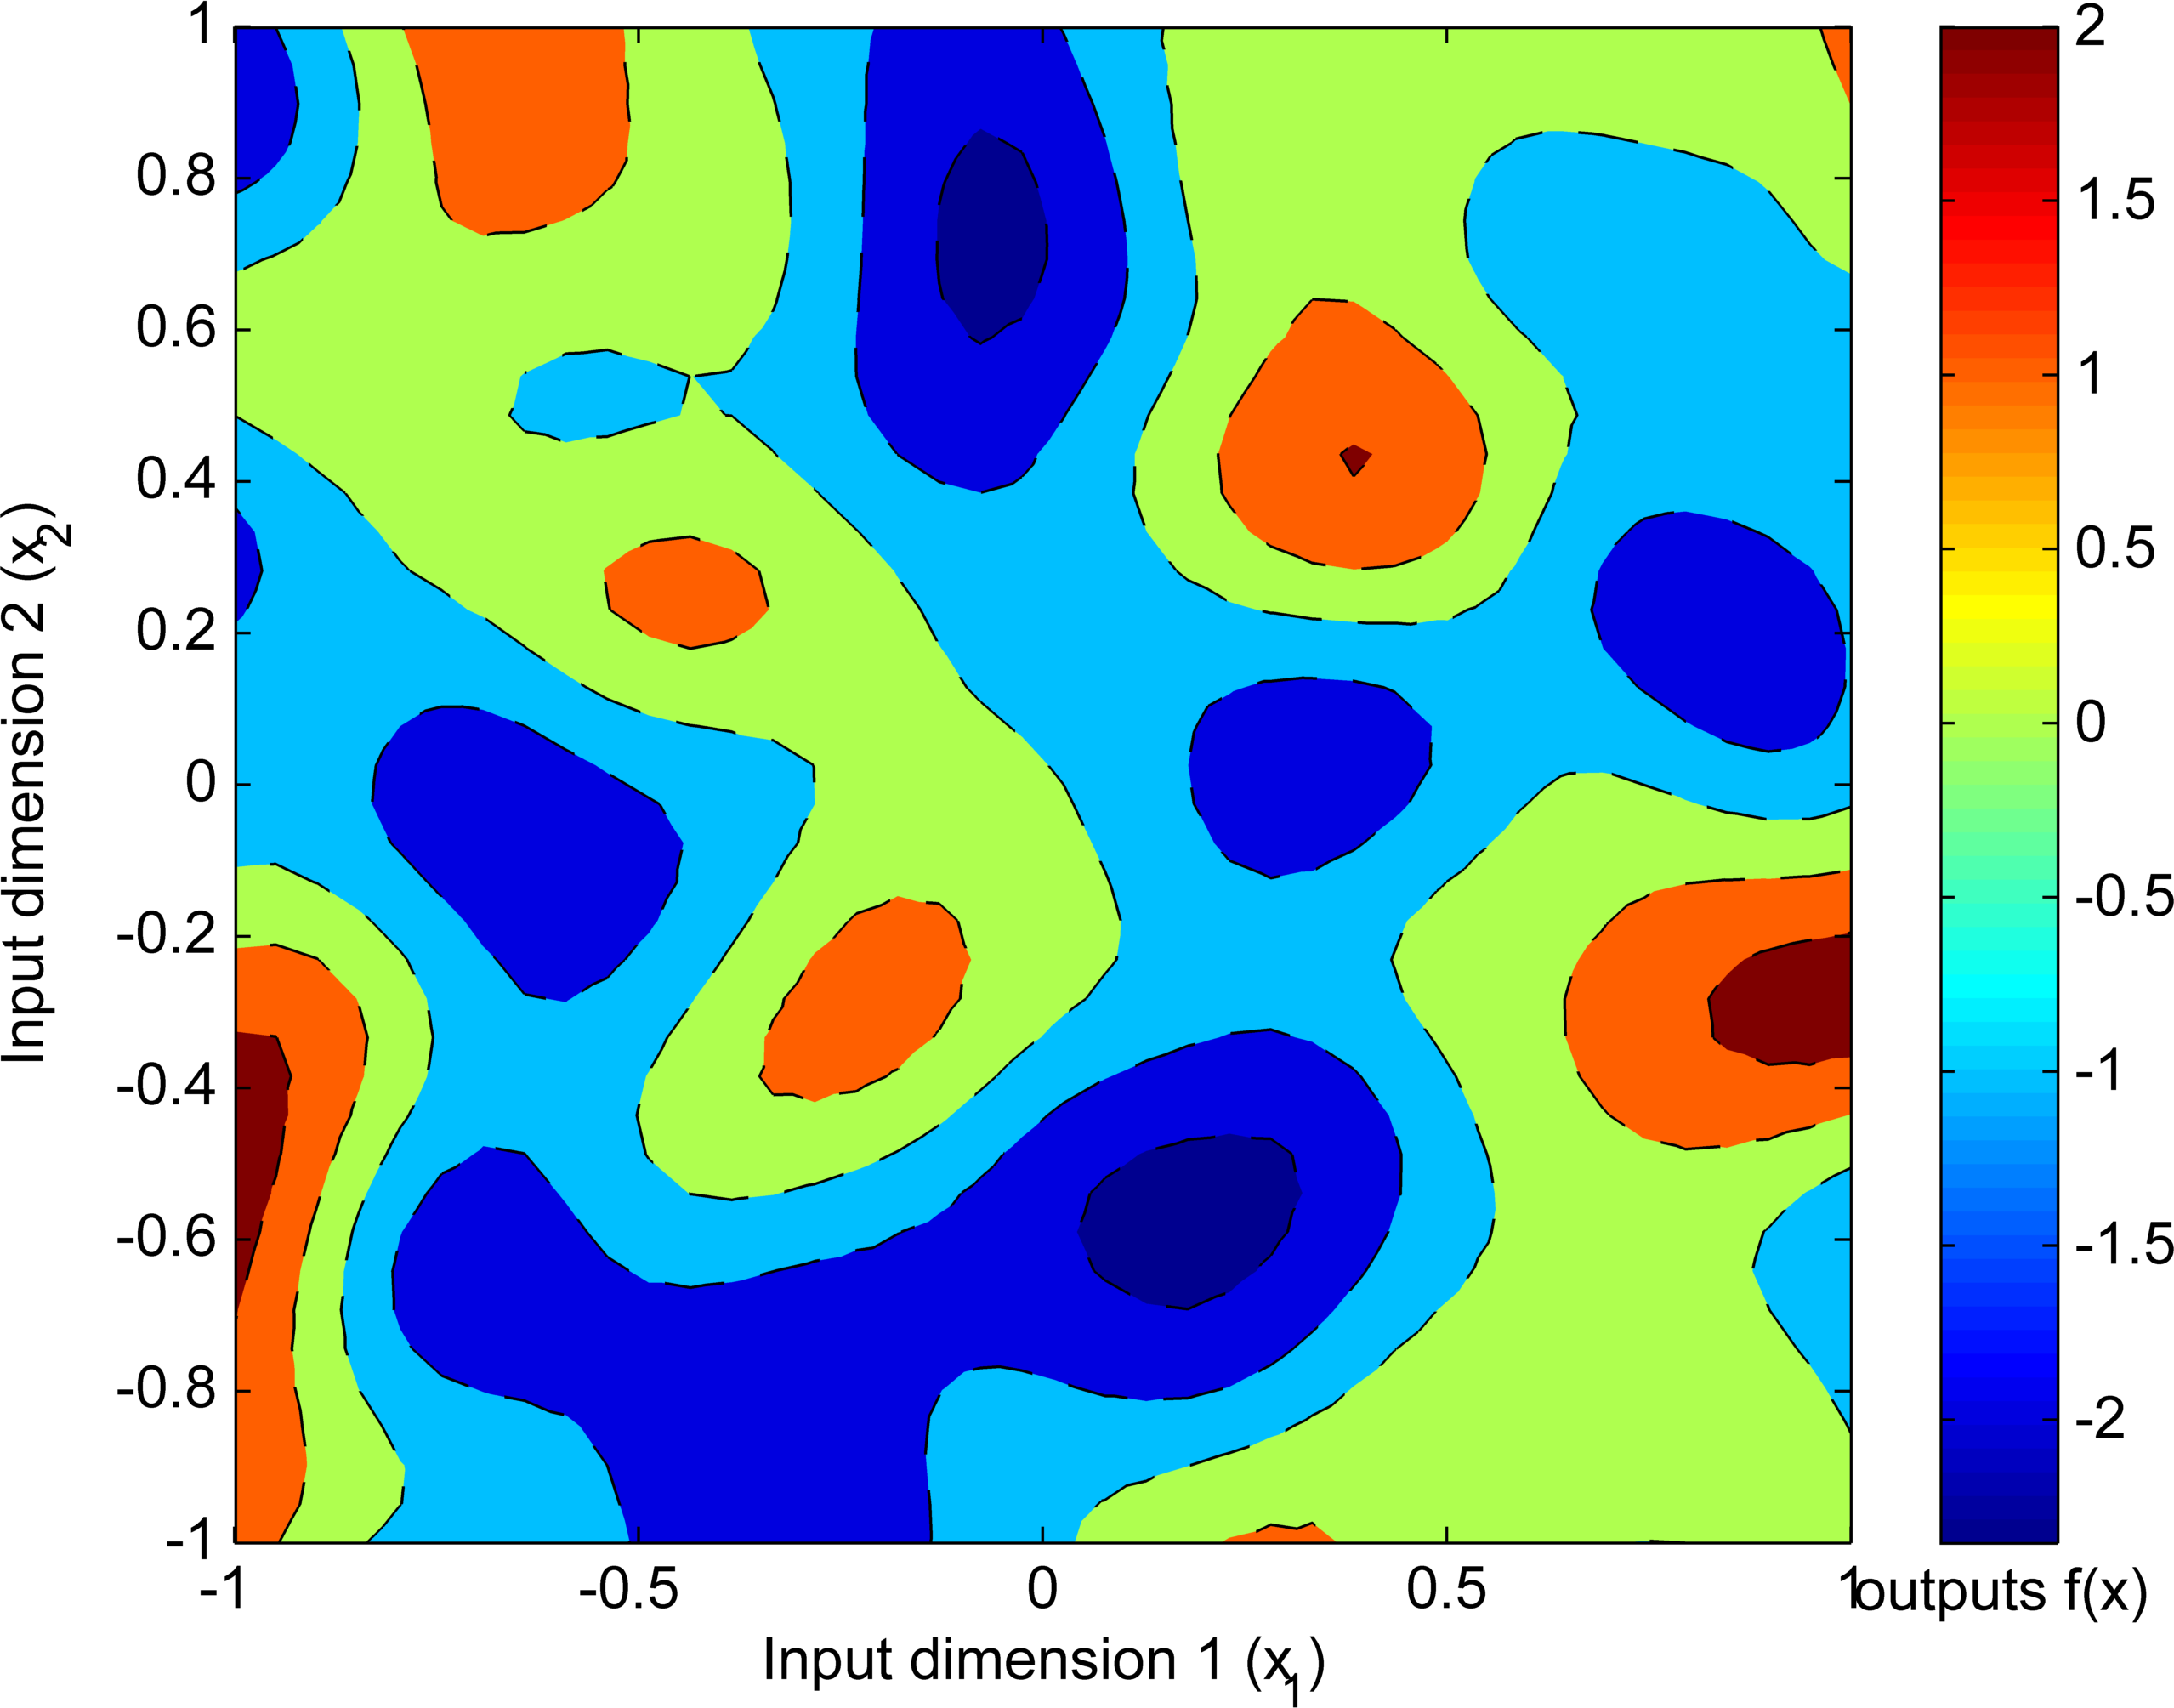
\includegraphics[width=0.45\textwidth]
        {images/part2/drawsProdMultiDimensional}
        \label{subFigdrawsProdMultiDimensional}
  }\quad
\subfigure[{Random draw from a 2 dimensional prior obtained after \textbf{adding} two SE kernels. The hyper-parameters of both the SE kernels are $\theta_{amplitude}=1$ and $\theta_{lengthscale}=1$}]
  {
        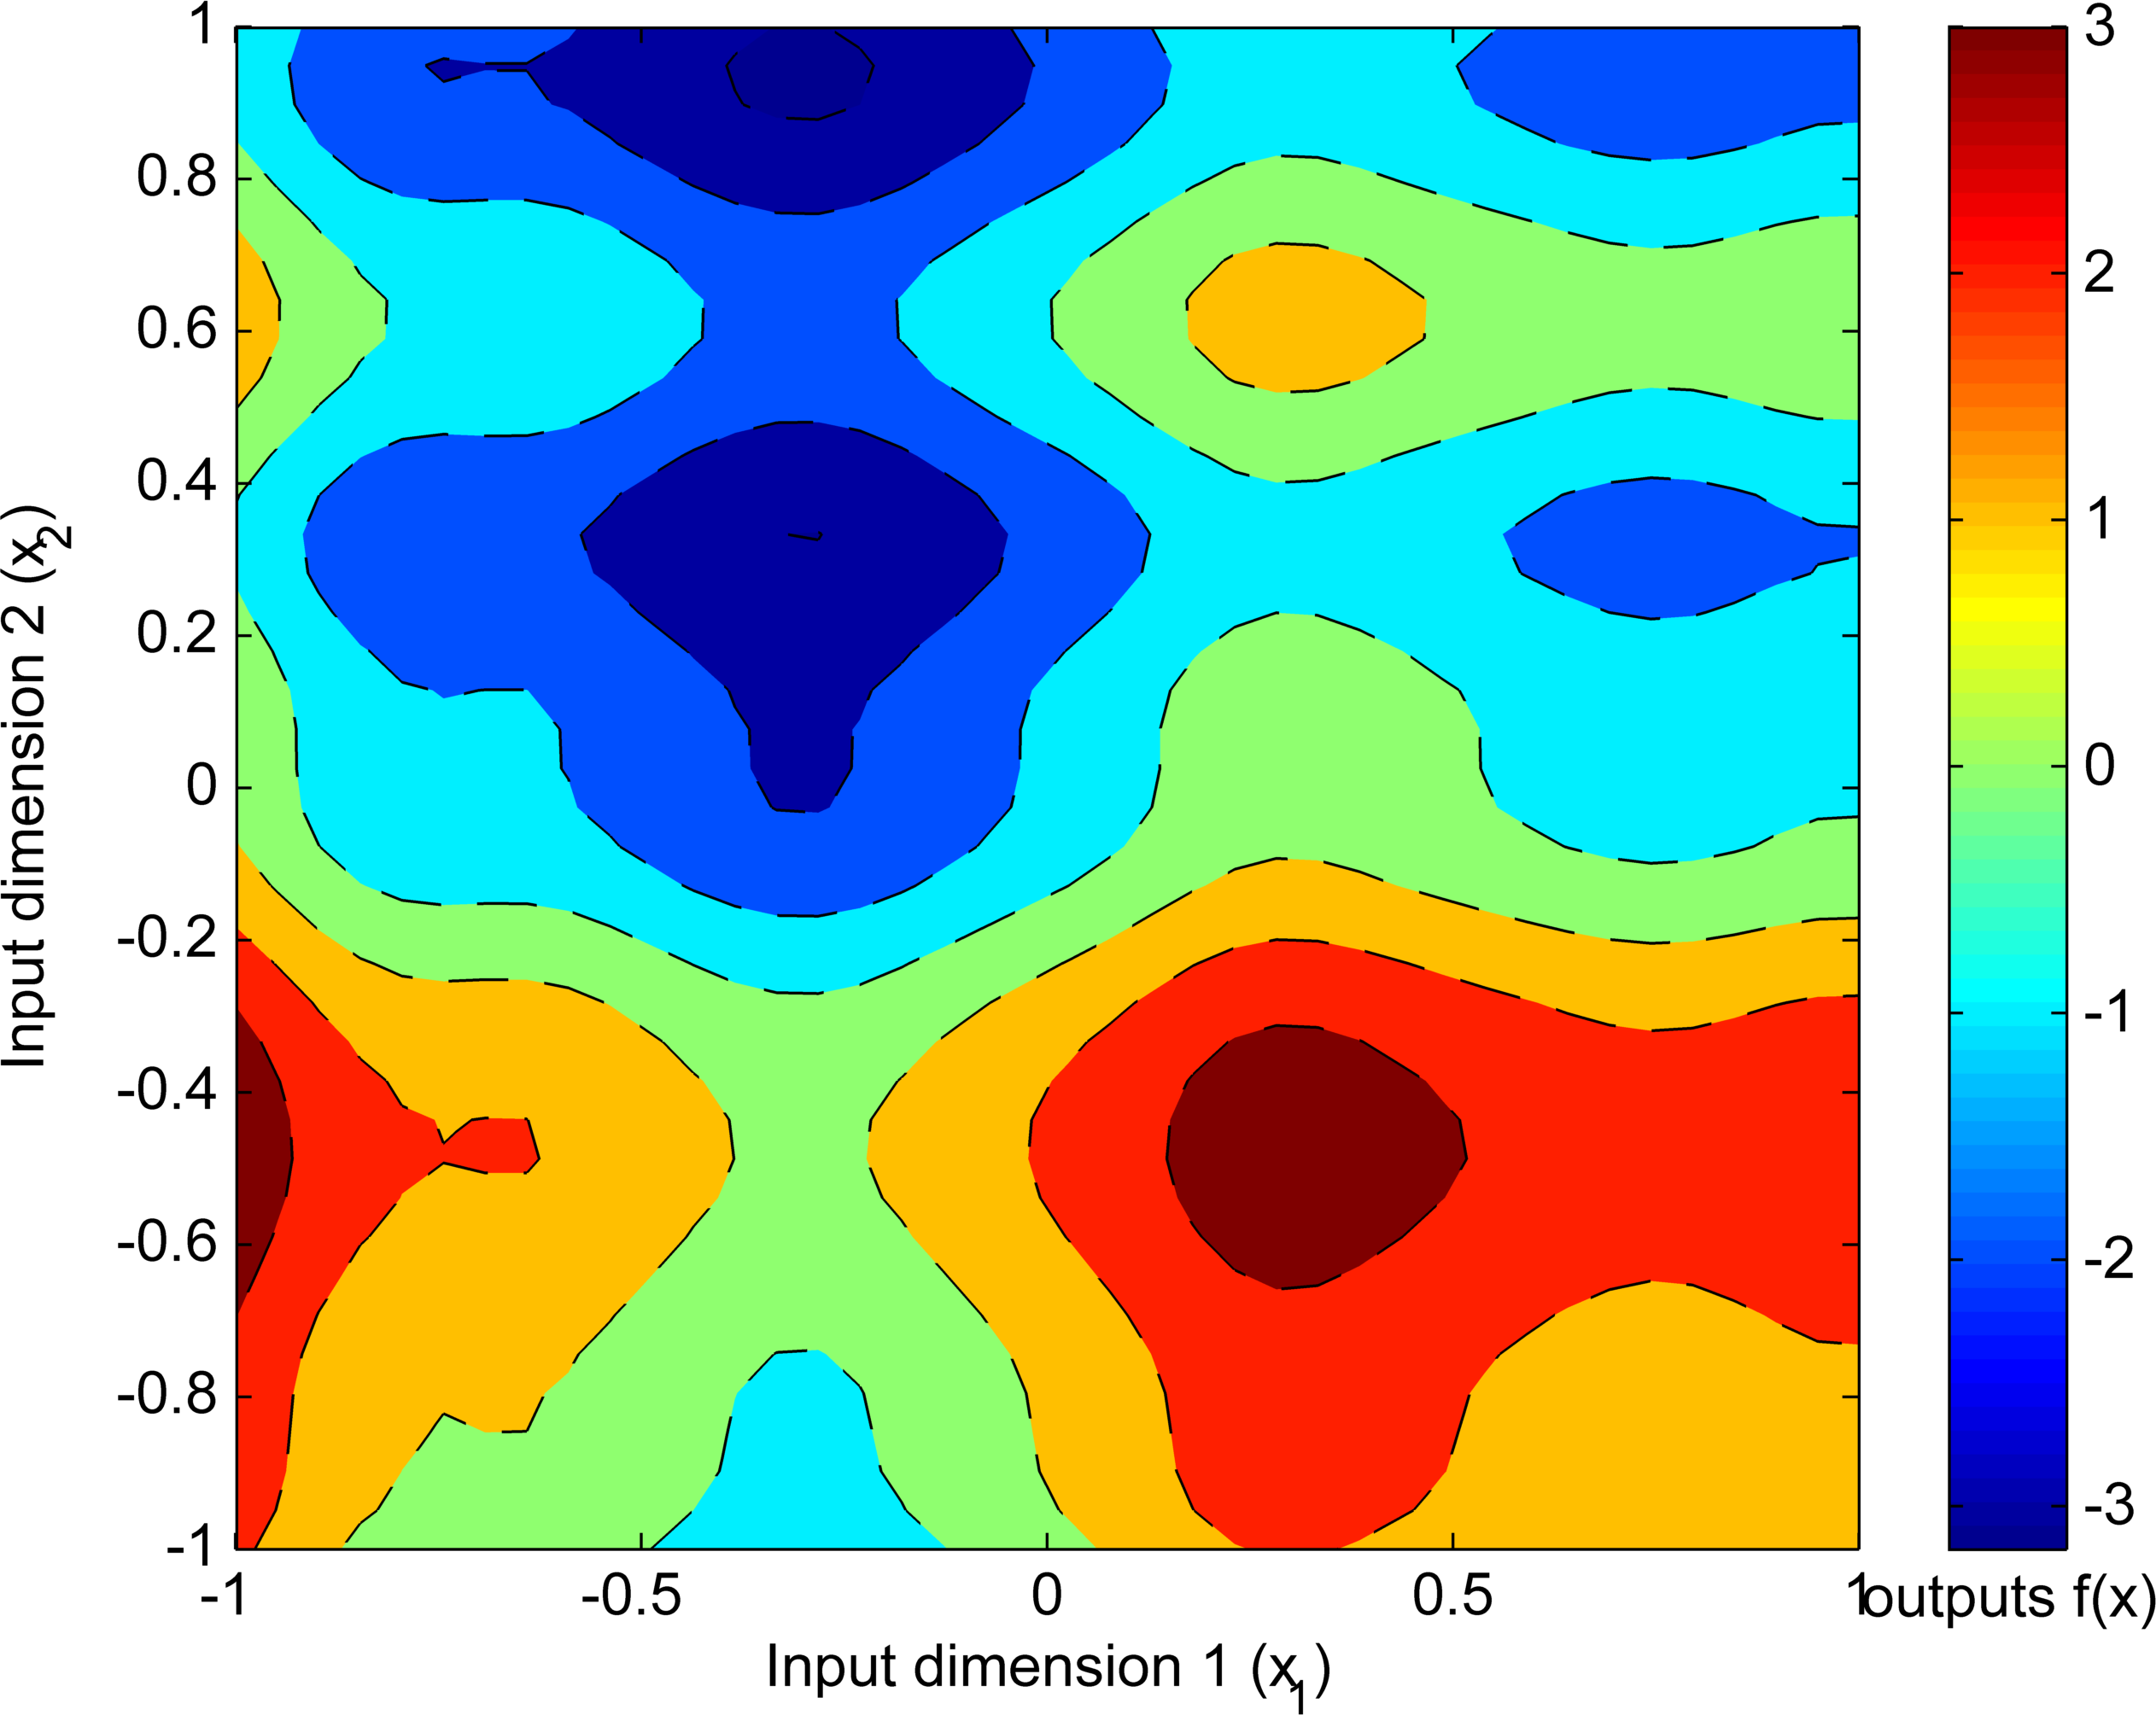
\includegraphics[width=0.45\textwidth]
        {images/part2/drawsSumMultiDimensional}
        \label{subFigdrawsSumMultiDimensional}
  }\quad
       \caption{Random draw from a 2 dimensional prior.}
       \label{figPrior2dimensional}
\end{figure}


Mat\'ern kernels have been found to have superior performance when compared to SE kernels on data-sets with high-dimensions \cite{le2013fastfood}. It is argued that the Mat\'ern kernel accounts for the concentration of measure effect in higher-dimensions. Since SE kernel is inverse Fourier of Gaussian density, high-dimensional samples of an SE kernel will be constrained to surface of the $D_{inputs}$-dimensional ellipse. This problem is less severe for a heavy tailed t-distribution power spectrum of Mat\'ern kernel \cite{wilson2014thesis}. 

\subsection{Sensitivity analysis}
\cite{duvenaud2011additive, durrande2013anova, chastaing2015anova} define a class of additive kernels which are formed upon adding several low-dimensional interactions. Equation \ref{eqANOVAdecomposition} is the basic form of covariance function which can be used to perform sensitivity analysis.

\begin{align}
k(\VEC{x_{1}}, \VEC{x_{2}}) & = (\theta)^2 \prod_{i=1}^{D_{inputs}} \left(1 + k^{i}(x_{1}^{i}, x_{2}^{i})\right) \label{eqANOVAdecomposition} 
\end{align}

The above kernel will include all the possible interactions across dimensions. For example for a 3-dimensional input space, the above kernel will include all the first order terms (equation \ref{eqANOVAfirstOrder}), all the second order terms (equation \ref{eqANOVAsecondOrder}), and the third order term (equation \ref{eqANOVAthirdOrder}).

\begin{align}
k_{first-order}(\VEC{x_{1}}, \VEC{x_{2}}) =  & k^{1}(x_{1}^{1}, x_{2}^{1}) + k^{2}(x_{1}^{2}, x_{2}^{2}) + k^{3}(x_{1}^{3}, x_{2}^{3})\label{eqANOVAfirstOrder} \\
k_{second-order}(\VEC{x_{1}}, \VEC{x_{2}})  = & k^{1}(x_{1}^{1}, x_{2}^{1}) \times k^{2}(x_{1}^{2}, x_{2}^{2}) + k^{2}(x_{1}^{2}, x_{2}^{2}) \times k^{3}(x_{1}^{3}, x_{2}^{3}) \\ & 
+  k^{3}(x_{1}^{3}, x_{2}^{3}) \times k^{1}(x_{1}^{1}, x_{2}^{1}) \label{eqANOVAsecondOrder} \\
k_{third-order}(\VEC{x_{1}}, \VEC{x_{2}}) = & k^{1}(x_{1}^{1}, x_{2}^{1}) \times k^{2}(x_{1}^{2}, x_{2}^{2}) \times k^{3}(x_{1}^{3}, x_{2}^{3})\label{eqANOVAthirdOrder} \\
\end{align}


These kinds of kernels can be used to analyze the sensitivity of interactions between various dimensions (also called as ANalysis Of VAriance, ANOVA). 

\subsection{Low dimensional structure}
We can also encode a low dimensional structure into family of functions by specifying the kernel as $k_{low} = k(\VEC{x_{1}}\myMatrix{H}, \VEC{x_{2}}\myMatrix{H})$ (equation \ref{eqCh5ComposedCovariances}), here $\myMatrix{H}$ is a low rank matrix. 

\begin{align}\label{eq:SELowDimensional}
k_{low}(\VEC{d}, \VEC{\theta}) = (\theta_{amplitude})^2  exp\left [  -\frac{1}{2} \VEC{d} \myMatrix{\Sigma} \VEC{d}^T \right ] 
\end{align}

Here, $\myMatrix{\Sigma}$ is $\myMatrix{H}\myMatrix{H}^T/(\theta_{lengthscale}^2)$ which encodes the low dimensional structure. Figure \ref{subFigdrawsLowMultiDimensional} is obtained after encoding a low-dimensional into SE kernels, the hyper-parameters of the SE kernel are $\theta_{amplitude}=1$ and $\theta_{lengthscale}=0.2$ while $\myMatrix{\Sigma} = \bigl( \begin{smallmatrix} 1 & 0\\ -1 & 0\end{smallmatrix}\bigr)$. 

\begin{figure}[!ht]
  \centering
   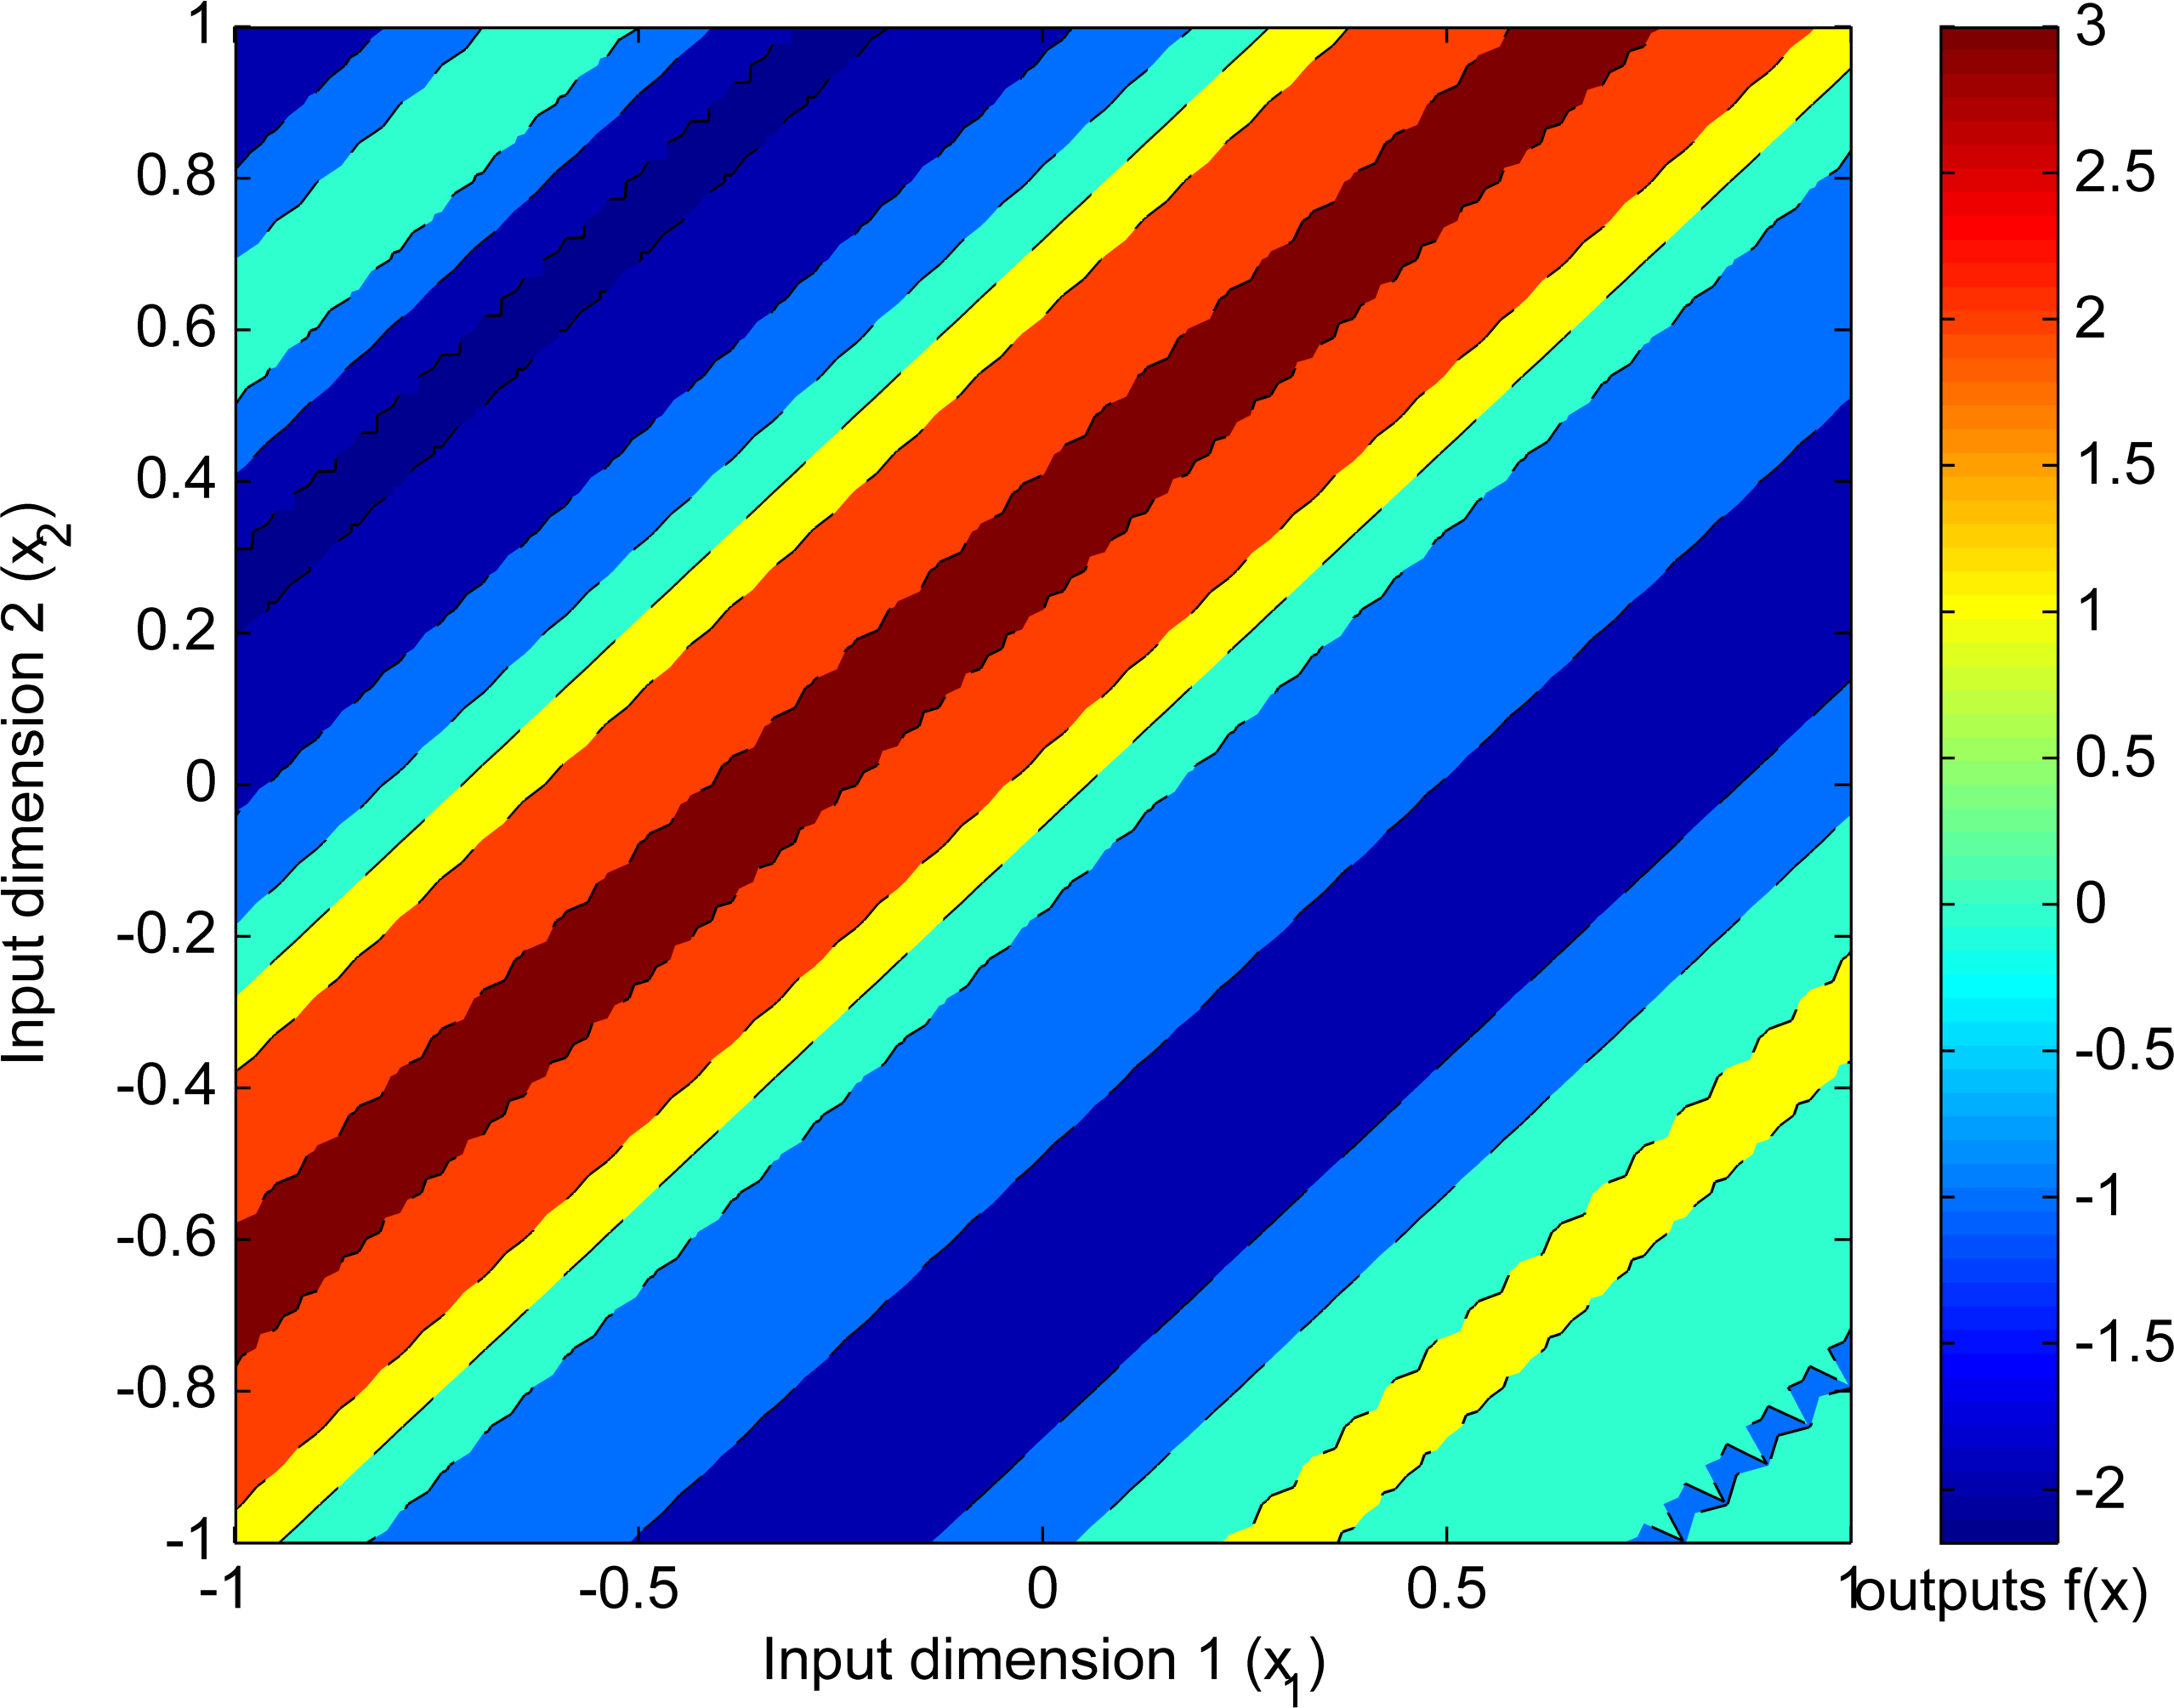
\includegraphics[width=0.45\textwidth]
        {images/part2/drawsLowMultiDimensional}
        \label{subFigdrawsLowMultiDimensional}
  \caption{Random draw from a 2 dimensional prior which encodes a \textbf{low-dimensional} structure. The hyper-parameters of the kernel are $\theta_{amplitude}=1$ and $\theta_{lengthscale}=1$}
\end{figure}

When $\myMatrix{\Sigma}$ is a diagonal matrix we get an ARD kernel

\begin{equation}
\begin{aligned}
k(\VEC{d}, \VEC{\theta}) & = (\theta_{amplitude})^2  exp\left [  -\frac{1}{2} \VEC{d} \myMatrix{\Sigma} \VEC{d}^T \right ] = 
(\theta_{amplitude})^2  exp\left [ \sum_{i=1}^{D_{inputs}} -\frac{(d^{i})^2}{2(\theta_{lengthScale}^{i})^2} \right ] \\
& = (\theta_{amplitude})^2 \prod_{i=1}^{D_{inputs}}  exp\left [ -\frac{(d^{i})^2}{2(\theta_{lengthScale}^{i})^2} \right ]
\end{aligned}
\end{equation}

\marginnote{\textsl{KPLS}}[1cm]
When the number of dimension increases significantly, the number of hyper-parameters also increases this makes the optimization of marginal likelihood inefficient. \cite{bouhlel2016improved} first reduce the dimensionality of the data-set and then perform interpolation thereby circumventing the problem of higher dimensions. \cite{garnett2013active, tripathy2016gaussian} use this covariance to reduce the dimensionality of input domain.

In the current section we have seen how to build covariance functions for multi-dimensional inputs. We now apply multi-dimensional kernels to build a surrogate model for Aerodynamic pressures. We validate our method on 2 test cases: the first in subsonic regime on a Flap Track Fairing (FTF) and the second in transonic regime on NASA's Common Research Model (CRM) Wing. The reader can also note that the results of these experiments were used during a recent Airbus Flight test campaign.

\subsection{Application: Interpolation of aerodynamic pressures}\label{subecInterpolationOfAerodynamicPressures}
Accurate prediction of aerodynamic pressures at a flight configuration is computationally expensive. Hence, it becomes advantageous to use surrogate models as approximations of high-fidelity aerodynamic models. A popular method of surrogate modelling in the aerodynamics community is by interpolating Reduced Order Models (ROM). A set of aerodynamic pressure snapshots is generated by performing CFD simulations for different aerodynamic parameters (eg. angle of attack $\alpha$, Mach). Then orthogonal basis vectors are found in the parameter space for the set of pressures snapshots. Generally, Proper Orthogonal Decomposition (POD) \cite{tan2003proper, rosenbaum2013efficient, braconnier2011towards} (also called as Principal Component Analysis (PCA) or Singular Value Decomposition (SVD)) is used to find the linear subspace. Finally, the reduced models are interpolated at the desired point in the parameter-space \cite{beckert2001multivariate, barrault2004empirical}. 

\marginnote{\textsl{Pressure snapshot}}[1cm]
Let us first start by defining a pressure snapshot. There exists a \(3\) dimensional spatial vector \(\VEC{\omega_{i}} \in  \mathbb{R}^{3}\) such that \(\VEC{\omega_{i}} = \{(\omega_{i}^{1}, \omega_{i}^{2}, \omega_{i}^{3})\}\). Here, \(i \in [1,N_{nodes}] \) are the spatial coordinates of the \(i^{th}\) pressure node in a CFD mesh containing \(N_{nodes}\) pressure nodes. Similarly there exists a \(D\) dimensional parameter vector \(\VEC{d_{j}} \in  \mathbb{R}^{D}\), for \(\VEC{d_{j}} = \{(d_{j}^{1}, d_{j}^{2}, \ldots ,d_{j}^{D})\}\). Here,   \(j \in [1,N_{experiment}] \) correspond to the \(j^{th}\) parameter set, while $D$ corresponds to the number of parameters. The parameters can be any parameters which are desired to be interpolated, some common examples include Mach, Angle of Attack for steady aerodynamics and time or frequency for unsteady aerodynamics. We will only concentrate on interpolating steady aerodynamics in this section.

The pressure measured on the \(i^{th}\) pressure node for the \(j^{th}\) parameter set will be denoted as \(p_{j}(\VEC{\omega_{i}})\) defined by equation \ref{eq:pijSnapshot}. We next define the matrix \(\myMatrix{\Omega} = \{\VEC{\omega_{1}}; \VEC{\omega_{2}}; \ldots ; \VEC{\omega_{N_{nodes}}}\}\) for \(\myMatrix{\Omega} \in \mathbb{R}^{N_{nodes} \times 3}\) containing the full spatial information of the aerodynamic mesh. Finally, the pressure snapshot for the CFD/experiment run \(j\) will be denoted as \(\VEC{P_{j}(\Omega)} = \{p_{j}(\VEC{\omega_{1}}); p_{j}(\VEC{\omega_{2}}); \ldots ; p_{j}(\VEC{\omega_{N_{nodes}}})\}\) for \(\VEC{P_{j}(\Omega)} \in \mathbb{R}^{N_{nodes}}\) defined by the equation \ref{eq:pressurefield}.

\begin{equation} \label{eq:pijSnapshot}
p_{j}(\VEC{\omega_{i}}) = f_{pressure}(\VEC{\omega_{i}}, \VEC{d_{j}})
\end{equation} 
\begin{equation}\label{eq:pressurefield}
\VEC{P_{j}(\Omega)} = f_{pressure}(\myMatrix{\Omega}, \VEC{d_{j}})
\end{equation} 

Here, $f_{pressure}$ symbolizes the aerodynamic process which when applied to a spatial location ($\VEC{\omega}$) and an aerodynamic parameter ($\VEC{d}$) gives us the pressures, we eventually wish to approximate this process ($f_{pressure}$). The POD methodology decomposes the set of pressure snapshots ($\VEC{P_{j}(\Omega)}$) into their eigen vectors ($\VEC{\phi^{l}(\Omega)}$) and participation factors ($a^{l}(\VEC{d_{j}})$). To reconstruct the pressure snapshot at a new point $\VEC{d_{new}}$, the participation factors are interpolated and then linearly combined to give the new pressure snapshot (equation \ref{eq:interpPODEquation}). For more details please refer to appendix \ref{appPODI}
\marginnote{\textsl{POD}}[-1cm]

\begin{equation}\label{eq:interpPODEquation}
\VEC{P_{new}(\Omega)} = \sum_{l=1}^{p}a^{l}(\VEC{d_{new}}) \VEC{\phi}^l(\myMatrix{\Omega})
\end{equation}

\begin{mdframed}[hidealllines=true,backgroundcolor=blue!20]
\marginnote{\textsl{Contribution}}[1cm]
Due to the assumption of linear subspace, interpolation through ROM is highly efficient both in terms of cost and performance in the subsonic regime \cite{verveld2016reduced}. Unfortunately in the transonic regime, the shock creates a highly non-linear, almost discontinuous pressure distribution and the assumption of linear subspace does not hold \cite{li2016performance}. Although the performance of ROM interpolators can be improved with larger number of samples \cite{franz2014interpolation, forrester2008engineering}, we propose to improve the accuracy of prediction using the Distributed GPs regression for the same number of samples.  

We interpolate the pressure $p_{j}(\omega_{i})$ by simply multiplying the kernels across dimensions (equation \ref{eqSubsonicPressureGP}). To interpolate in subsonic regime we multiply Mat\'ern $\nu=5/2$ across dimensions, a Mat\'ern kernel is chosen since it does not suffer from concentration of measure effect in higher dimensions. We are not interested in linearly separating the effects of individual dimensions, hence a simple multiplicative kernel will suffice for this problem. 

\begin{equation}\label{eqSubsonicPressureGP}
\Pr[p_{j}(\omega_{i})] = GP \left( 0, k(x_{1}, x_{2}) = \prod_{i=1}^{D_{inputs}} k_{Mat (\nu =5/2)}(x_{1}^{i}, x_{2}^{i}) \right)
\end{equation}

The transonic regime often contains a shock on the surface of the wing. This shock almost creates a discontinuity in the pressure field. We know from section \ref{subSecCh4NNkernel} that Neural Network kernels can represent these type of almost discontinuous functions in its hypothesis space. Hence to interpolate in transonic regime we use the Neural Network kernel in the dimension of shock. For example, if we know that the shock appears on the chord-wise direction, then we can represent the pressure as equation \ref{eqTransonicPressureGP}.

\begin{equation}\label{eqTransonicPressureGP}
\Pr[p_{j}(\VEC{\omega_{i}})] = GP \left( 0, k(\VEC{x_{1}}, \VEC{x_{2}}) = k_{NN}(x_{1}^{chord}, x_{2}^{chord}) \times \prod_{i=1}^{D_{inputs-1}} k_{Mat (\nu =5/2)}(x_{1}^{i}, x_{2}^{i}) \right)
\end{equation}

Here, $x_i^{chord}$ represents the chord wise dimension of the $i^{th}$ input, while $k_{NN}$ and $k_{Mat \nu =5/2}$ represent the Neural Network and Mat\'ern ($\nu=5/2$) kernels respectively.
\end{mdframed}

We now test the performance of Distributed GPs and POD+I on two sets of numerical experiments. Firstly, we test the accuracy on a detailed Flap Track Fairing (FTF) design \cite{bosco2016nonlinear} in subsonic regime (section \ref{subSec:elsAResults}) based on RANS simulation from the elsA solver \cite{cambier2008status}. Finally, we compare the accuracy on CRM wing in the transonic regime using the elsA solver and a k-Omega-SST turbulence model \cite{vassberg2014summary}. elsA\textsuperscript{\textregistered} \cite{cambier2008status} is a CFD simulation platform that allows representation of both internal and external aerodynamics from the low subsonic to the high supersonic flow regime.  

\subsubsection{Interpolation in subsonic regime}\label{subSec:elsAResults}
\marginnote{\textsl{FTF}}[1cm]
A FTF is situated below the wing and is used to deploy flaps for landing and take-off configurations. A FTF experiences heavy dynamic excitation due to the exhaust coming from engine. The dynamic nature makes the design of FTF a challenging task, where each simulation can last for 2 days. If we can effectively interpolate pressure snapshots then a 2 day dynamic simulation can be reduced to a few hours. 

Interpolation of FTF pressure snapshots has been earlier studied using POD methodology \cite{bosco2016nonlinear}. In this section we use this data-set to validate the interpolation capabilities of a Distributed GPs algorithm. 


\begin{figure*}[!ht]
  \centering
  \subfigure[FTF Pressure snapshot]
  {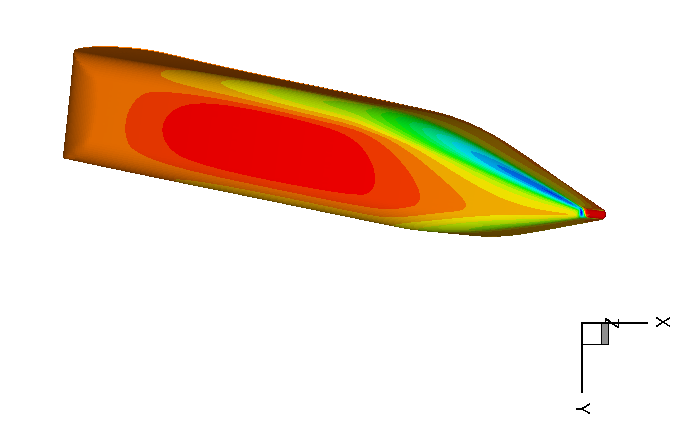
\includegraphics[height=0.15\textheight]{images/part2/RANS_m6}\label{fig:ftf_snapshot}}\quad
  \subfigure[FTF parameters $\VEC{d_i} = (\theta_i, \alpha_i)$]
  {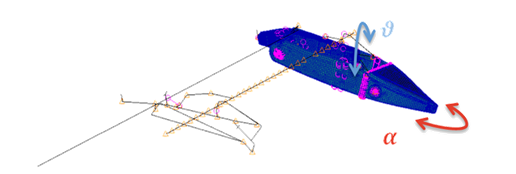
\includegraphics[height=0.15\textheight]{images/part2/ftf_dof}\label{fig:ftf_dof}}\quad
      \caption{Details of the FTF}
\end{figure*}

The FTF parameters chosen for this analysis are $\theta$, the rotation around the longitudinal axis of the FTF, and $\alpha$, the rotation around the {\it spigot} axis, main connection between the track and the wing structure figure \ref{fig:ftf_dof}. The surface mesh of the CFD skin contains almost 36 thousand nodes (more precisely $N_{nodes} = 36802$). We run the simulation for 9 different values of $\alpha$ and 9 different values of $\theta$ ($N_{experiment} = 9\times9 = 81$). In this particular case Reynolds Averaged  Navier-Stokes (RANS), equations are used with Spalart-Allmaras turbulence model to simulate the flow around the FTF. Figure \ref{fig:ftf_snapshot} shows one particular pressure snapshot. 
\marginnote{\textsl{$\VEC{d_i} = (\theta_i, \alpha_i)$}}[-1cm]

\marginnote{\textsl{LOO-CV}}[1cm]
We use the Leave One Out (LOO) Cross Validation method to quantify the performance of the two methodologies. $[\alpha, \theta]$ pairs are removed one by one from the database to create a new training set. The new training set is used to perform interpolation according to POD+I and Distributed GPs. Pressure snapshot is reconstructed for the missing $[\alpha, \theta]$ pairs. The methods are finally compared by evaluating the Root Mean Square Error (RMSE) and time of prediction for each pair case. 

\marginnote{\textsl{Distributed GPs }}[1cm]
While performing Distributed GPs regression, we learn a model between the input vector $\VEC{x_{ij}} = [\omega_{i}^{1}, \omega_{i}^{2}, \omega_{i}^{3}, \alpha_j, \theta_j]$ and the pressures ($y_{ij} = p_{ij}$). We build a multi-dimensional kernel by multiplying 5 Mat\'ern kernels, different length-scale for each dimension. As discussed earlier we propose to use Mat\'ern kernel since the SE kernel has a very restrictive hypothesis space for high-dimensional regression.  Effectively we are learning a GP model for $N = 36802\times80 = 2.9$ million data-points, there are 1000 points in each expert. 

\begin{figure*}[!ht]
  \centering
  \subfigure[{Box plots of normalized RMSE for the two different model types. POD has a RMSE of $0.48\pm0.27$ whereas Distributed GPs has a RMSE of $0.37\pm0.1$. The mean Distributed GPs prediction is $20\%$ better than POD. Outliers are extrapolation cases }]
  {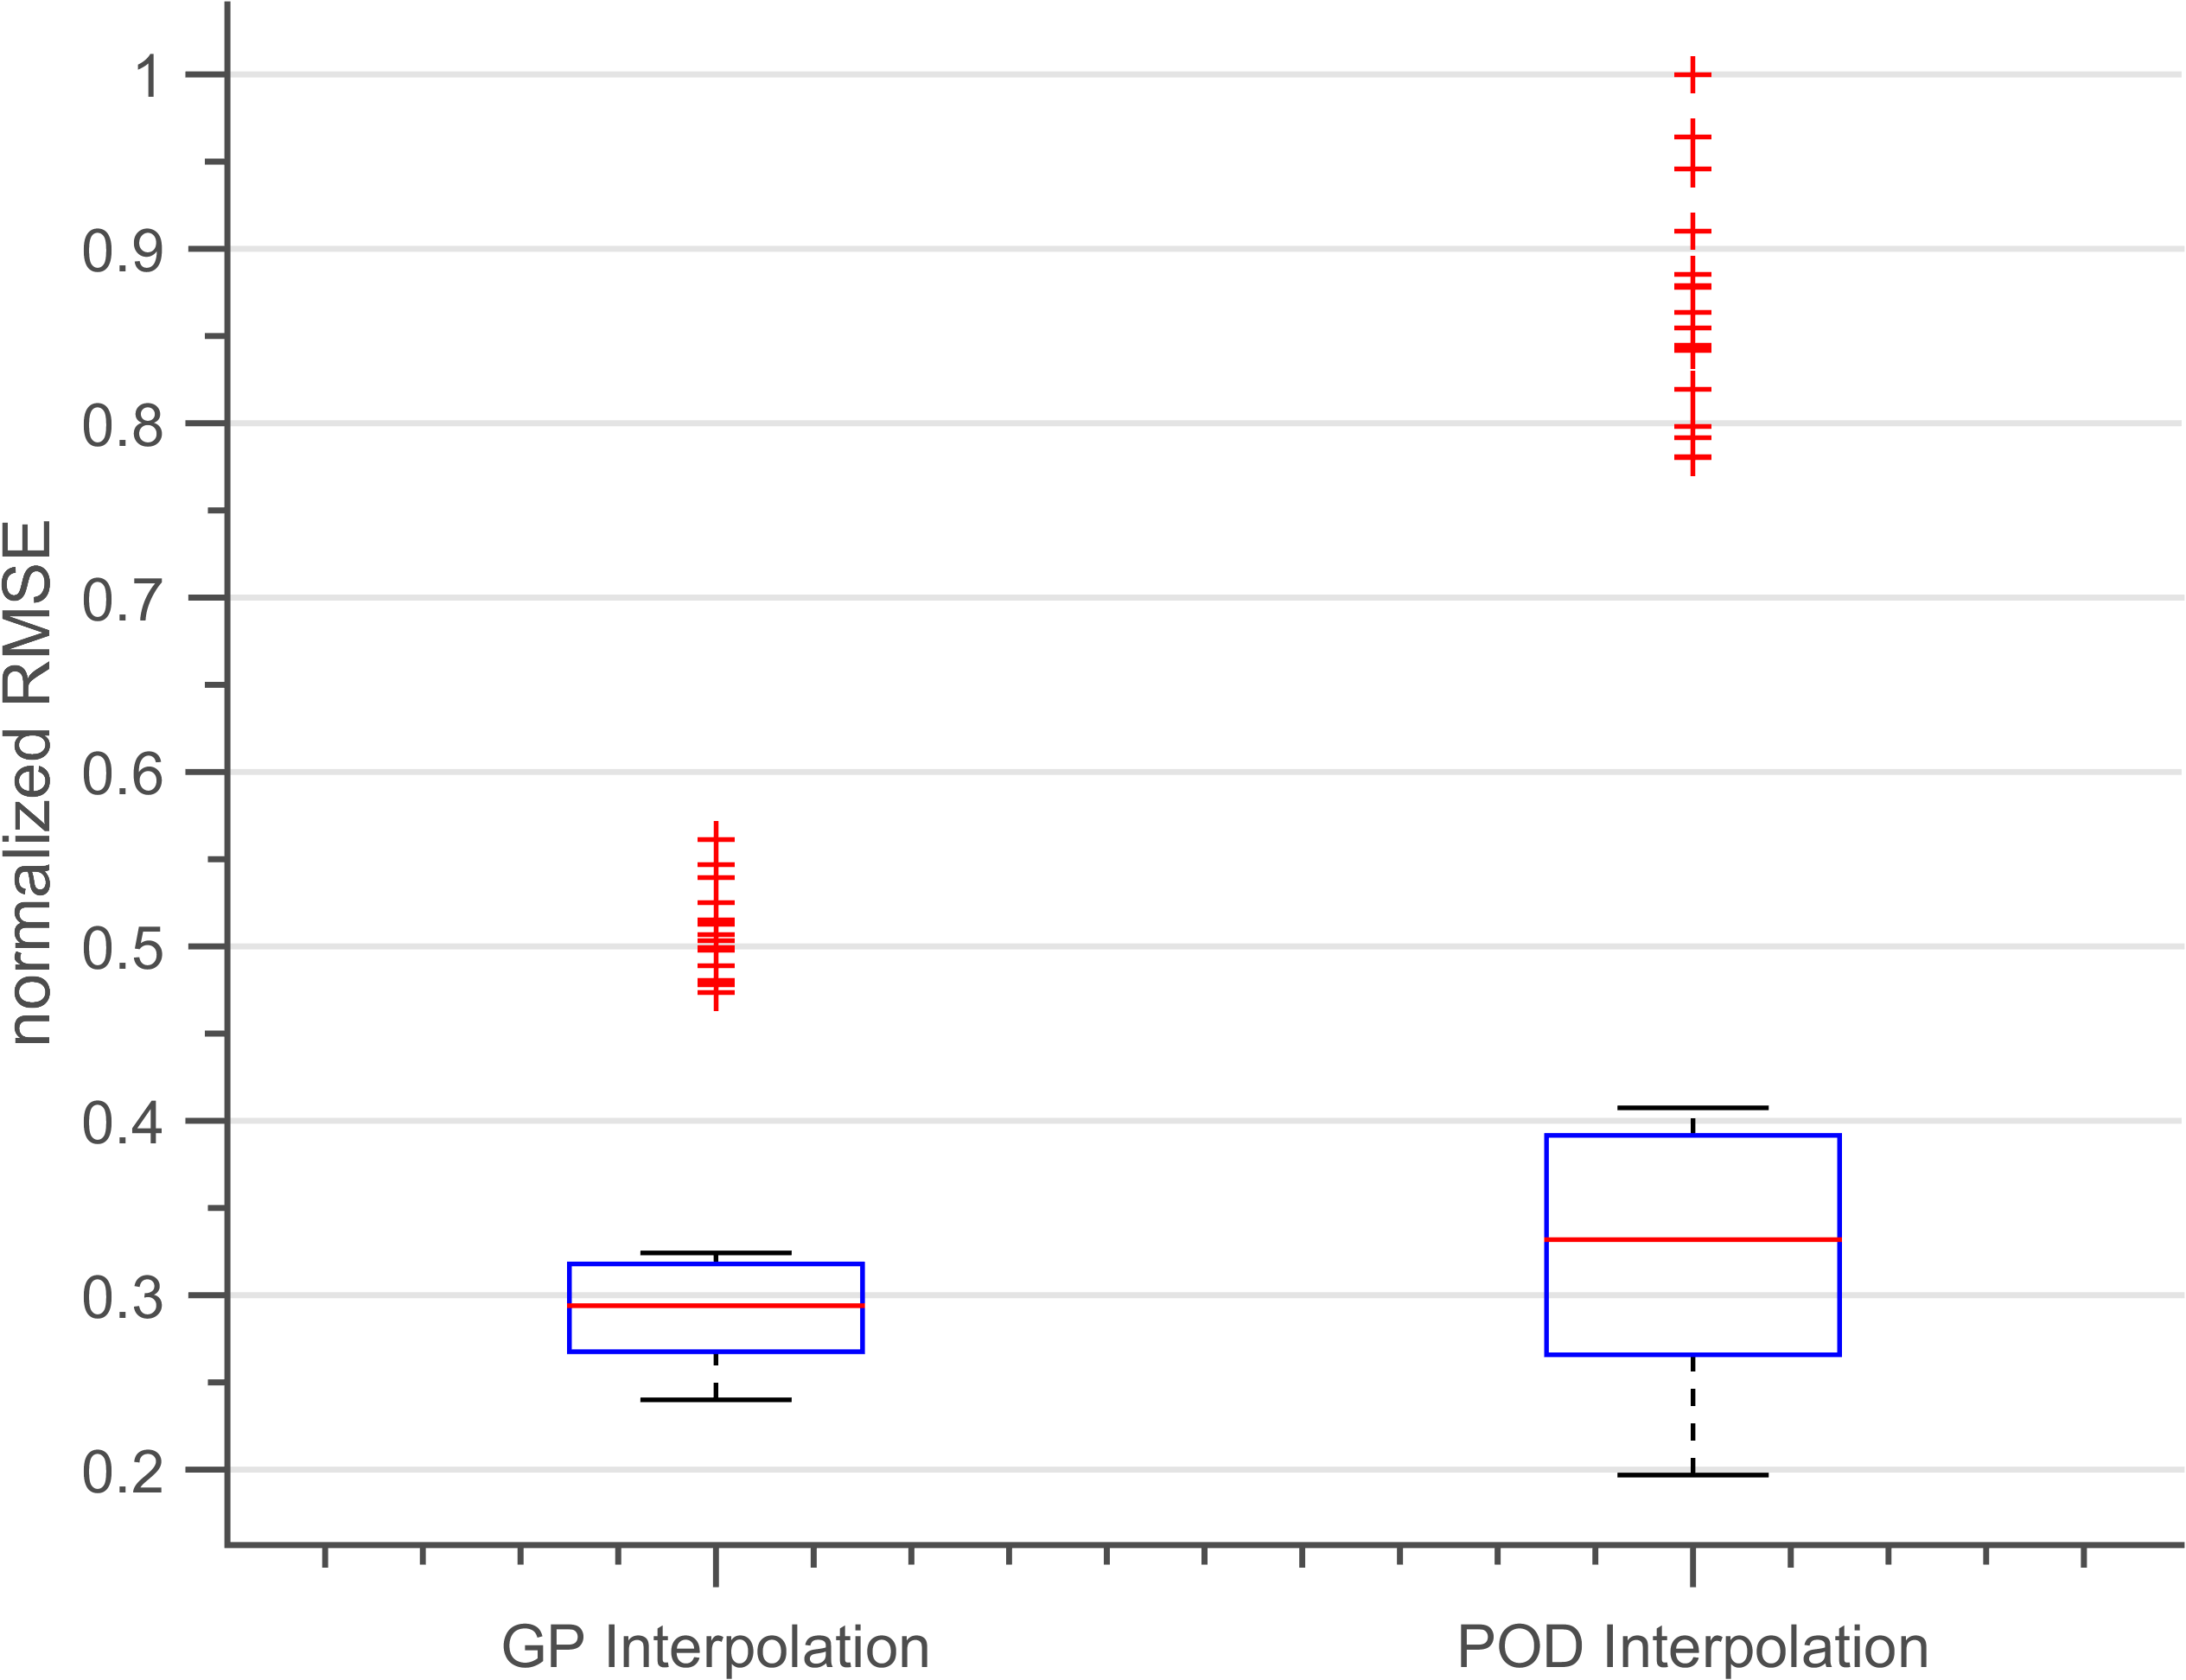
\includegraphics[width=0.45\textwidth]{images/part2/rmse_AST}\label{subfig:RMSECFD}}\quad
    \subfigure[{Time taken to perform prediction for the two different model types. 
    POD takes $2.35s\pm0.11s$ whereas Distributed GPs takes $37.84s\pm4.35s$ to perform the interpolation. The average POD method is 19 times faster than Distributed GPs.}]
    {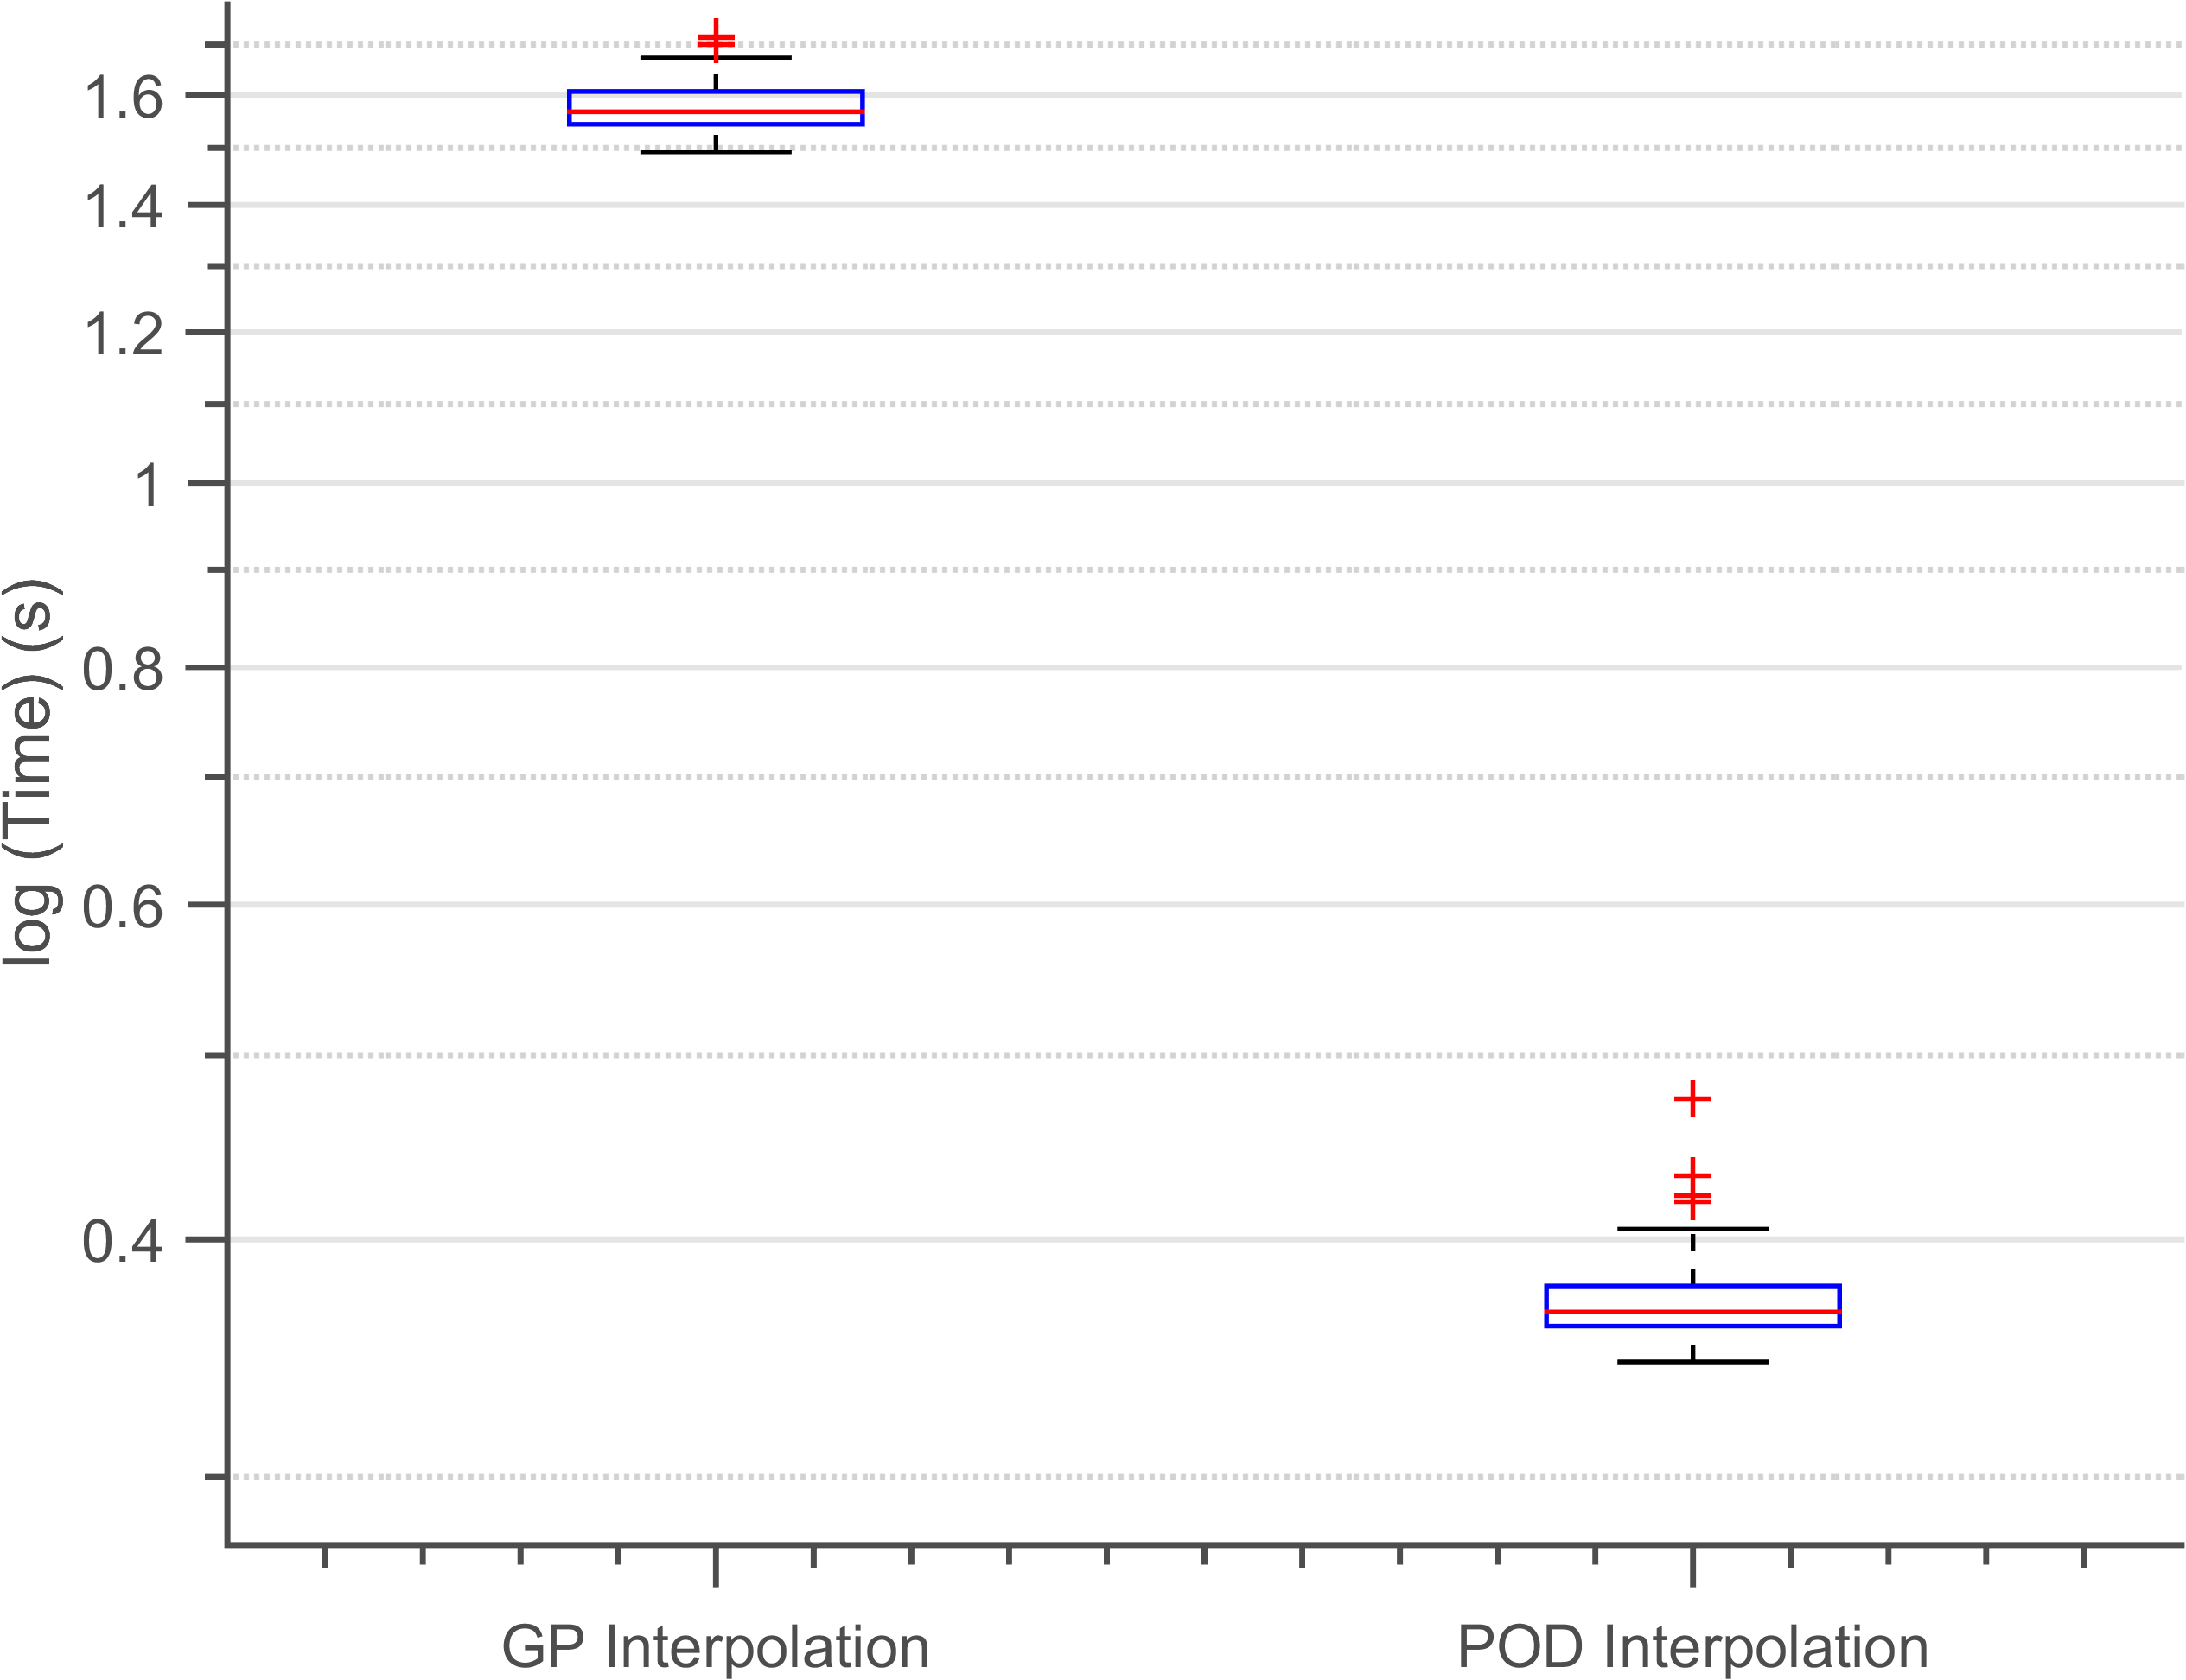
\includegraphics[width=0.45\textwidth]{images/part2/time_AST}\label{subfig:timeCFD}}
  \caption{Results for elsA interpolation}
  \label{fig:FTF_CFDresults}
\end{figure*}

Figures \ref{subfig:RMSECFD} denote the RMSE estimates for different pairs. For RMSE, the Distributed GPs performs marginally better than POD. The outliers in the box-plots denote cases where the removed pairs are on the edges of the domain. Since the removed pairs are on the edges of the domain, there are no CFD snapshots surrounding these pairs. Hence we are extrapolating during the edge cases. POD has a RMSE of $0.48\pm0.27$ whereas Distributed GPs has a RMSE of $0.37\pm0.1$. The average Distributed GPs prediction is $20\%$ better than POD. Figure \ref{subfig:timeCFD} shows the time taken to perform prediction for the two model types. We are only comparing the time to perform interpolation, time to learn the models will be much longer. POD takes $2.35s\pm0.11s$ whereas Distributed GPs takes $37.84s\pm4.35s$ to perform the interpolation.  
\marginnote{\textsl{Figure \ref{fig:FTF_CFDresults}}}[-1cm]

Although the GP technique can more efficiently capture non-linear behavior we see a relatively low improvement in performance for the amount of time invested. Deciding between the simple and time-tested POD method or costly and accurate Distributed GPs interpolation in the subsonic regime can be a delicate task and mostly depends on the preferences of the final user.

\subsubsection{Interpolating in transonic regime}\label{subSec:resultsCRM}
We now proceed to compare the accuracy of the two methods in transonic regime on the CRM wing model proposed by NASA. Since the introduction of the CRM for the 4th Drag Prediction Workshop \cite{vassberg2014summary}, the CRM has been become a very widely used test case for applied computational aerodynamics. Due to the widespread experience and availability of wind-tunnel test results for the CRM configuration, it is a natural case to benchmark interpolations. 

\marginnote{\textsl{Shocks}}[1cm]
Due to the shape of an airfoil, airflow is accelerated on the upper surface of the wing. This causes shocks to appear on the upper surface of the wing in the transonic regime. Shocks are sudden changes (almost discontinuous) in pressure and are important for estimating the performance of the aircraft \cite{jameson1974iterative, cole2012transonic}. Moreover, an aircraft flies in the transonic regime for 80\% of its journey (cruise). Hence accurate prediction of location and strength of a shock is very important during design. Since POD is a linear subspace reduction method it has difficulties in interpolating a discontinuous shock regime \cite{verveld2016reduced}.

\begin{figure*}[!ht]
  \centering
  \subfigure[{CRM. The four red lines are the four cuts at $y/b = [0.105, 0.37, 0.5, 0.84]$. Here, $y$ denotes the y-distance from aircraft axis and $b$ denotes the span of one wing}.]
  {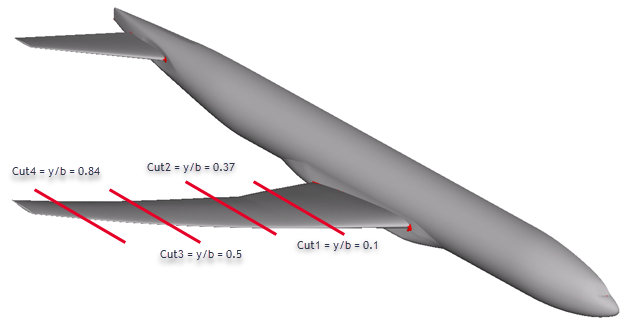
\includegraphics[width=0.45\textwidth]{images/part2/crm_Wing_design}\label{subfig:crmWing}}\quad
    \subfigure[{Pressure snapshot on the CRM for $\alpha = 2$ and $Mach = 0.85$, using elsa solver and $\kappa - \omega$ SST turbulence model. We can observe double shock pattern appearing on the outer sections of the wing}]
    {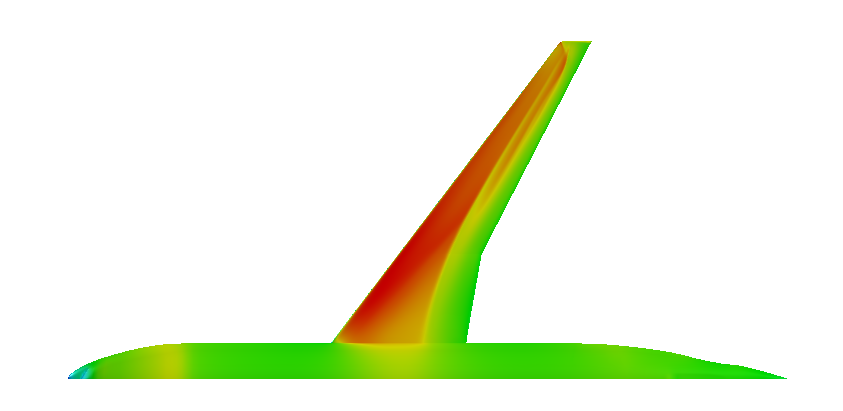
\includegraphics[width=0.45\textwidth]{images/part2/surfM85A2}\label{subfig:crmSnapshot}}
  \caption{CRM shape for aerodynamic simulations}
\end{figure*}

Again we use the elsA\textsuperscript{\textregistered} solver to perform simulations on the design. We use the $\kappa - \omega$ SST turbulence model to perform predictions since it has good performance in the fuselage wing interaction regions \cite{menter2003ten, vassberg2014summary}. The CFD was run for a combination of 21 values of $\alpha \in [1: 0.1: 3]$ and 5 values of $Mach \in [0.84: 0.005: 0.86]$, hence $N_{experiment} = 21\times5 = 105$. Figure, \ref{subfig:crmSnapshot} shows one of the pressure snapshots for $\alpha = 2$ and $Mach = 0.85$. We then cut the wing at four distinct locations $y/b = [0.105, 0.37, 0.5, 0.84]$ (figure \ref{subfig:crmWing}) to clearly observe different types of aerodynamic behavior. Here, $y$ denotes the y-distance from aircraft axis and $b$ denotes the span of one wing. 

As detailed in the earlier section we again use LOO-CV for comparing the performance of the two methods. The POD+I method has been run as described in appendix \ref{appPODI}. For GP regression, we learn a GP model between $y_{ij} = p_{ij}$ and input vector $\VEC{x_{ij}} = [x^{chord}_i, \alpha_j, Mach_j]$. We build a multi-dimensional kernel by multiplying 2 Mat\'ern kernels (for $\alpha$ and $Mach$ dimensions) and one Neural Network kernel (for $x^{chord}$ dimension). The shock will appear in the spatial dimension and hence using a Neural Network kernel in that dimension lets us capture the discontinuity more accurately. 

\begin{figure*}[!ht]
  \centering
  \subfigure[{Normalized RMSE for the two different model types. POD has a RMSE of $0.32\pm0.23$ whereas Distributed GPs has a RMSE of $0.02\pm0.01$. The average Distributed GPs prediction is 16 times better than POD in transonic regime. The outliers in the box-plots denote cases where the removed pairs are on the edges of database. Since the removed pairs are on the edges of database matrix, there are no CFD snapshots surrounding these pairs. Hence extrapolation is performed during the edge cases.}]
  {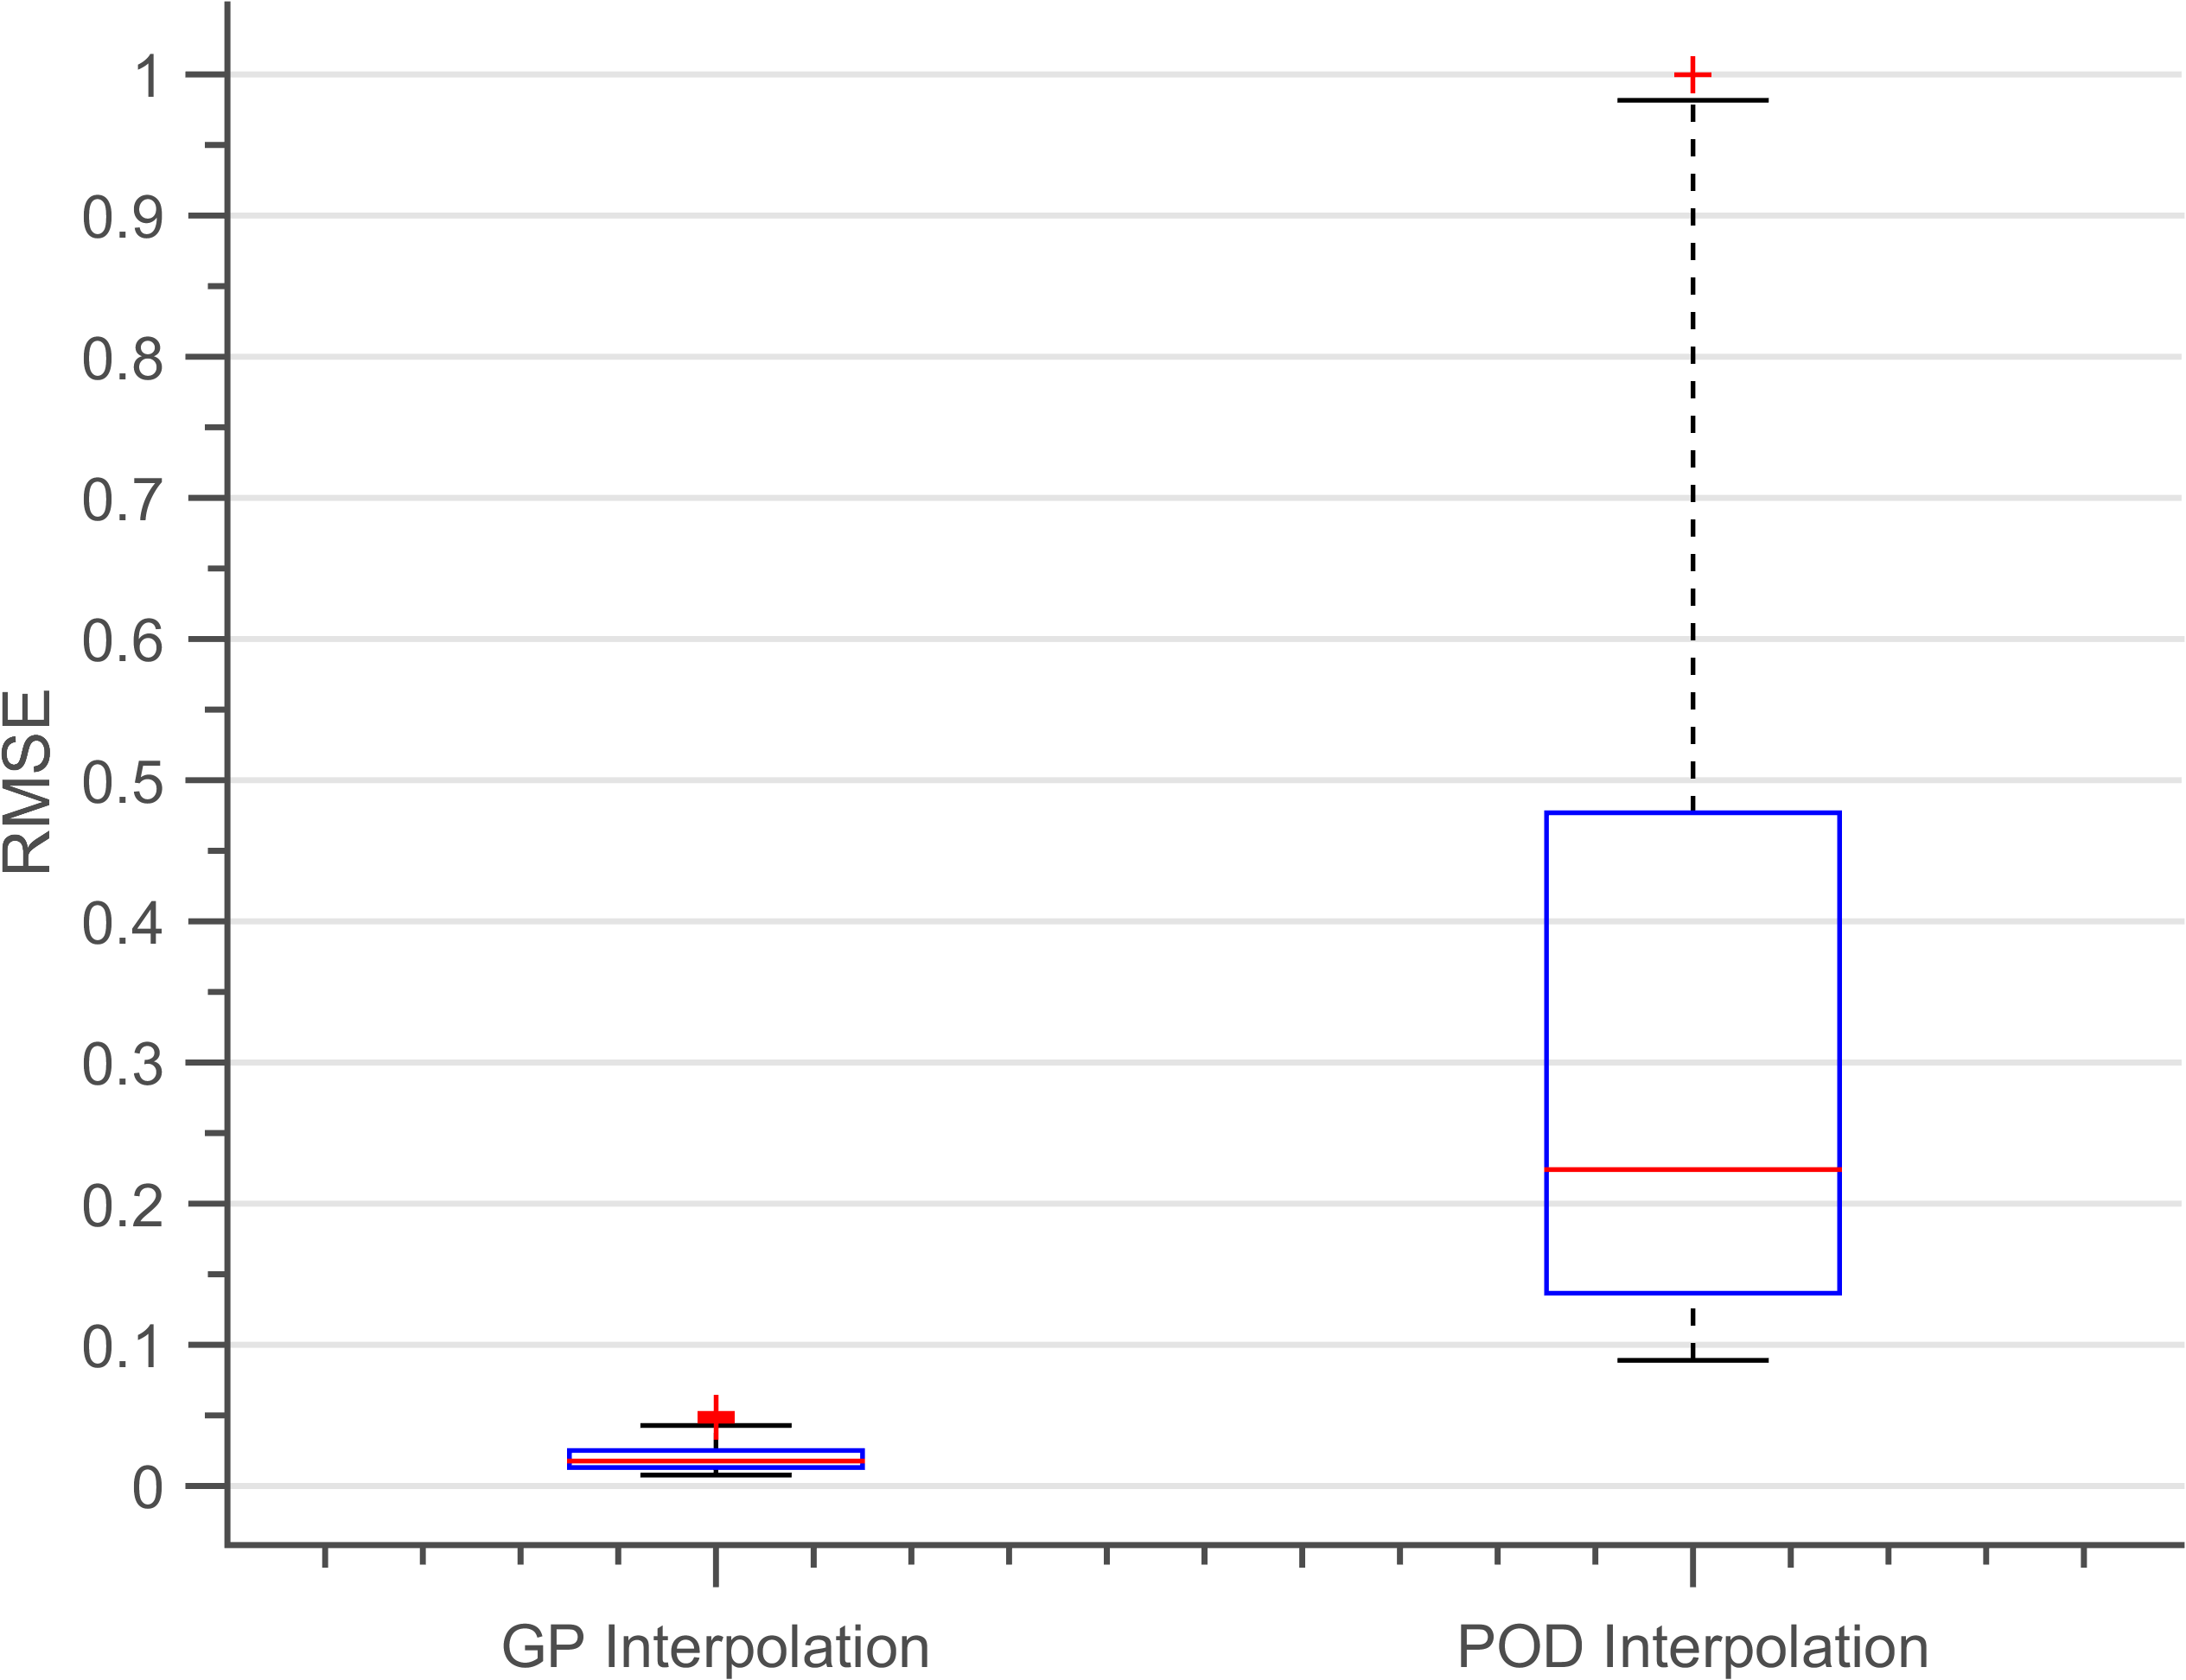
\includegraphics[width=0.45\textwidth]{images/part2/rmseCRM_box}\label{subfig:RMSECRM}}\quad
    \subfigure[{Time taken to perform prediction for the two different model types. POD takes $0.5s\pm0.03s$ whereas Distributed GPs takes $40.6s\pm2.3s$ to perform the interpolation. This is the time to perform prediction and not learning the model. The average POD method is 80 times faster than Distributed GPs.}]
    {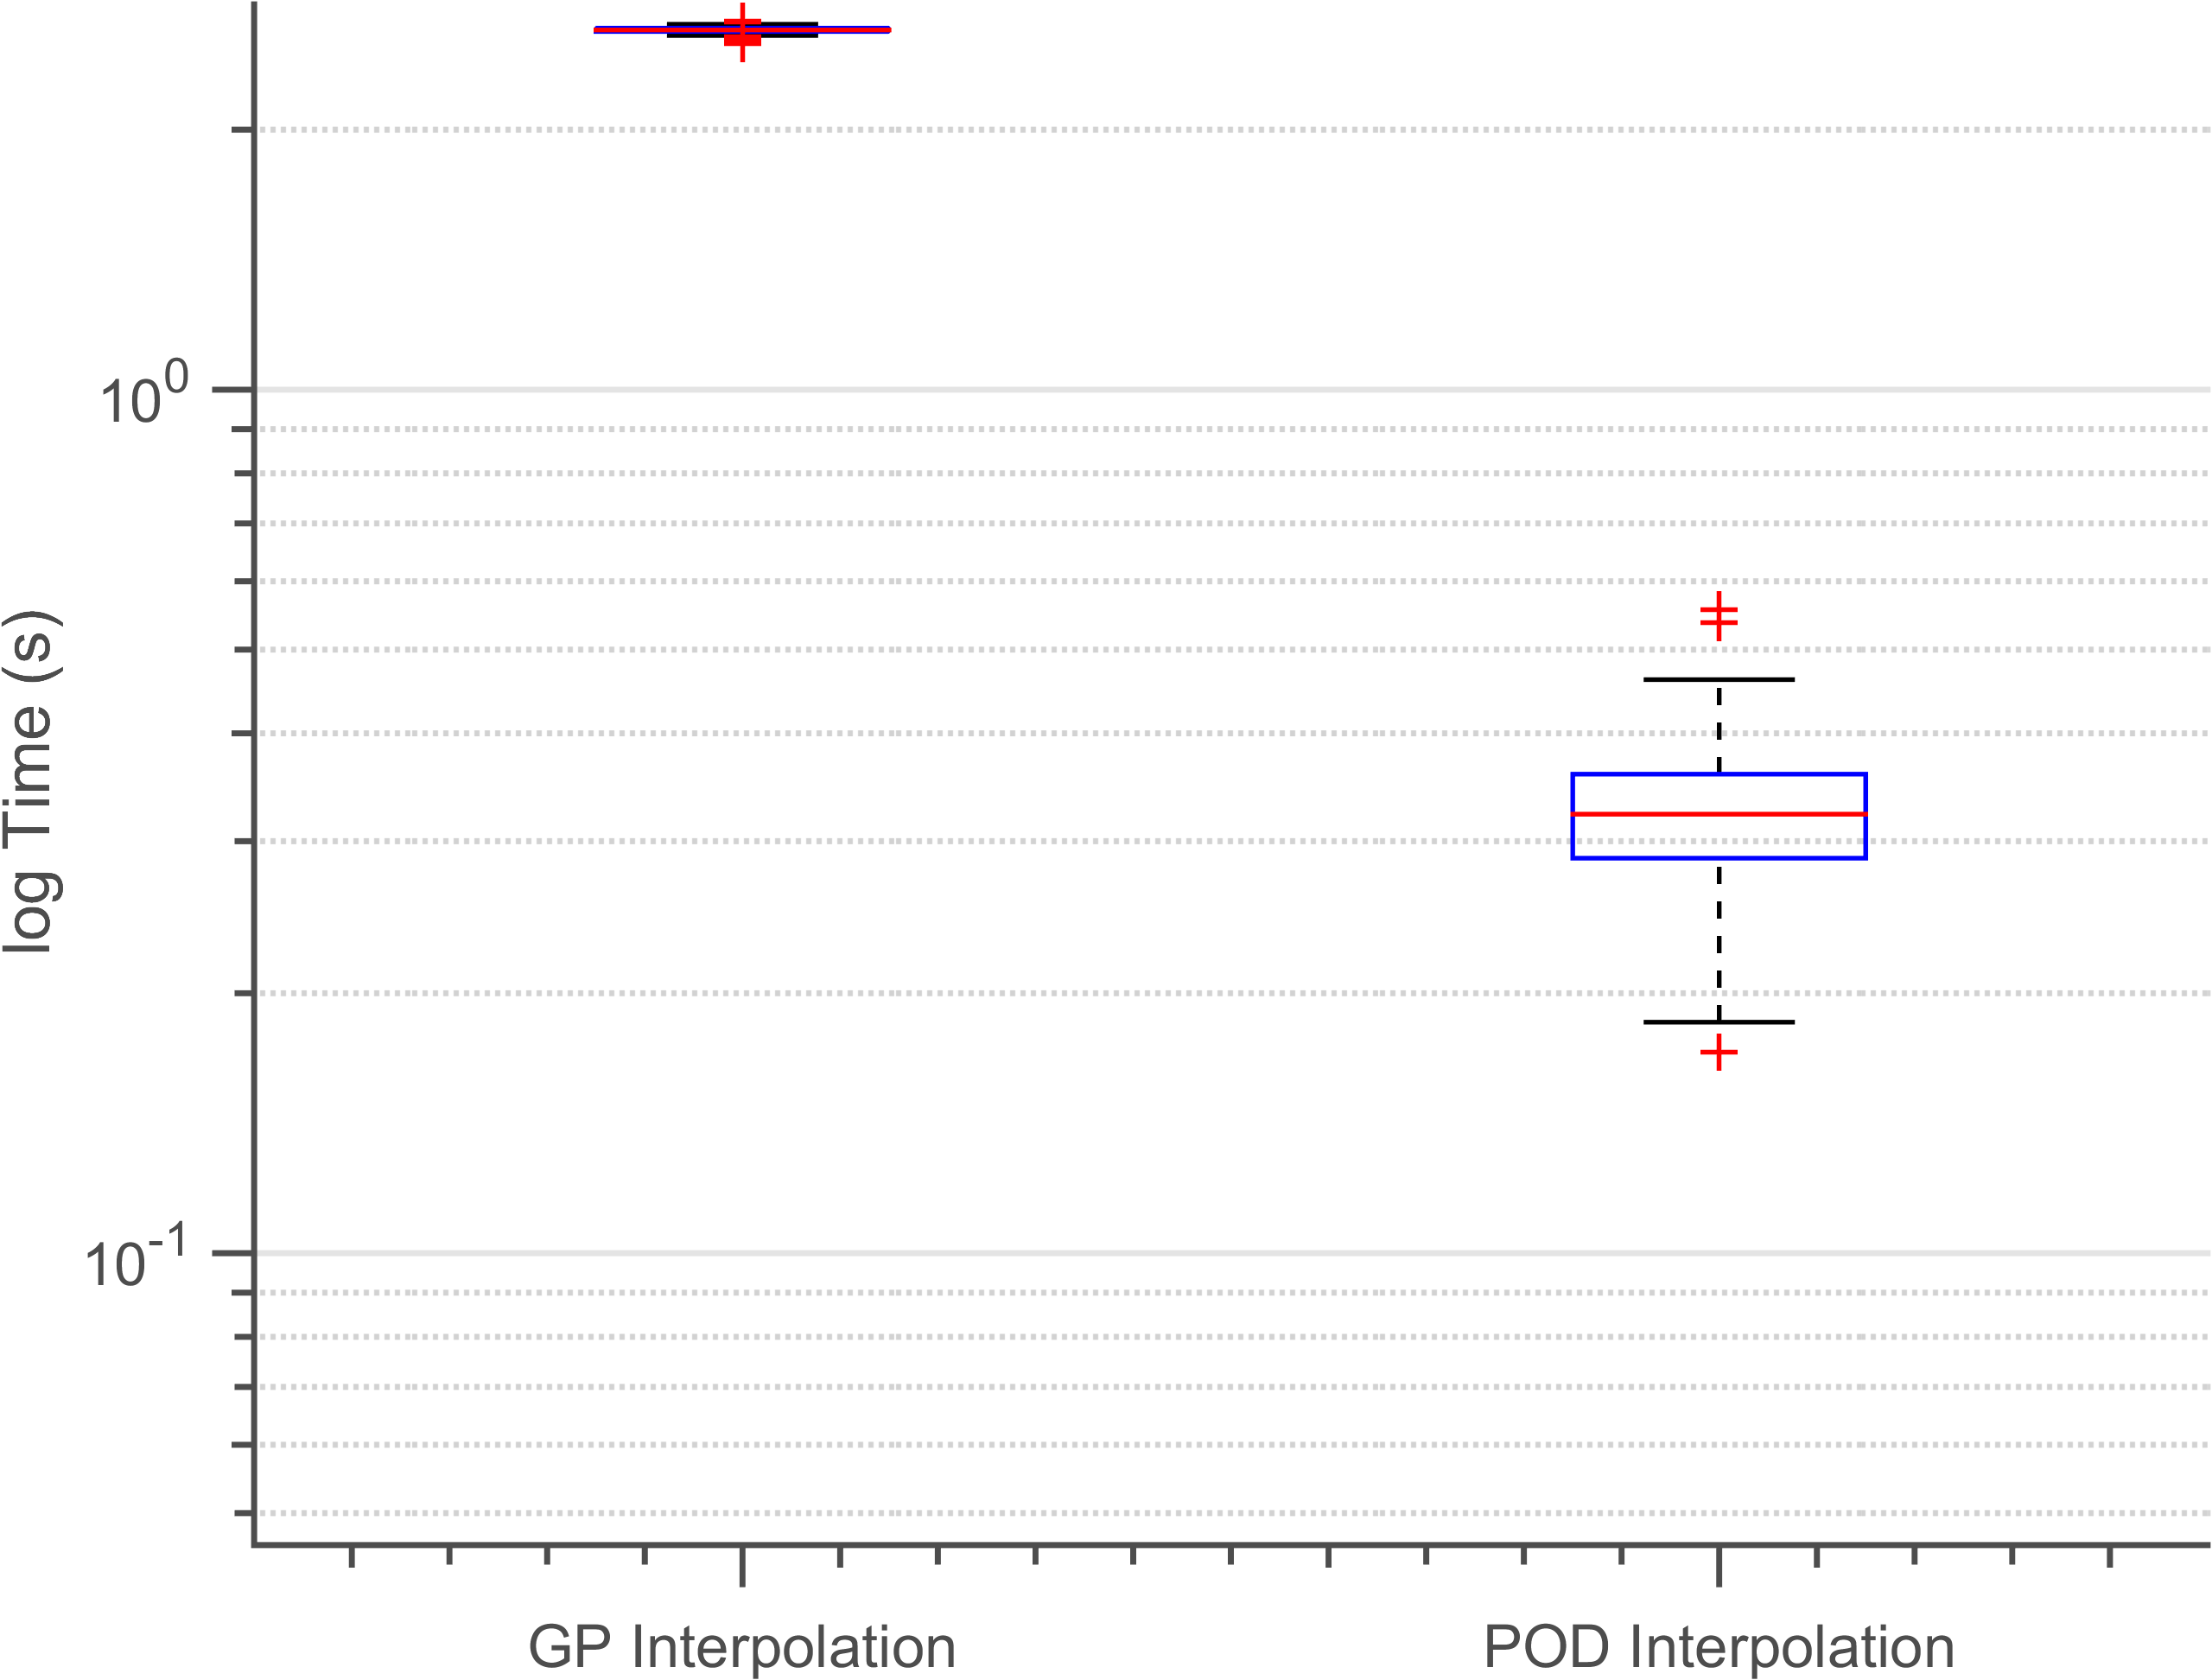
\includegraphics[width=0.45\textwidth]{images/part2/timeCRM_box}\label{subfig:timeCRM}}
  \caption{Results for CRM interpolation}
  \label{fig:resultsOnCRM}
\end{figure*}

\marginnote{\textsl{Figure \ref{fig:resultsOnCRM}}}[1cm]
Figure \ref{subfig:RMSECRM} denote the RMSE estimates for different pairs. POD has a RMSE of $0.32\pm0.23$ whereas Distributed GPs has a RMSE of $0.02\pm0.01$. The average Distributed GPs prediction is 16 times better than POD in transonic regime. The outliers in the box-plots denote cases where the removed pairs are on the edges of the domain. Since the removed pairs are on the edges of the domain, there are no CFD snapshots surrounding these pairs. Hence we are extrapolating on the outliers. Figure \ref{subfig:timeCRM} shows the time taken to perform prediction for the three different model types. POD takes $0.5s\pm0.03s$ whereas Distributed GPs takes $40.6s\pm2.3s$ to perform the interpolation. In transonic regime GP has a significantly better error performance and becomes the obvious choice for interpolation.

\begin{figure*}[!ht]
  \centering
  \subfigure[{Comparison between POD method and Distributed GPs for \textbf{interpolation}. The X-axis denotes chord dimension, only showing chord-section near shock for clarity. The Y-axis denotes the coefficient of pressure. Reconstruction is performed on the pressure snapshot at $\alpha = 2$ and $Mach = 0.85$ for the $y/b = 0.105$}. We can observe that the intensity of shock has been smoothed out by POD method]
  {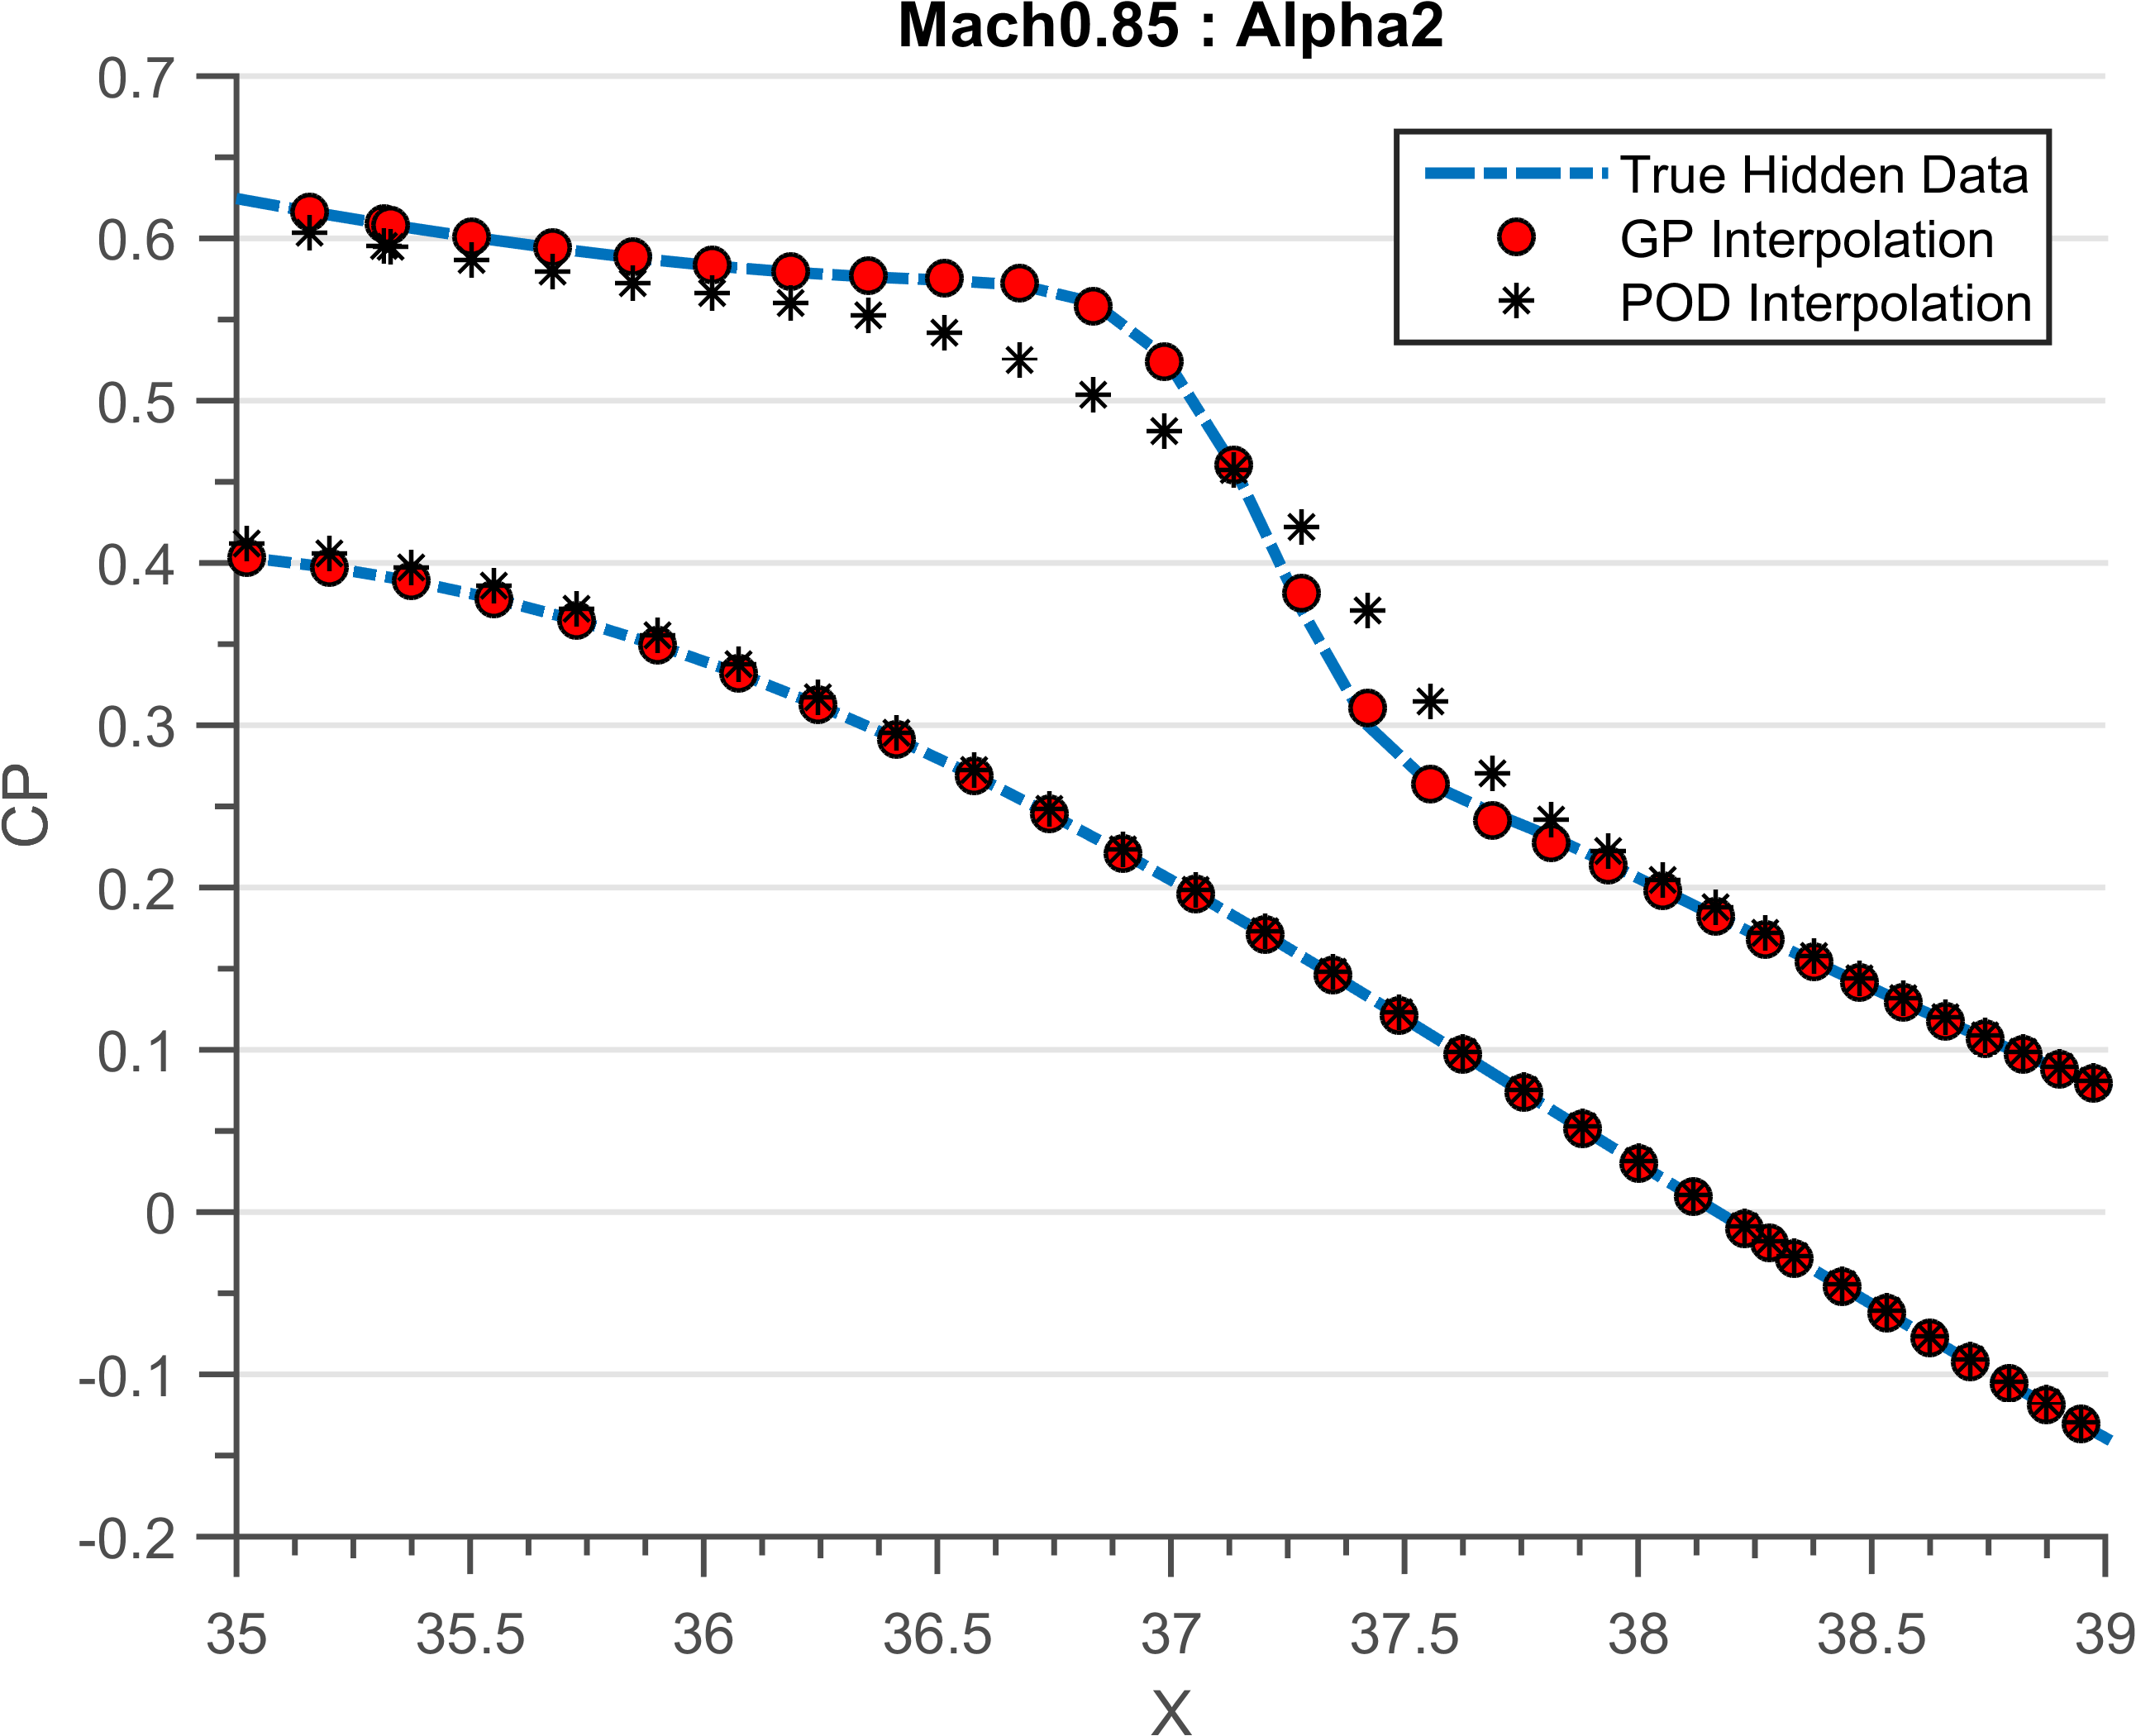
\includegraphics[width=0.45\textwidth]{images/part2/CRM-clean-testSnapshots_M850A20}\label{subfig:interpComparisonCRM}}\quad
    \subfigure[{Comparison between POD method and Distributed GPs for \textbf{extrapolation} (the extrapolation is being performed for the aerodynamic parameter ($Mach$) and not the spatial parameter). The X-axis denotes chord dimension, only showing chord-section near shock for clarity. The Y-axis denotes the coefficient of pressure. Reconstruction is performed on the pressure snapshot at $\alpha = 2$ and $Mach = 0.84$ for the $y/b = 0.105$. We can observe that POD introduces errors both for the intensity of shock and location of shock for this case}]
    {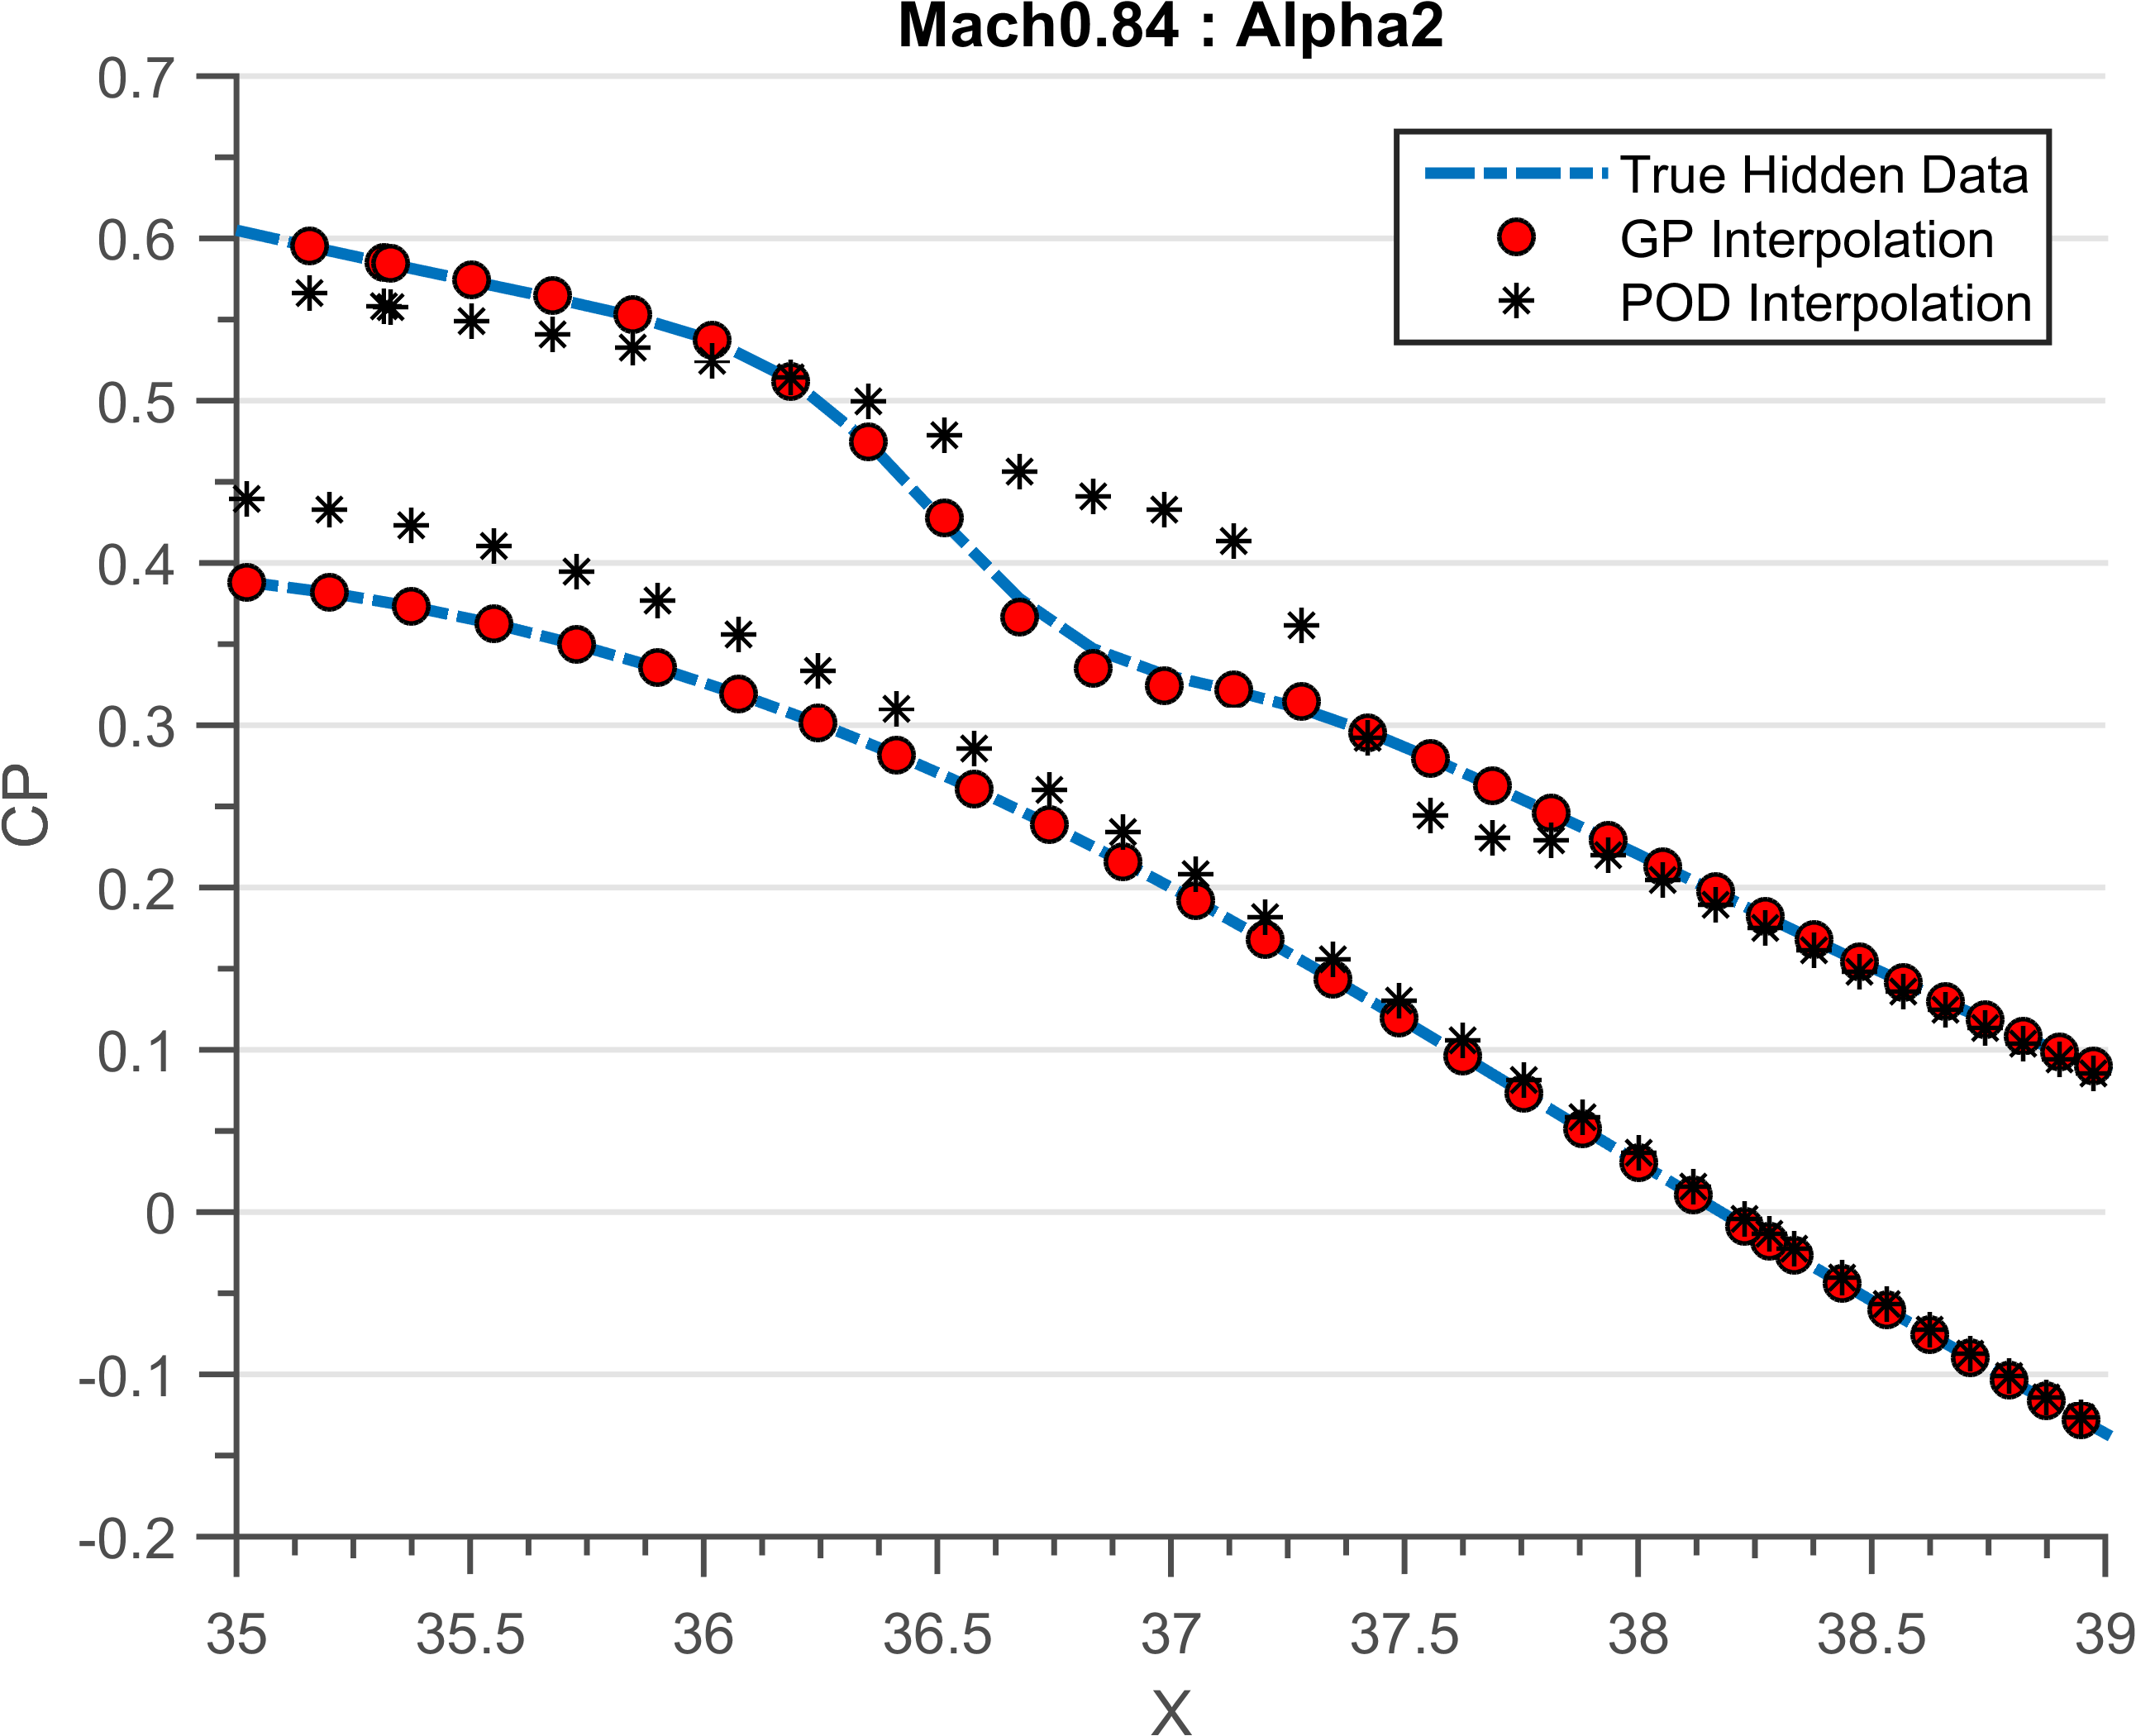
\includegraphics[width=0.45\textwidth]{images/part2/CRM-clean-testSnapshots_M840A20}\label{subfig:exterpComparisonCRM}}
  \caption{Comparison of pressure interpolations for first cut $y/b = 0.105$. Here we compare the accuracy of prediction for interpolation and extrapolation cases.}
  \label{fig:pressurePredictionsOnCRM}
\end{figure*}

\marginnote{\textsl{Figure \ref{fig:pressurePredictionsOnCRM}}}[1cm]
Figure \ref{subfig:interpComparisonCRM} shows the comparison between predicted pressures using the POD method and the Distributed GPs for case of interpolation. Reconstruction is performed on the pressure snapshot at $\alpha = 2$ and $Mach = 0.85$ for the $y/b = 0.105$. We can observe that the shape of shock has been smoothed out by the POD method. Figure \ref{subfig:exterpComparisonCRM} shows comparison between POD method and Distributed GPs for extrapolation, the extrapolation is being performed for the aerodynamic parameter ($Mach$) and not the spatial parameter. Reconstruction is performed on the hidden pressure snapshot of $\alpha = 2$ and $Mach = 0.84$ which is an extrapolation case. We can observe that POD introduces errors both for the intensity of shock, and location of shock for the extrapolation case, this explains the high amount of error in figure \ref{subfig:RMSECRM}.  

\subsubsection{Comparison across cuts}
We next study the accuracy of Distributed GPs for different airfoils on the wing. Using the methodology described earlier we build a Distributed GPs model for each airfoil and measure the accuracy of interpolation performed for each cut using the LOO-CV methodology. 

\begin{figure*}[!ht]
  \centering
  \subfigure[{Normalized RMSE for different airfoils based on Distributed GPs. The mean RMSE of different cuts from $y/b = [0.105, 0.37, 0.5, 0.84]$ is $[0.053, 0.17, 0.31, 0.40]$ respectively. The accuracy of interpolation deteriorates as we go farther away from the fuselage. This is due to appearance of double shock on the outer section of wing.}]
  {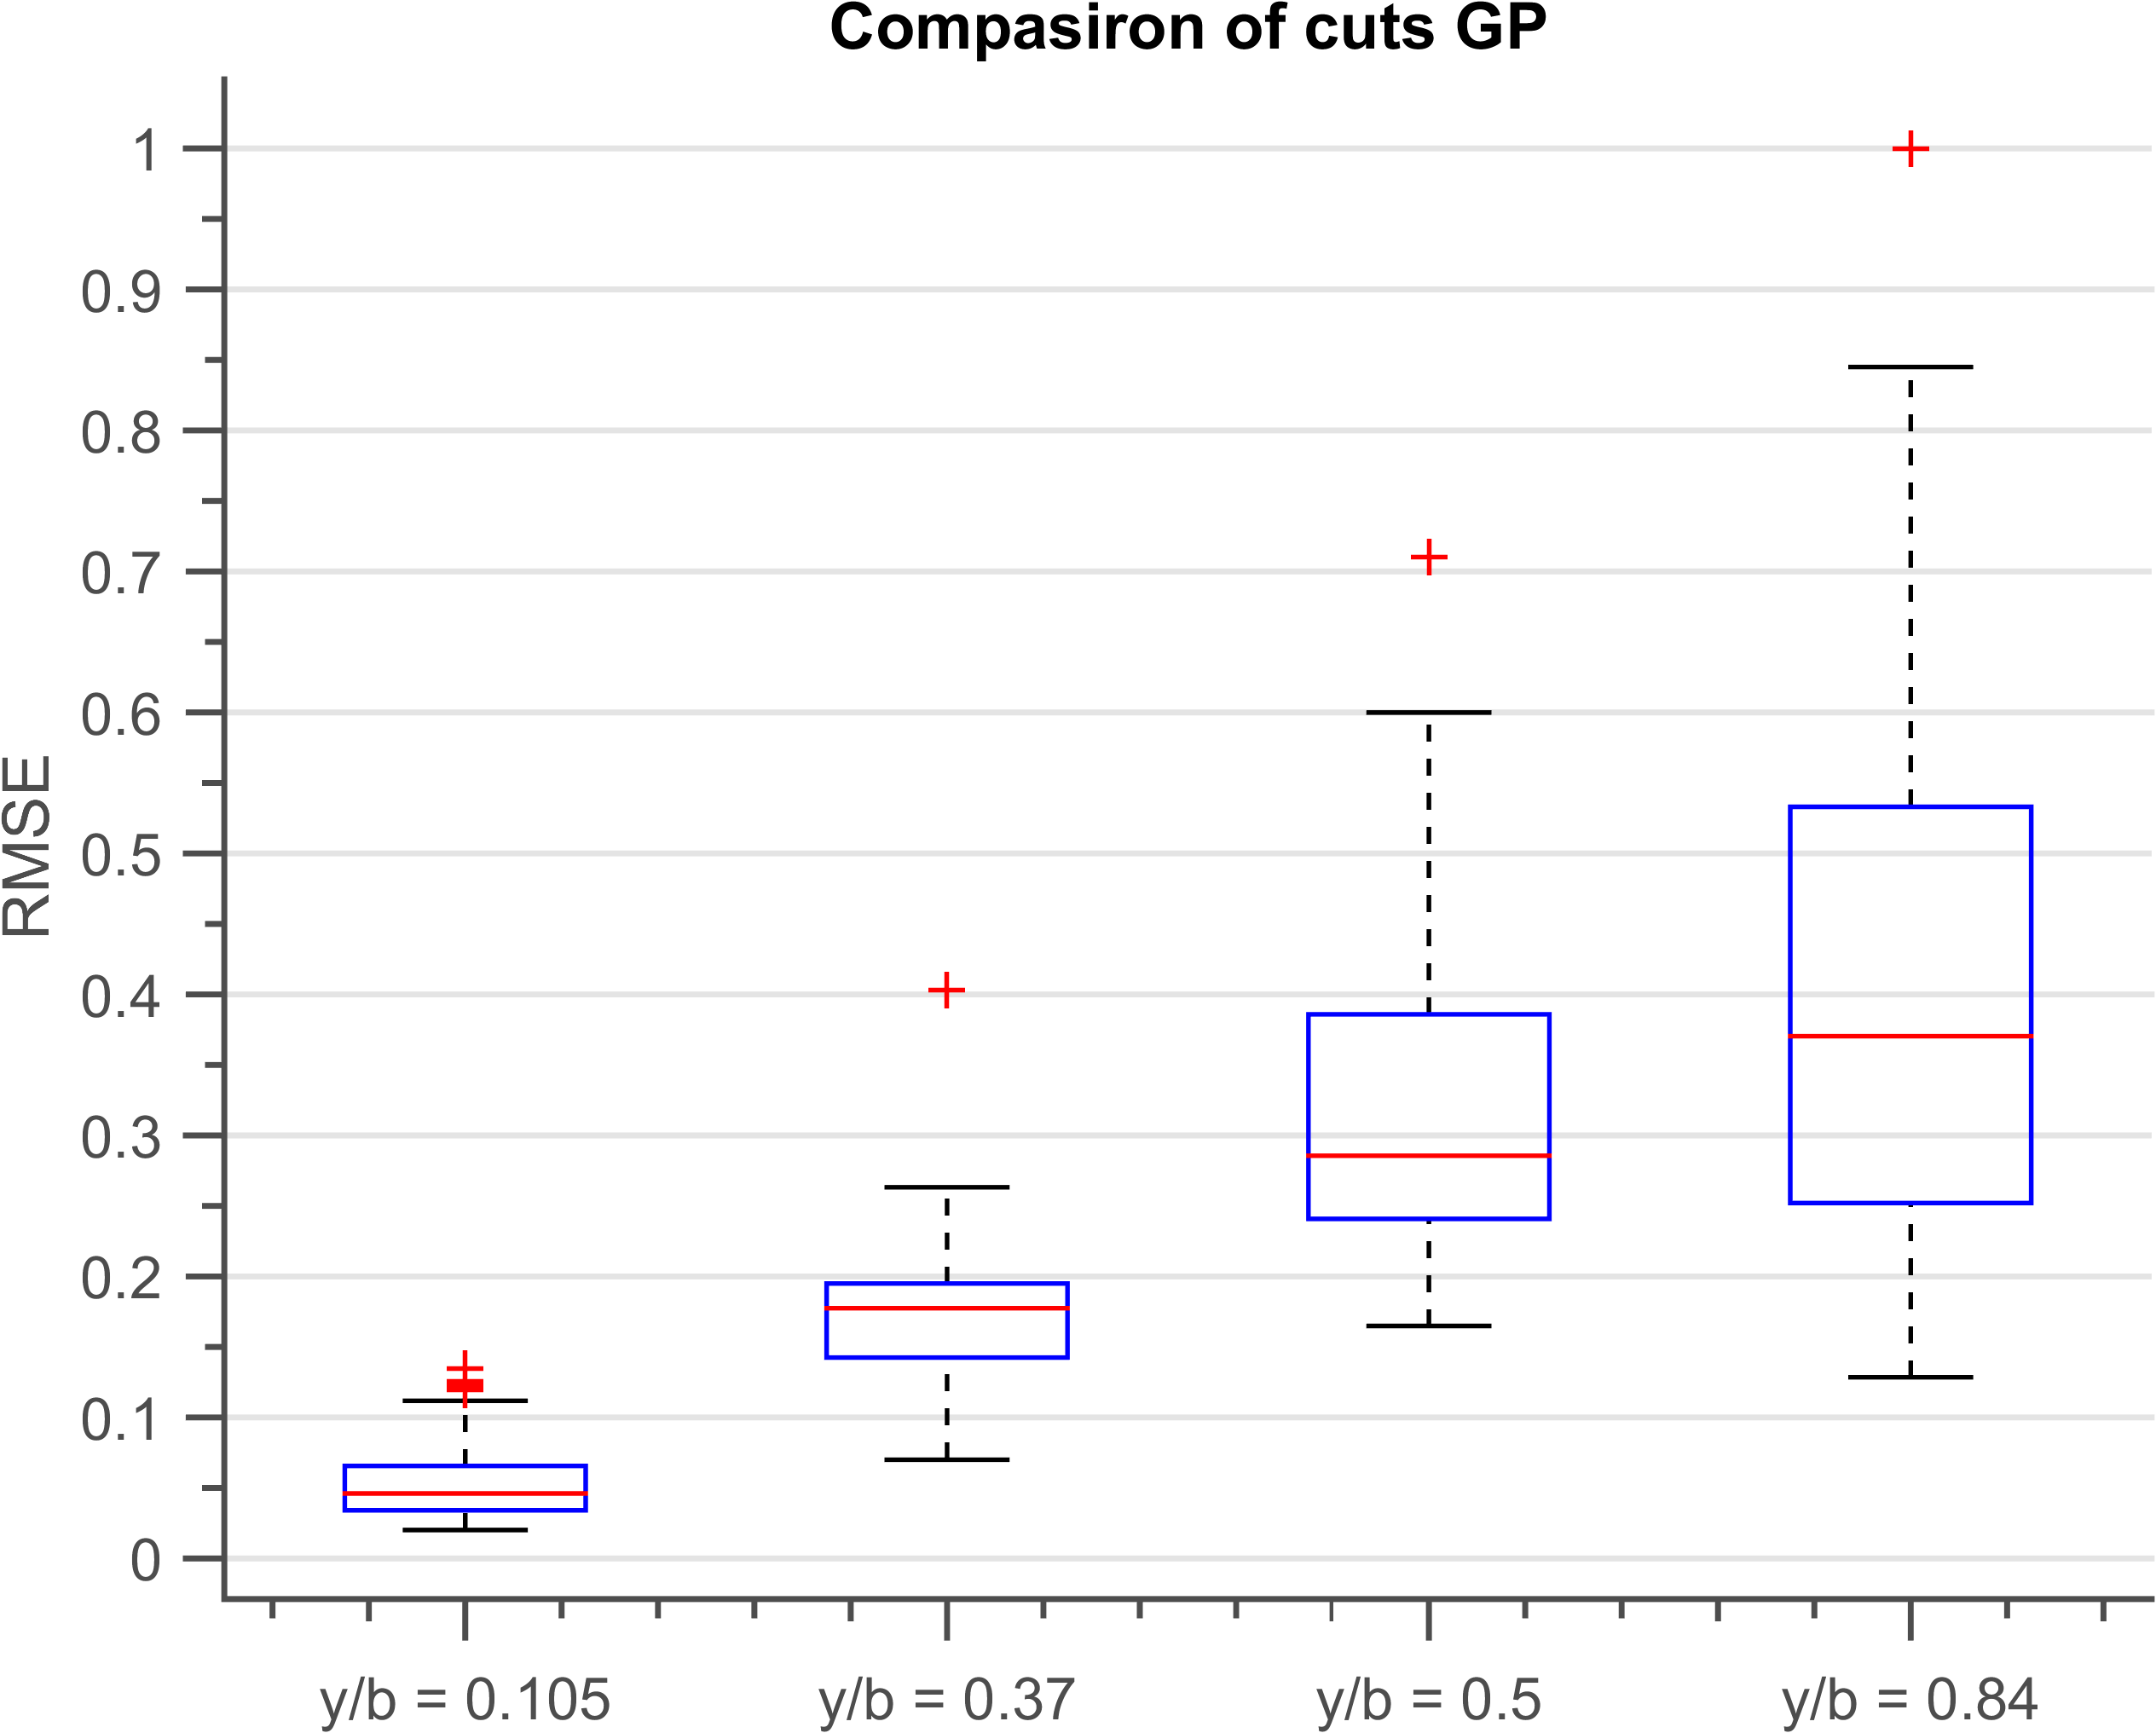
\includegraphics[width=0.45\textwidth]{images/part2/compasironOfCutsGPCRM_box}\label{subfig:compasironOfCutsGPCRM}}\quad
    \subfigure[{Comparison between POD method and Distributed GPs for interpolation. The X-axis denotes chord dimension, only showing chord-section near shock for clarity. The Y-axis denotes the coefficient of pressure. Reconstruction is performed on the pressure snapshot at $\alpha = 2$ and $Mach = 0.85$ for the location  $y/b = 0.84$}. While POD smooths out the double shock pattern Distributed GPs also lacks the accuracy observed in figure \ref{subfig:interpComparisonCRM}.]
    {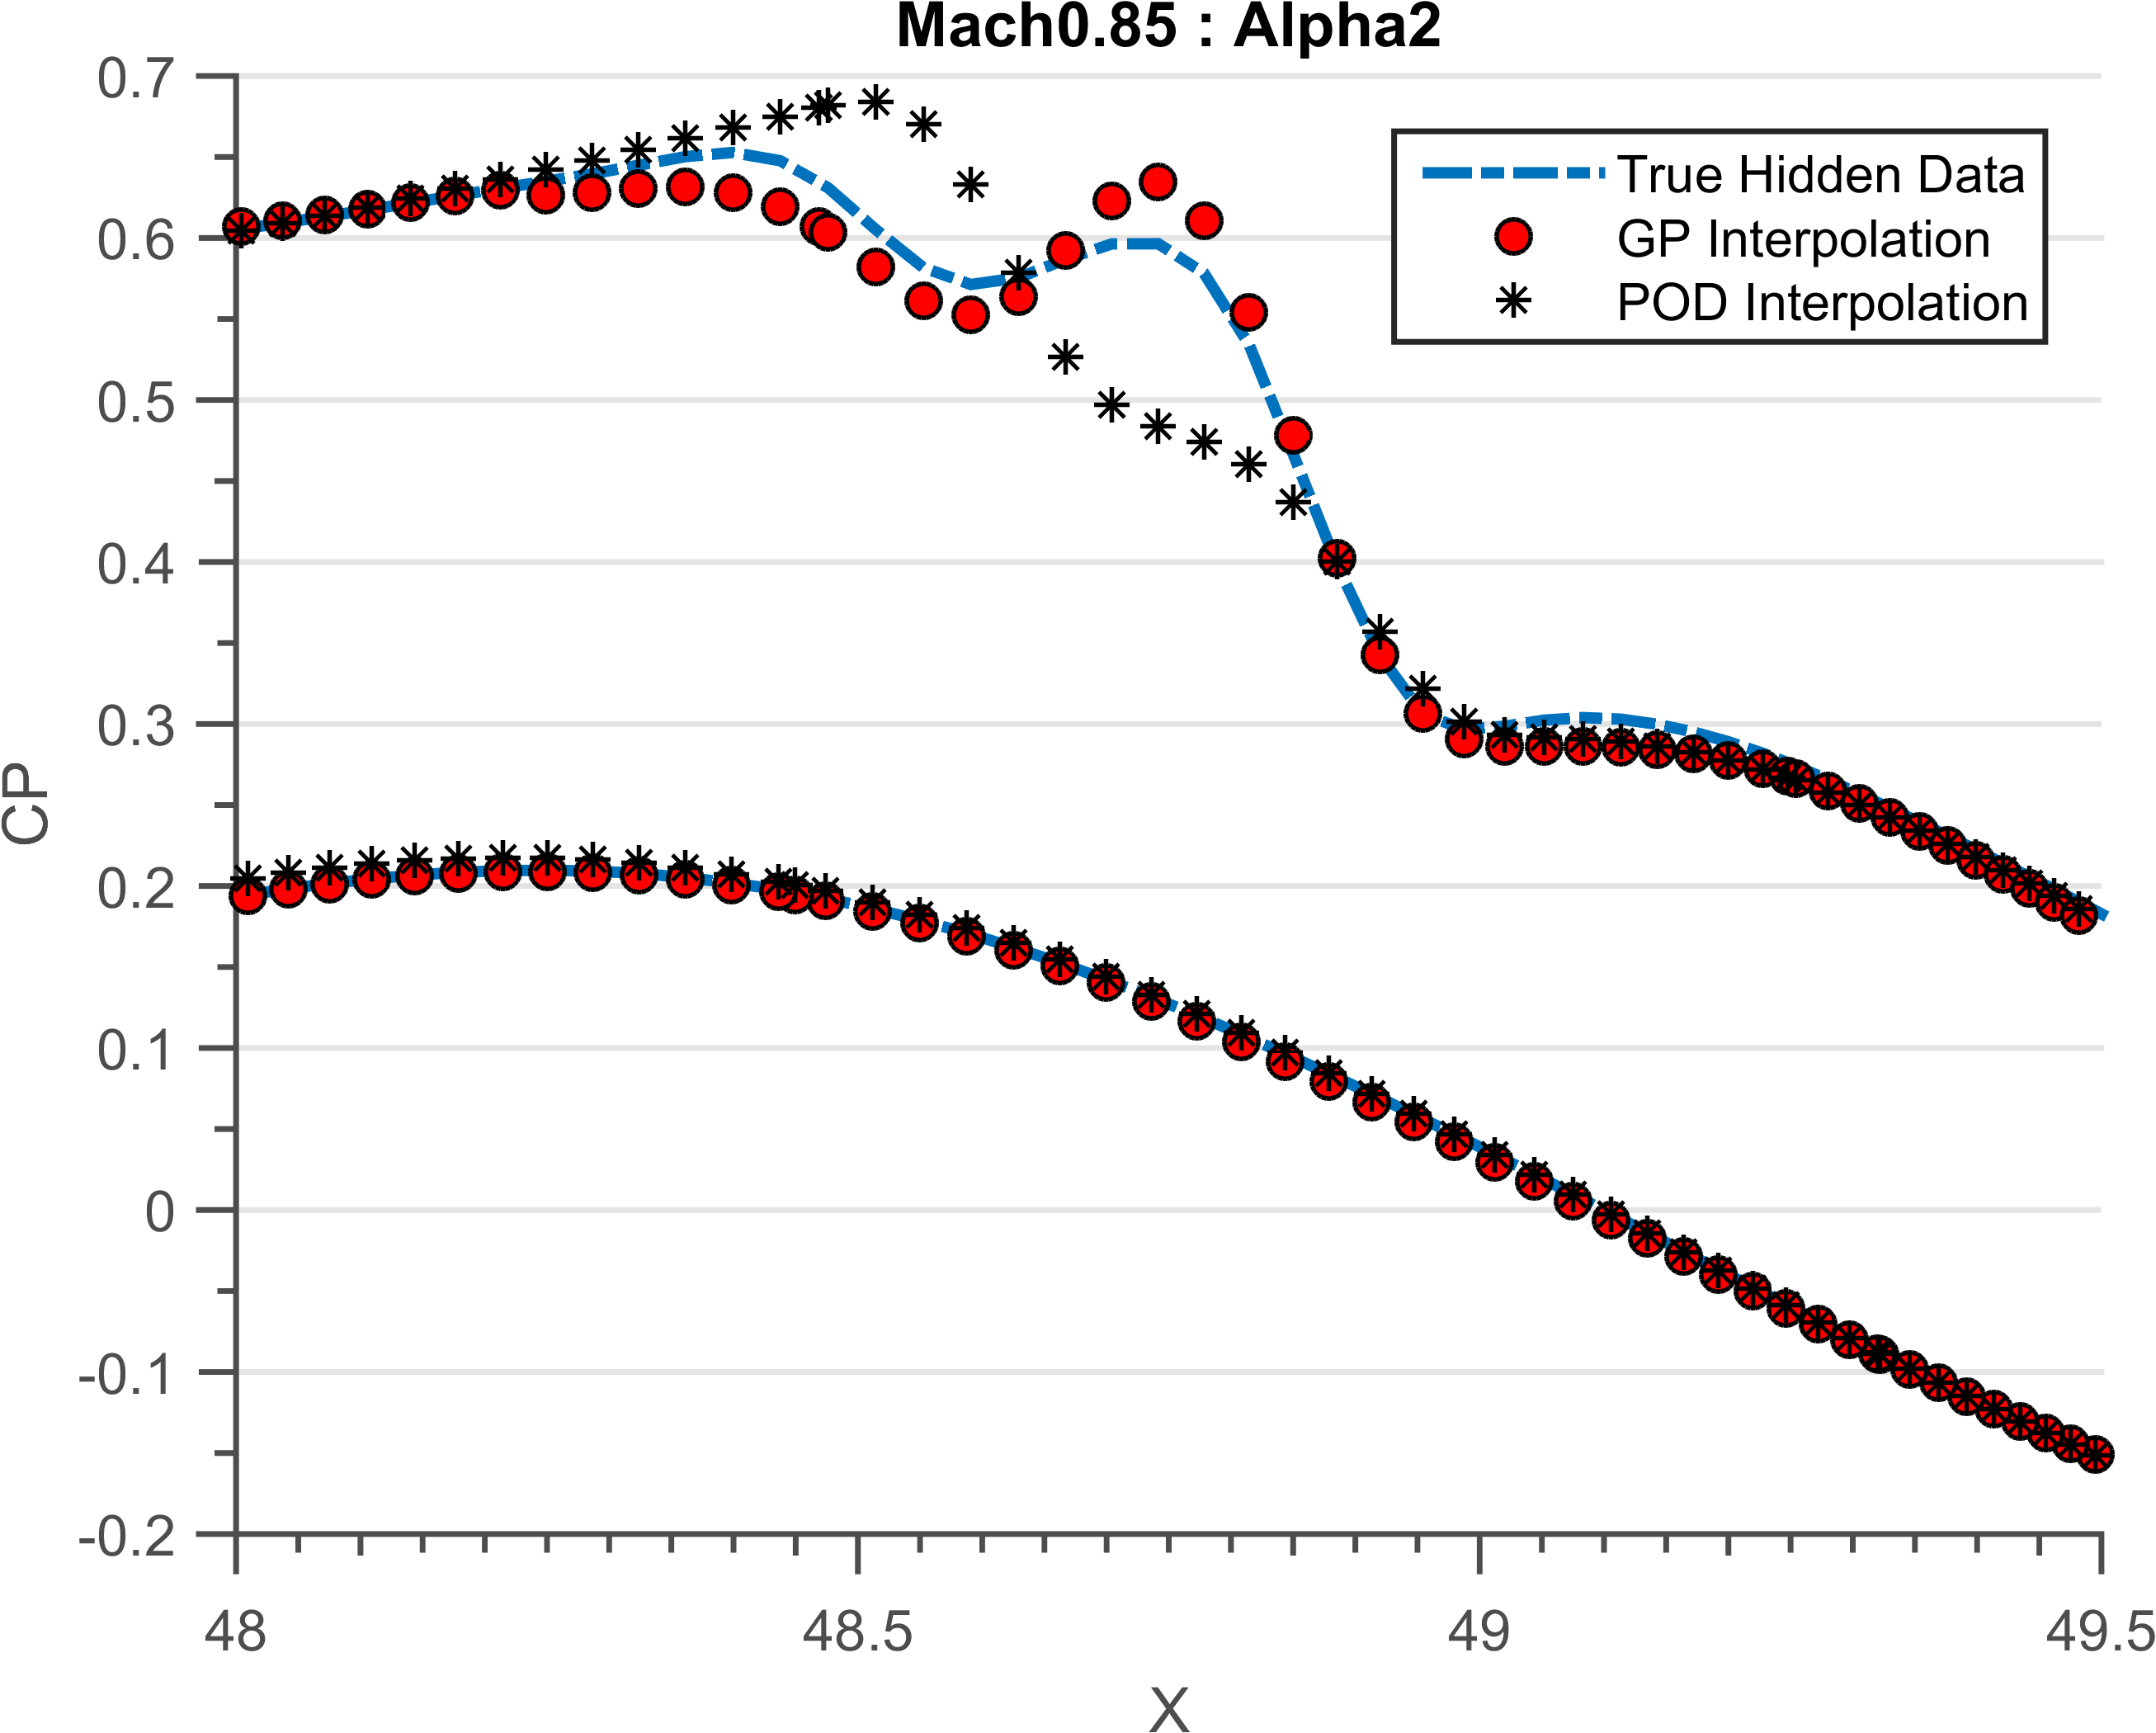
\includegraphics[width=0.45\textwidth]{images/part2/CRM-clean-testSnapshots_M850A20_cut4}\label{subfig:interpCut4}}
  \caption{Performance of Distributed GPs across cuts}
  \label{fig:CRMPerformanceAcrossCuts}
\end{figure*}

\marginnote{\textsl{Figure \ref{fig:CRMPerformanceAcrossCuts}}}[1cm]
Figure \ref{subfig:compasironOfCutsGPCRM} shows the RMSE performance across cuts. The performance of interpolation deteriorates as we go further away from the fuselage. This is primarily because as we go further away from the fuselage double shocks start appearing on the airfoil as observable from figure \ref{subfig:crmSnapshot}. Figure \ref{subfig:interpCut4} shows interpolation performed by the POD method and Distributed GPs methods at $\alpha = 2$ and $Mach = 0.85$, for the last cut ($y/b = 0.84$). While, POD smooths out the double shock pattern, Distributed GPs lacks the accuracy observed in figure \ref{subfig:interpComparisonCRM}. 

\begin{figure*}[!ht]
  \centering
  \subfigure[{Interpolation performed at constant $Mach = 0.845$ and $\alpha = [1, 3]$ for the location $y/b = 0.105$. The color coding denotes coefficient of pressure for upper side of airfoil, The x-axis denotes chord-wise location and y-axis denotes $\alpha$. White lines denote presence of a pressure snapshot due to CFD run, everything in between is interpolation. Dashed black lines denote constant pressure contours color between two contours has been smoothed for clarity. We observe a strong shock near $\alpha = 3$ which slowly gets converted to a weak shock near $\alpha = 1$.}]
  {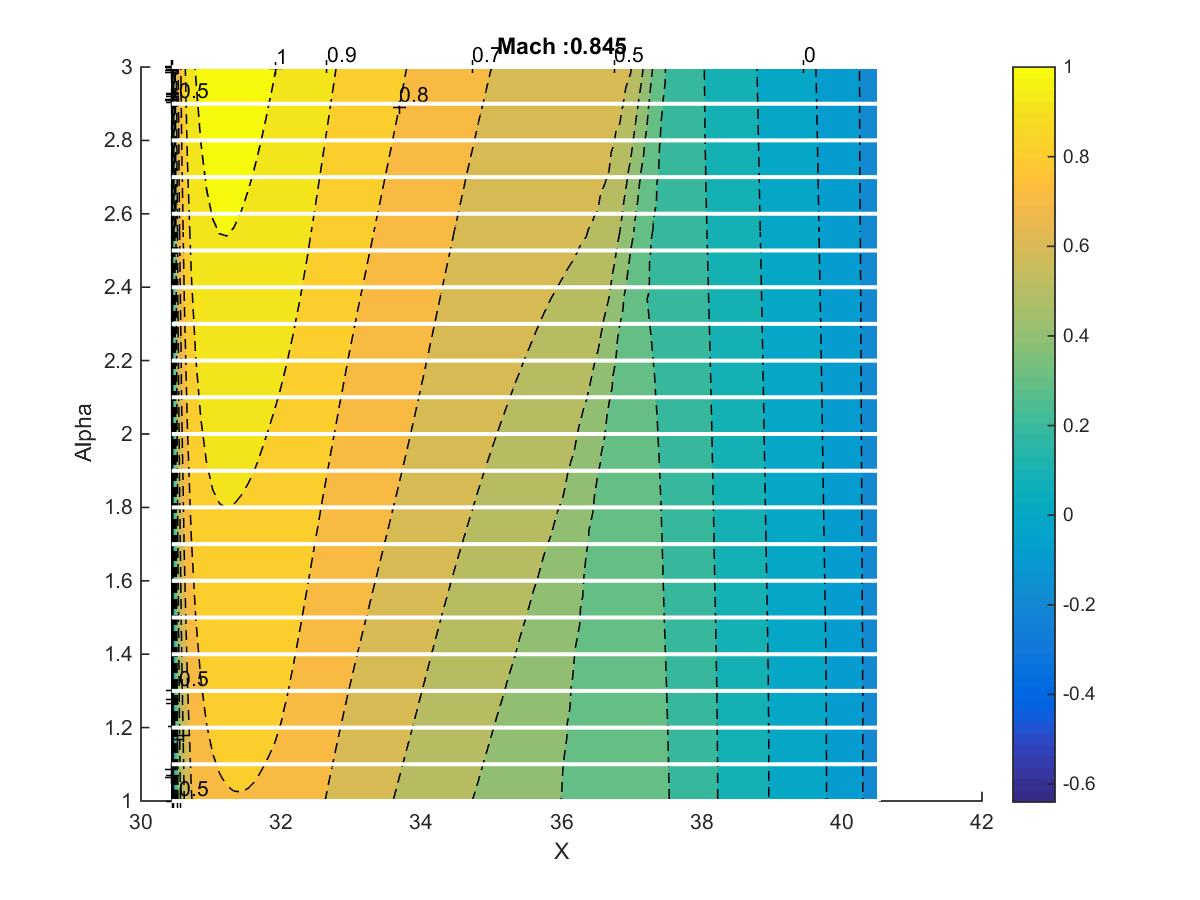
\includegraphics[width=0.45\textwidth]{images/part2/CRM-clean-testSnapshots_cut1_MachSweepContF845}\label{subfig:alphaSweepCut1}}\quad
    \subfigure[{Interpolation performed at constant $Mach = 0.845$ and $\alpha = [1, 3]$ for the location $y/b = 0.84$. The color coding denotes coefficient of pressure for upper half of airfoil, The x-axis denotes chord-wise location and y-axis denotes $\alpha$. White lines denote presence of a pressure snapshot due to CFD run, everything in between is interpolation. Dashed black lines denote constant pressure contours color between two contours has been smoothed for clarity. We observe a single shock near $\alpha = 3$ which slowly gets converted to a double shock pattern.}]
    {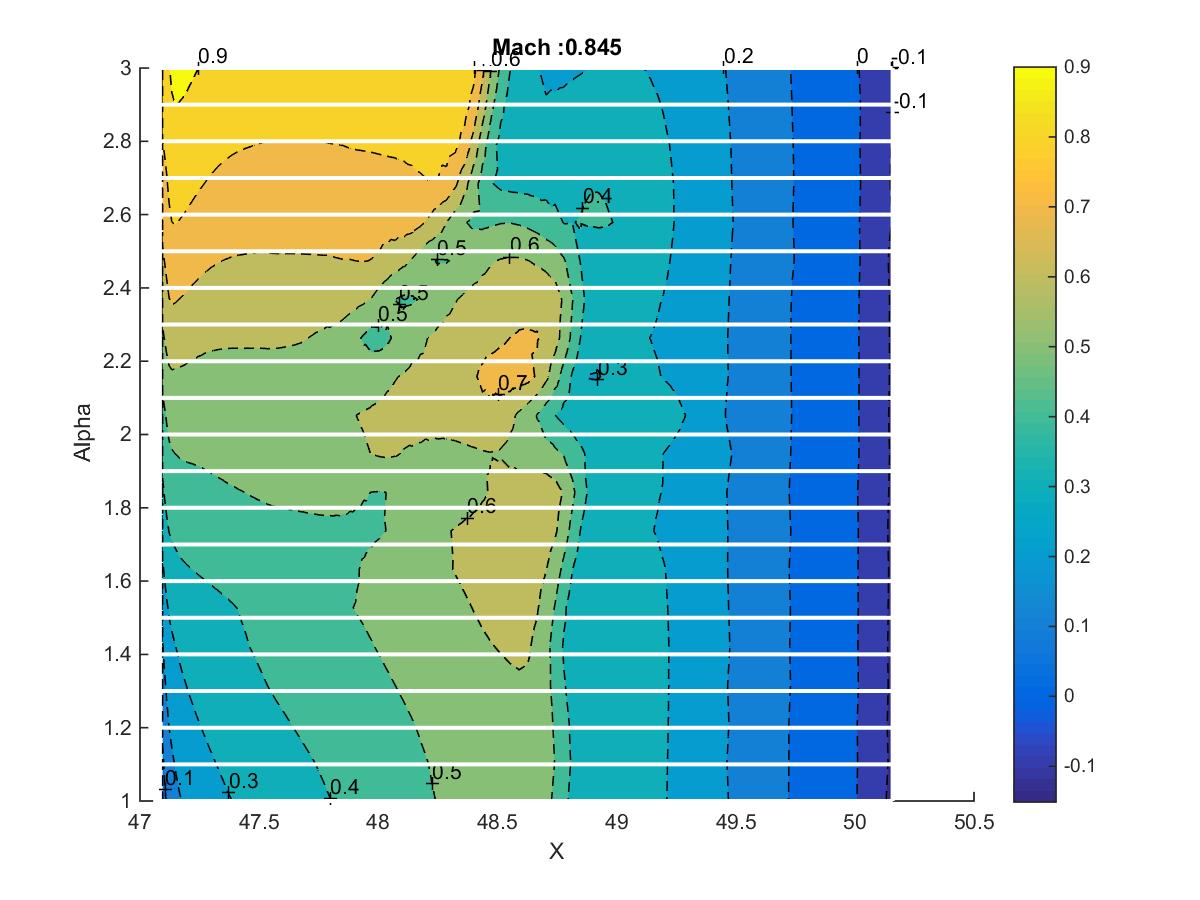
\includegraphics[width=0.45\textwidth]{images/part2/CRM-clean-testSnapshots_cut4_MachSweepContF845}\label{subfig:alphaSweepCut4}}
  \caption{Pressure reconstructions for constant $Mach = 0.845$ and sweeping $\alpha \in [1, 3]$}
  \label{fig:pressureReconstructionCRM}
\end{figure*}

Figures \ref{subfig:alphaSweepCut1} and \ref{subfig:alphaSweepCut4} show the evaluation of pressures upon varying $\alpha \in [1, 3]$ at locations $y/b = 0.105$ and $y/b = 0.84$ respectively. The color coding denotes coefficient of pressure for the upper side of airfoil, The x-axis denotes chord-wise location and y-axis denotes $\alpha$. White lines denote presence of a pressure snapshot due to CFD run, everything in between is interpolation. Dashed black lines denote constant pressure contours Color between two contours has been smoothed for clarity. For figure \ref{subfig:alphaSweepCut1} we observe a strong shock near $\alpha = 3$ which slowly gets converted to a weak shock near $\alpha = 1$. The presence of a single shock is also the reason why Distributed GPs performs better at this cut location. For figure \ref{subfig:alphaSweepCut4} we observe a single shock near $\alpha = 3$ which slowly gets converted to a double shock pattern. The zone from single to double shock is a very interesting point for performance, since the wing drag is minimum during this transition phase. Distributed GPs starts performing badly near the transition phases, this can be observed by the small pools of $C_{P} = 0.5$ at the transition phase from single to double shock. 
\marginnote{\textsl{Double shocks}}[-3cm]

The current section presents a comparison between two different surrogate model building methods: time-tested surrogate modelling methods such as POD coupled with spline interpolation and upcoming machine learning methods such as Distributed GPs for subsonic and transonic regimes. The Distributed GPs performs marginally better than POD technique in subsonic regime but is many times slower. On the contrary for the case of transonic regime Distributed GPs clearly outperforms POD+I method. This is mainly due to the presence of shock on the airfoil. 

Plots like figure \ref{subfig:alphaSweepCut4} give a quick understanding of the flight regime for very few simulation runs. These plots can also be used to find transition regimes from single shock to double shock, which are very interesting performance points. In the future we wish to improve reconstruction of double shock patterns by improving the length scale and improve the choice of experts for Distributed GPs.

\section{Summary and discussion}\label{subsec:ExpressingStructureKernelConclusion}
In the last two chapters we have tried to answer the question: How to add \textit{a-priori} information of a pattern in a learning algorithm? We present a sample of the wide variety of available covariance functions. Due to the ability to create new kernels, encoding prior information into the structure can be performed easily. If we have an \textit{a-priori} information about the pattern of function to be learned, then embedding this information into the GP algorithm greatly improves accuracy and cost of prediction. Table \ref{tabListOfCombinationOfCovarianceFunctions} lists a few commonly known combinations of covariance functions in the literature. 

%\renewcommand{\arraystretch}{1}
%\begin{comment}
\begin{table}[!ht]
    \centering
\begin{tabularx}{\textwidth}{|l|l|X|}
  \hline
Model  & Structure & Citation \\
  \hline 
  \hline
Linear Regression & \small $k_{constant}+k_{linear}+k_{noise}$ &  \normalsize\\
Polynomial & \small $k_{constant}+\prod k_{linear}+k_{noise}$ &  \normalsize\\
Ordinary kriging & \small $k_{SE} + k_{noise}$ \normalsize &  \cite{krige1951statistical} \\
Simple kriging & \small $k_{constant}+k_{SE} + k_{noise}$ &  \normalsize\\
Universal Kriging & \small $\prod k_{linear}+k_{SE} + k_{noise}$ \normalsize & \cite{matheron1963principles} \\ Multiple Kernel & \small $\sum k_{SE} + k_{noise}$ \normalsize  &  \\
Spectral Mixture & \small  $\sum cos k_{SE} + k_{noise} ]$ \normalsize & \cite{wilson2013gaussian} \\
Change point & \small  $\sum CP(k_{Lin}, k_{SE}) + k_{noise} ]$ \normalsize & \cite{osborne2010bayesian} \\
Additive GPs & \small  $\prod_{i}(1+k^{i}_{SE}) ]$ \normalsize& \cite{duvenaud2011additive} \normalsize\\
   \hline
\end{tabularx}
  \caption{Combination of covariance functions available in literature}
  \label{tabListOfCombinationOfCovarianceFunctions}
  \end{table}
%\end{comment}

Section \ref{secSingleDimension} describes how to combine kernels to create one-dimensional kernels. While section \ref{subsubsecCh4ApplicationCP} describes how to build kernels for higher dimensions. There are two main contributions of this chapter, first we develop a novel methodology to detect the start of a non-linear regime in an engineering design problem. This is thanks to the change-point kernel which lets us define change from one regime to another \cite{chiplunkar:hal-01555401}. Second, we encode the information of shock to interpolate pressures in the transonic regime. This strategy gives significant gains in accuracy when compared to the standard POD+I for aerodynamic interpolation \cite{oatao18004}. 

In the next two chapters we will tackle the remaining questions posed in section \ref{secCh1Contributions} of the thesis. Chapter \ref{chapMultiTaskExtrapolation} discusses how to perform extrapolation given a computer simulation of experiments, while chapter \ref{chapAddingEquationsInGP} discusses how to encode prior information of relationships between measurements into a GP regression. 
